\documentclass[a4paper,10pt]{article} % Artikel med 12pt text och A4 storlek.
%\documentclass[draft,10pt]{article} % Artikel med 12pt text och A4 storlek.
\usepackage[english]{babel} % Svensk avstavning istället för engelsk
%\usepackage[pdflatex]{graphicx}% De här två behövs för svenska
\usepackage[utf8]{inputenc} % UTF-8 encodad fil. Kan bytas ut mot latin1 om en vill...
\usepackage[T1]{fontenc}
\usepackage[authoryear]{natbib}
\usepackage{bibentry}
\usepackage{subcaption}
\usepackage{boldline} 
%\usepackage[allfiguresdraft]{draftfigure}
\usepackage{float}
\usepackage[margin=2.5cm]{geometry}
\usepackage{setspace}
\usepackage{color}
\usepackage{enumitem}   
\usepackage[T1]{tipa}
\usepackage{tabu}
\usepackage{textcomp}
\usepackage{rotating}
\usepackage{booktabs}
\renewcommand{\arraystretch}{1.3}
\usepackage{tabu}
\usepackage{longtable}
\usepackage{pbox}
\usepackage{setspace}
\usepackage{lscape}
%\usepackage{enumitem}
%\usepackage{enumerate}
\setcounter{secnumdepth}{4}
\setcounter{tocdepth}{5}
\usepackage{array}
\newcolumntype{?}{!{\vrule width 1pt}}
\newcolumntype{L}[1]{>{\raggedright\let\newline\\\arraybackslash\hspace{0pt}}m{#1}}
\newcolumntype{C}[1]{>{\centering\let\newline\\\arraybackslash\hspace{0pt}}m{#1}}
\newcolumntype{R}[1]{>{\raggedleft\let\newline\\\arraybackslash\hspace{0pt}}m{#1}}
%\usepackage{graphics}
\usepackage{graphicx}
\usepackage{subcaption}

\usepackage{lipsum}



\usepackage{footnote}
\usepackage{tipx}

\usepackage{wrapfig}
\usepackage[table,dvipsnames]{xcolor}
\usepackage{multirow}

\usepackage{titlesec}

\setcounter{secnumdepth}{4}


\usepackage{color}  
\usepackage{hyperref}
\hypersetup{
    colorlinks=true, %set true if you want colored links
    linktoc=all,     %set to all if you want both sections and subsections linked
    linkcolor=violet,  %choose some color if you want links to stand out
            urlcolor=blue,
            citecolor=Thistle,
}

\usepackage{xcolor}

\definecolor{hedvig_blue}{HTML}{7D81F5}
\definecolor{hedvig_lightgreen}{HTML}{81F093}
\definecolor{hedvig_darkgreen}{HTML}{0B8C1F}
\definecolor{hedvig_orange}{HTML}{FFB87A}
\definecolor{hedvig_red}{HTML}{FFD9E0}
\definecolor{hedvig_yellow}{HTML}{FCFFA8}



\setcitestyle{notesep={:},aysep={},aasep={\&}}
%\renewcommand{\labelitemi}{$\rightarrow$}
\usepackage{gb4e}

%\usepackage{draftwatermark}
%\SetWatermarkText{DRAFT}
%\SetWatermarkScale{4}

%\pagestyle{myheadings}

\noautomath
\title{Dissecting historical reconstruction in linguistics: comparing computational approaches and the comparative method}

\author{Hedvig Skirg{\aa}rd}
\setlength{\parindent}{0pt}
\setlength{\parskip}{1ex plus 0.5ex minus 0.2ex}

\begin{document}
\def\code#1{\texttt{#1}}

\thispagestyle{empty}
%\singlespacing

\maketitle
\thispagestyle{empty}

\tableofcontents
\newpage

\textcolor{red}{This is a first draft based on the chapter text. I've modified it, and I'm in the process of modifying further. }



\begin{abstract}
In historical linguistics, we use the comparative method to find sound correspondences, to reconstruct unattested forms and structures of proto-languages and to propose subgroups. What of this process can be done computationally, and how well does different computational approaches correspond to results from traditional methodology? In this paper, we compare three different computational approaches to ancestral state reconstruction and compare their overlap with results from the traditional comparative method. We also address areas of conflicts where different historical linguistics scholars disagree and evaluate what we can learn from computational methods regarding these issues. We estimate the historical structures of Oceanic languages in particular, using the Grambank dataset and trees published by Glottolog and \citet{grayetal_2009}. The results show that classical historical linguistics, for this dataset and trees, is mainly an application of Maximum Parsimony, and we further discuss what this implies for the field of reconstruction of proto-languages. In the cases where historical linguists disagree, the results further shows that the most likely scenario is that proto-polynesian was ergative.
\end{abstract}
\newpage

\doublespacing
\section{Introduction}
\label{acr:intro}
Linguistic history offers us a unique and insightful window into our human past. By reconstructing the paths of language change, we can infer migrations paths of people and culture. By reconstructing the words and grammars of languages, we can learn about communities long gone. Historical linguistics is devoted to this endeavour and has made great strides in our understanding of language history since its inception. We have found many language families around the world through the Comparative Method, and reconstructed words and grammars of proto-languages with high certainty. 

In recent years, linguists have applied computational phylogenetic methods from biology to the reconstruction of linguistic history. Biologist have, similarly to linguists, been interested in inferring trees of the genetic relationship between species, ancestral states and the tempo and mode of evolution \citep{atkinson2005curious}. Interestingly, the use of trees in linguistics and biology first occurred in publications just one year apart with \citet{schlegel1808sprache} publishing a tree of languages and \citet{lamarck1809philosophie} a tree of species \footnote{However, as 
 \citet[370]{greenhill2015evolution} notes, it was not until Darwin's publication of \emph{The Origin of Species} in  \citeyear{darwin1859origin} that the concept of species trees in biology truly took off.}. Biology and linguistics may have inspired each other, but methodologically the fields progressed separately for a long time \citep[370]{greenhill2015evolution}. Both fields are interested in answering similar questions ("how are these languages/species related?", "what was the earlier state of a language/species?", "which traits are changing slowest?" etc.), but about different kinds of data. The two fields have developed different methodologies, with biologists leaning more towards quantitative methods compared to linguists.
 
Traditionally, historical linguistics have primarily relied on the so called Comparative Method, which is a set of principles that can be applied to a set of languages and data to derive sub-groupings and ancestral states (see section \ref{sec:ars:metod:hist}). This approach has yielded great results, such as the inference of many language families and proto-languages, and has robust control for avoiding trivial similarities. However, one of the drawbacks of this approach is that it, typically, involves manual work and potentially subjective judgements. In contrast, computational phylogenetics methods are a set of tools that can be applied computationally in a systematic fashion. These approaches have the advantage of being able to be applied in exactly the same way across a large set of data. These approaches need not replace traditional historical linguistics, but rather function as a complement effectivizing parts of the process (in this case: reconstruction). In this paper, we examine how often two computational reconstructive methods arrive at the same conclusions as traditional historical linguists using the classical approach. In addition, we will also investigate where the computational methods fall when different historical linguists using the Comparative Method disagree, how overall similar the different approaches are and what possible new findings we can derive with great certainty from the computational methods concerning topics not yet investigated by traditional historical linguists.

Applying computational methods of ancestral state reconstruction to linguistic data is becoming more common, with for example \citet{jager2018using} applying three different method to cognate class reconstruction in three different language families. The aim of that study was primarily to evaluate how often the methods reconstructed the same state as the ``Gold Standard'' (reconstructions by traditional historical linguists using the Comparative Method). Their overall result was that compared to the two Maximum Parsimony-based approaches Maximal Likelihood performed the ``best'', but that there were still several shortcomings. Most notably of these are the handling of horizontal transfer/reticulation, variation in languages and parallelled independent shifts. In this paper, we address horizontal transfer 
and \citet{carling2021reconstructing}. 

Computational approaches to reconstruction not only allows us to effectivize the process by inferring the prior states of hundreds of features or cognates in a short span of time, but it also allows us to apply exactly the same well-defined principles in exactly the same way to all pieces of data. This is much harder to do manually, since different scholars may use slightly different parameters and principles when applying the traditional Comparative Method. This paper addresses the methodologies of reconstruction of proto-languages by comparing results from classical historical linguistics (using the the Comparative Method) and two computational approaches (Maximum Parsimony and Maximal Likelihood). In addition to comparing the concurrence between traditional methodology and computational approaches, this paper also examines features of proto-languages not yet researched by traditional historical linguistics. The paper also investigates conflicts, instances where historical linguists disagree, and evaluate what the computational methods can reveal.

The particular study object of this paper is the Oceanic language subgroup of the Austronesian family and its grammatical features as characterised by the Grambank dataset \citep{grambankwebsite}. The computational methods are applied using two published trees of Oceanic, Glottolog 4.0 and \citet{grayetal_2009}. Findings from the historical linguistics literature have been translated into datapoints in the Grambank format for four specific proto-languages: Proto-Oceanic, Proto-Central Pacific, Proto-Polynesian and Proto-Eastern Polynesian. The computational methods take as input the language-level data points in the Oceanic subgroups and then infers grammatical states of all proto-languages in the tree. The state of the aforementioned four proto-languages are extracted for each tree and method and compared to the coding from classical historical linguistics.

The Oceanic subgroup is well-studied in historical linguistics, in particular its lexicon (see the book series on the Proto-Oceanic lexicon \citep{protooceanicvol1, protooceanicvol2, protooceanicvol3, protooceanicvol4, protooceanicvol5}, among other publications). There has also been considerable work done on reconstructing the grammar of proto-languages, in particular Proto-Polynesian. See table \ref{HL_prediction_table_summary} in section \ref{sec:POC_lit_review} for a summary of all the sources consulted from classical historical linguistics.

There is one area of Oceanic grammatical reconstruction where there is considerable disagreement, this concerns the nature of the alignment system of Proto-Polynesian. This issue will be investigated and evaluated separately from the overall results of how much agreement there is between classical historical linguistics and the computational approaches.

The tools of computational reconstructions are different from classical historical linguistics, and the data used in this chapter, the Grambank dataset, is different from the source material that historical linguists work with. This is further discussed in section \ref{sec:ars:metod:hist}


\section{Background}
\label{recon_grammar}


\subsection{The methods of traditional Historical linguistics: the Comparative Method}
\label{sec:ars:metod:hist}
In order to interpret the differences between the results of the computational approach versus the classical historical linguistics approach, it is first necessary to clarify the different methodologies and their consequences for the study at hand. This section lays out the fundamental principles of Historical Linguistics and how they relate to this paper.

The core method by which historical linguists reconstruct language history is known as the ``Comparative Method''. The Comparative Method is based on finding words or morphemes in different languages that have the same (or similar enough) meaning and that display non-trivial systematic phonological similarities. By investigating these sets of words, it is possible to deduce which are inherited from a common shared ancestor, i.e. are cognates. For example, \citet{blust2004}, \citet{greenhill2011pollex} and many others have reconstructed that M\={a}ori /toru/ (meaning `three') derives from the same word in an ancestral language as Hawai'ian /kolu/ (`three'). These two words are ``cognates'' of each other. Furthermore, many words that mean the same/similar thing in M\={a}ori and Hawai'ian show this pattern of t/k, e.g. (M\={a}ori: /mate/, Hawai'ian: /make/ `to be dead'  and M\={a}ori: /whitu/, Hawai'ian: /hiku/ `seven' \citep{ABVD}). There is a systematic correspondence between these two sounds; regularly when there is a /t/ in M\={a}ori there is a /k/ in the corresponding position in Hawai'ian. This is known as a \emph{systematic sound correspondence}. Further research into more languages of this family shows that Hawai'ian /k/ is more likely to be an innovation and M\={a}ori /t/ a retention from an older proto-language (c.f. in the Austronesian language Amis of Taiwan `three' is /tulu/). We can reconstruct that the change went from /t/ to /k/.

% \citep{ABVD})\footnote{Note that there are two /k/ sounds in Oceanic languages. One stems from Proto-Oceanic *t and the other from POC *k. See more details in \citet{blust2004}.}. 

Historical linguists use cognates and systematic sound correspondences to develop hypotheses about forms in unobserved proto-languages and to propose sub-groupings based on shared innovations (c.f. how biological cladistics finds relationships between species based on shared derived characteristics from common ancestors \citep[16-17]{maclaurin2008biodiversity}). The Comparative Method provides us with a) sets of words which derive from the same word in an ancestor language (cognates), b) sequences of sounds changes from proto-languages to the current observable daughter languages and c) a tree or network structure of the relationships between languages. 
 
The Comparative Method in historical linguistics relies on knowledge of probable phonological shifts (/s/ is more likely to become /h/ than it is to become a /k/\footnote{Historical linguists do concede that there are instances of irregular sound change \citep{blust1996neogrammarian, campbell1996sound} and that while they can often be explained by contact, analogy or avoidance of homophony, they sometimes remain unexplained.}) and on probable semantic shifts. In the above example from M\={a}ori and Hawai'ian, the words /toru/ and /kolu/ both mean `three', but it is possible for cognates to have less similar meanings. For example, \citet{pawley2005meaning} reconstructs *\emph{panua} as meaning `land' or `inhabited territory'. In daughter languages, this has changed to `place', `community', `village', `house', `people', `world' and `weather'.

%list the reconstruction */gaawari/ for Proto-Polynesian as meaning `weak, feeble'. In some of the daughter languages, words deriving from this Proto-word are listed as meaning `bent', `weak', `soft' and `slack (of man)'. These meanings are judged to be plausible semantic extensions of the proto-meaning such that they can be said to be related ---- to be cognates. 

%\footnote{In order to estimate what semantic shifts are reasonable, linguists can study colexifications in contemporary languages. These are instances of different meanings that are expressed by the same word. In the Database of Cross-Linguistic Colexifications (CLICS), users can explore clusters of colexifications, for example: the concept ``sun'' is more closely linked to ``day (not night)'' than it is linked to ``name'' ) \cite{list2018clics2}.}

The reconstruction of words, phonemes and grammatical features of proto-languages is in historical linguistics guided by three principles \citep[17-22]{clark1976aspects}:

\begin{enumerate}[label=(\roman*)]
\item number of changes posited
\item plausibility of the reconstructed language as a human language
\item plausibility of the changes posited
\end{enumerate}

The first of these principles is the same as what is known in phylogenetics as reconstruction by ``Maximum Parsimony''. The idea is to reconstruct states in proto-languages such that there are as few changes as possible between nodes in the entire tree. \citet[17-22]{clark1976aspects} explains how this works by positing an example of seven languages where there is a majority of one feature, X, and fewer of another, Y. Fig.~\ref{fig:clark_tree} illustrates this example. If we only examine which feature is the most common, we should reconstruct X at the root of this tree. However, this would result in 2 changes (one each between the root and tips A and B). If we instead reconstruct Y at the root, we would only need one change (between the root and PC-G). The solution where we reconstruct Y at the root results in fewer changes, and is therefore most parsimonious.
 
\begin{figure}[h]
\centering
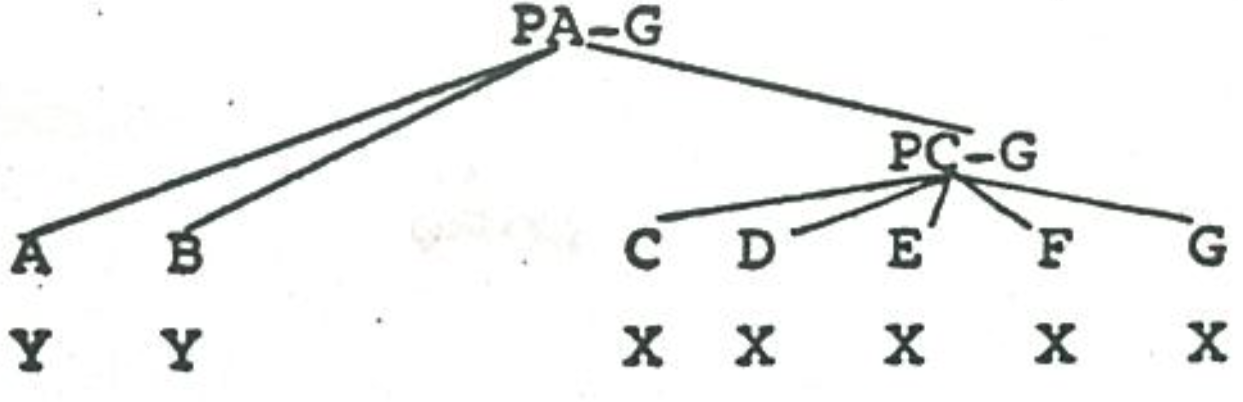
\includegraphics[width=8cm]{illustrations/Clark_1977_tree.png}
\caption{{Tree from \citet[19]{clark1976aspects} illustrating Maximum Parsimony.}}
\label{fig:clark_tree}
\end{figure}

It is important to note that Maximum Parsimony does not take into account branch lengths, only the changes between each node of the tree (regardless of how far apart they are). Furthermore, Maximum Parsimony makes the implicit assumption that the slowest rate of change is the accurate one. This is unlike Maximum Likelihood which does take into account branch lengths and allows rates of changes to be dynamically estimated (more on this in section \ref{sec:asr_methods}.



%Integral to the reconstruction of forms in historical linguistics is \textbf{Maximum Parsimony}. Maximum Parsimony is a method of reconstruction ancestral states (in this case grammatical features of proto-languages) in such a way that there is as few changes as possible from the root to every tip (language). 



\subsubsection{Causes for disagreements: plausibility and Proto-Polynesian}
Reconstruction in historical linguistics also includes judgements of plausibility. This requires some assumptions about what are plausible features to co-occur in language, and which pathways of language change are more plausible than others. For example, it is rare to find a language that has a gender distinction in first person, but not in third (though not impossible; c.f. \citet{wals-44}). If the most parsimonious reconstruction results in a proto-language with many rare features or unusual combinations of features, it may require more investigation. Similarly, changes from certain states to others are assumed to be less plausible. For example, a language going from having no marked dual number on nouns to having trial number would be taken as unusual by most linguists (c.f. \citet[8]{kikusawa_2006_pro_number}). 

Plausibility is important in reconstruction, both in linguistics and in biology. However, this principle is sensitive to differing assumptions and theories. What is more plausible as a reconstructed language or species to one scholar may not be so for another. Besides debates over precise sub-groupings, many arguments in historical linguistics boil down to disagreements about plausibility. This is also true of the different reconstructions of the alignment system of Proto-Polynesian.

\citet{clark1976aspects} disagrees with \citet{hale_1968}, \citet{hohepa_1969}, and \citet{chung1978} on the state of Proto-Polynesian syntax on these grounds. Chung, Hale and Hohepa argue for a theory that is technically less parsimonious, but which they say is more plausible. They posit that Proto-Polynesian had a nominative-accusative case marking system\footnote{Hale, Hohepa and Chung actually suggest three different specific theories for this reconstruction. For a summary of the differences between the proposals, see \citet[247-249]{chung1978}.}. If this was the case, that would mean positing more changes along the tree than if we assumed, as \citet{clark1976aspects} does, that the Proto-Polynesian language was ergative-absolutive. This is due to S\={a}moan and Tongan both having ergative-absolutive marking and both splitting off early (in most accounts of the polynesian tree) from proto-polynesian compared to the rest of the group which most often lacks ergative-absolutive marking.

Chung's critique of Clark's proposal is three-fold: 
\begin{enumerate}[label=(\alph*)]
\item the tree used is not an accurate representation of the language history (there was more interaction between S\={a}moan and Tongan)
\item it is possible that the Proto-language contained variation and was undergoing change that was only fully realised in some of the daughters\footnote{The reason that only some daughter languages exhibit the feature could be due to founder effects (my addition).} 
\item the morpho-syntactical historical process is less plausible
\end{enumerate}

In a review of \citet{clark1976aspects}, Chung writes:

\begin{quotation}
\noindent\emph{Such an approach [as Clark's] relies on the assumption that the subgroups have developed quite independently once they split off from Proto-Polynesian, so that features shared by both must be attributed to the Proto-language. But in fact, both parts of this assumption are too strong. It is well known that the two primary subgroups of Polynesian did not develop totally separately; there was long-standing contact in pre-European times between speakers of Tongic and some Samoic-Outlier languages, as Clark himself notes (p. 27). Further, and more generally, it is simply not true that every feature shared by related languages must have existed in the Proto-language uniting them. Languages are constantly undergoing change; and it is reasonable to suppose that Proto-languages were no different from real languages in this respect. But if this is so, then it is also reasonable that changes begun in a Proto-language may have continued even after its separation into daughter languages. In this way, related languages may come to share a feature which existed only in embryonic form, or not at all, in their common ancestor.}
\end{quotation}
\begin{flushright} \citet[539]{chung1977aspects}  \end{flushright}

This debate contains more twists and turns, with each side arguing for the plausibility of their accounts. In our analysis, we will be using trees that represents the history of the languages in a similar way to Clark, which means the results are sensitive to the same critique by Chung (i.e. not taking into account horizontal transfer between S\={a}moan and Tongan). We are also not able to use plausibility in our computational reconstructions since we do not have access to formalised data on what plausible language profiles or changes are. This is a key difference between computational reconstruction and traditional approaches to reconstruction. Knowledge of plausibility and how to weigh different kinds of evidence against each other is not formalised and cannot be taken into account.

It is possible that with the added information on rates of change and branch length that comes with the Maximum Likelihood approach we are able to approximate some parts of historical linguists' knowledge of plausibility. In that case, we would expect the Maximum Likelihood results to concur more with the predictions by expert linguists. If historical linguists mainly do operate on the same principles of Maximum Parsimony, and/or Maximum Likelihood is not able to approximate plausibility, we would expect the results of Maximum Parsimony to concur more with findings in traditional historical linguistics.

In this study, any instances of conflicting data is evaluated separately from the overall results and will be reported in a separate section. 

%can fall short of reconstructions carried out by classical historical linguists because they are able to take these plausibility considerations into account.

\subsubsection{Reconstruction and subgrouping in tandem}
The processes of subgrouping and reconstruction are done in tandem in historical linguistics. Subgroups are proposed based on shared innovations. In order to determine what is and what is not an innovation, a certain amount of reconstruction is necessary. In order to make reconstructions, some of the tree structure needs to be approximated. Pawley (personal correspondence) notes that most of the subgrouping done in historical linguistics tends to be at the lower level. 
%This can be seen later in this paper in the difference between the Glottolog tree (Fig. \ref{tree_coverage_oceanic_glottolog}), which is based on classical historical linguistics,  and the Gray et al 2009-tree (Fig. \ref{tree_coverage_oceanic_gray}), which is inferred with Bayesian phylogenetic methods using basic vocabulary data. Most of the splits in the Glottolog tree occur close to the tips, whereas the splits are more spread out over the distance between the root and the tips in the Gray et al 2009-tree.

Besides parsimony and plausibility, it is also important to know how to weight evidence when conducting historical linguistics research, in particular when it comes to subgrouping. This is less often discussed explicitly, but it is related to issues of plausibility and is likewise a source of disagreement. It is for example possible that certain data-points are more susceptible to contact-induced change than others, and should therefore carry less weight if we are trying to infer a family tree. This is why items and features that are thought to be particularly stable and unlikely to be borrowed are used in reconstruction and subgrouping (c.f. \citet{pawley_2009_solomons}).

In this paper we are not proposing any new subgroupings, so the problem of weighting evidence is not present in this manner. For the reconstruction of grammatical features, all languages are weighted as equally valuable and we use the tree topologies directly to control for non-independence of datapoints as opposed to careful sampling (c.f. \cite{ross2004morphosyntactic}).
%We are reconstructing grammatical features and this is another area where weighting can be relevant. All languages are weighted the same for the reconstruction, but 

%As was discussed in \ref{sec:dep}, not all data-points are independent of each other and this may be one reason to weight them differently. 

%For example, \citet{wilson_whence} presents a case for Eastern Polynesia (EP) being settled from the so-called ``Northern Outliers'' (i.e. Polynesian languages of Micronesia and the Solomons) by demonstrating shared innovations of lexicon and grammar to the exclusion of Samoa, Pukapuka and Tokelau (which were closer to EP in previous proposals). The paper lays out 73 innovations in support for this theory, and states that there is a lack of shared innovations supporting grouping Eastern Polynesia and the Samoic group together, as had been previously suggested by \citet{pawley1966polynesian}. \citet{wilson_whence} proposes that a more accurate reflection of this data is to group Eastern Polynesian with the Northern Outliers. On the other hand, \citet[53, 61]{pawley1966polynesian} presents two cases where Samoan and some of the Northern outliers shared features to the exclusion of Eastern Polynesia (sing/plural distinctions in indefinite articles and the form of the human number prefix). Besides the sheer number of data-points, it is clear that historical linguists also weight different pieces of information differently. Without an internalised in-depth knowledge of these matters, it is difficult to know how to evaluate the support for these conflicting theories of the origins of Eastern Polynesian communities. Is it as significant that the Northern Outliers and Eastern Polynesian languages shared a word for a certain kind of fish (\emph{*kamakama}) as the fact that they have also, as a group, added an \emph{o-} to the Proto-Polynesian root \emph{*fia} (want) \citep{wilson_whence}? 

%In this paper we are not proposing any new subgroupings, so the problem of weighting evidence is not present in this manner. We are, however, reconstructing grammatical features and this is another area where weighting can be relevant. All languages are weighted the same for the reconstruction, but 

%The tree structure and the method (Maximum Parsimony or Maximum Likelihood) determines the reconstruction. This can be compared to weighting evidence from oversampled areas/subgroups less when reconstructing. 

% \citet[135]{marck2000} also presents the case that the Northern Outliers are most closely related to Tuvaluan.

%It is clear that considerable experience and meticulous considerations are needed in order to make these judgements and interpret the results of these papers appropriately. This entails long periods of training and familiarisation with the method in practice and the particular languages in question. \citet[721-731]{blust2013austronesian} suggests that we should bring in non-linguistic evidence to bear on these theories as well. How would a settlement from the Northern Outliers be achieved materially? By finding supporting or conflicting evidence from other disciplines, we can make more robust predictions 

%For full disclosure, both of the trees used in this study (Glottolog 4.0 and \citet{grayetal_2009}) group EP closer to the Northern Outliers than to Samoan, and it is becoming more accepted. 


\subsection{Characteristics of language structure as data}
\label{diff_lexi_str}

The Comparative Method is most often applied to vocabulary, but it can also be applied to grammatical morphemes and features. \citet{crowley1985common} for example traces the history of a common noun phrase marker \emph{*na/*a} in Oceanic languages using the Comparative Method. 

The data in this paper does not track specific forms, as is common when reconstructing Proto-languages in historical linguistics (c.f \citet{pawley1973some, crowley1985common, evans2003study}). Instead we use binary features of a typological questionnaire which tracks large part of ``core" grammar (see section \ref{asr:sec:GBcoverage}). This section outlines some crucial differences between structural data and the kind of data that is typically used in historical linguistics in relation to the present study.

The kind of data used in grammatical reconstruction in historical linguistics differs from what we find in linguistic typological questionnaires such as Grambank. \citet{crowley1985common}, \citet{clark1976aspects}, and other scholars whose work we will compare to our results in this paper, typically apply the comparative method to specific formal expressions of structural features (the \emph{na} article, \emph{-Cia} suffix, \emph{faka-} prefix etc). They take into account fossilised forms (the common noun marker \emph{-a} fusing to roots in Paamese \citep[141]{crowley1985common}) and related meanings (the hypothesis of \emph{-Cia} changing from a transitivising suffix to a marker of passive voice (\citet{hale_1968, hohepa_1967, hohepa_1969, chung1978} and \citet{jonsson1998}). The Grambank dataset, however, (as many other typological surveys) only considers productive patterns and does not include information on specific formal expressions of grammatical phenomena.

Two languages can be coded identically for a structural feature in a typological questionnaire due to entirely different reasons and without being related. For example, Koasati [koas1236] of Louisiana, USA, and Mokilese [moki1238] on Mwoakilloa in the Federated States of Micronesia are both coded as having a construction for predicative possession of the type ``Topic'' by \citet{wals-2011-117}. However, they belong to entirely different language families and different parts of the world. This is unlike cognacy data, where the fact that two languages have cognates in common is direct evidence of relatedness.

An example of the differences between the structural data used in classical historical linguistics and typological questionnaires is the definite marker in Oceanic. \citet{crowley1985common} investigates common noun phrase markers\footnote{This term is more or less identical to a pre-nominal definite/specific article.} in Oceanic and finds that in many languages there is a reflex of proto-Oceanic \emph{*na/*a}, but that in some languages there is another marker with a different origin (M\={a}ori \emph{te} for example). In Crowley's study, languages where there is no common noun phrase marking whatsoever and those with a marker which is not cognate with \emph{*na/*a} are both included in type 1 (see Fig.~\ref{fig:crowley_map}). These languages are contrasted with those that have retained some kind of reflex of \emph{*na/*a} (type 2-4 in Fig.~\ref{fig:crowley_map}). This means that we can distinguish languages which have retained the proto-form from those that have not, but not languages which have a common noun phrase marker from those that do not.

\begin{figure}
\centering
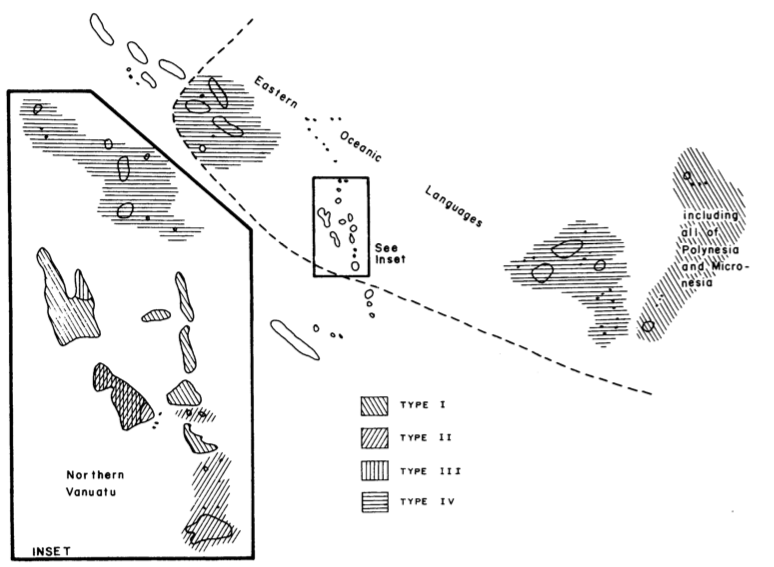
\includegraphics[width=8cm]{illustrations/crowley_1985_map.png}
\caption[Map of four different types of common noun phrase markers in Oceanic from Crowley(1985).]{\textbf{Map of four different types of common noun phrase markers in Oceanic from \citet[162]{crowley1985common}. Type 1: absence of common noun phrase marker or marker is not a reflex of \emph{*na /*a}, type 2: non-productive system involving a reflex of \emph{*na /*a}, type 3: productive marking involving \emph{*na /*a} as a prefix that is regularly separable from the noun and type 4: productive marking involving \emph{*na /*a} generally existing as a free-standing marker.}}
\label{fig:crowley_map}
\end{figure}

In contrast, the corresponding feature in Grambank is `GB022: \emph{Are there prenominal articles?'} (see Fig.~\ref{fig:gb022_map}). Languages that have \emph{te} (like M\={a}ori) or reflexes of \emph{*na/*a} as articles before the noun both count as ``yes'' (1) for GB022 and those that have no prenominal marker as a ``no'' (0). This Grambank feature splits Crowley's type 1 into two categories, and combines all the languages with reflexes of \emph{*na/*a} and \emph{te} (or other markers) into one category. We can now distinguish those that have a pre-nominal article from those that do not, but we cannot tell apart those which have retained the proto-form from those which have not. Since many reconstructions of grammar in historical linguistics rely on particular forms, this is an important difference. This does not matter for features such as word order.

\begin{figure}
\centering
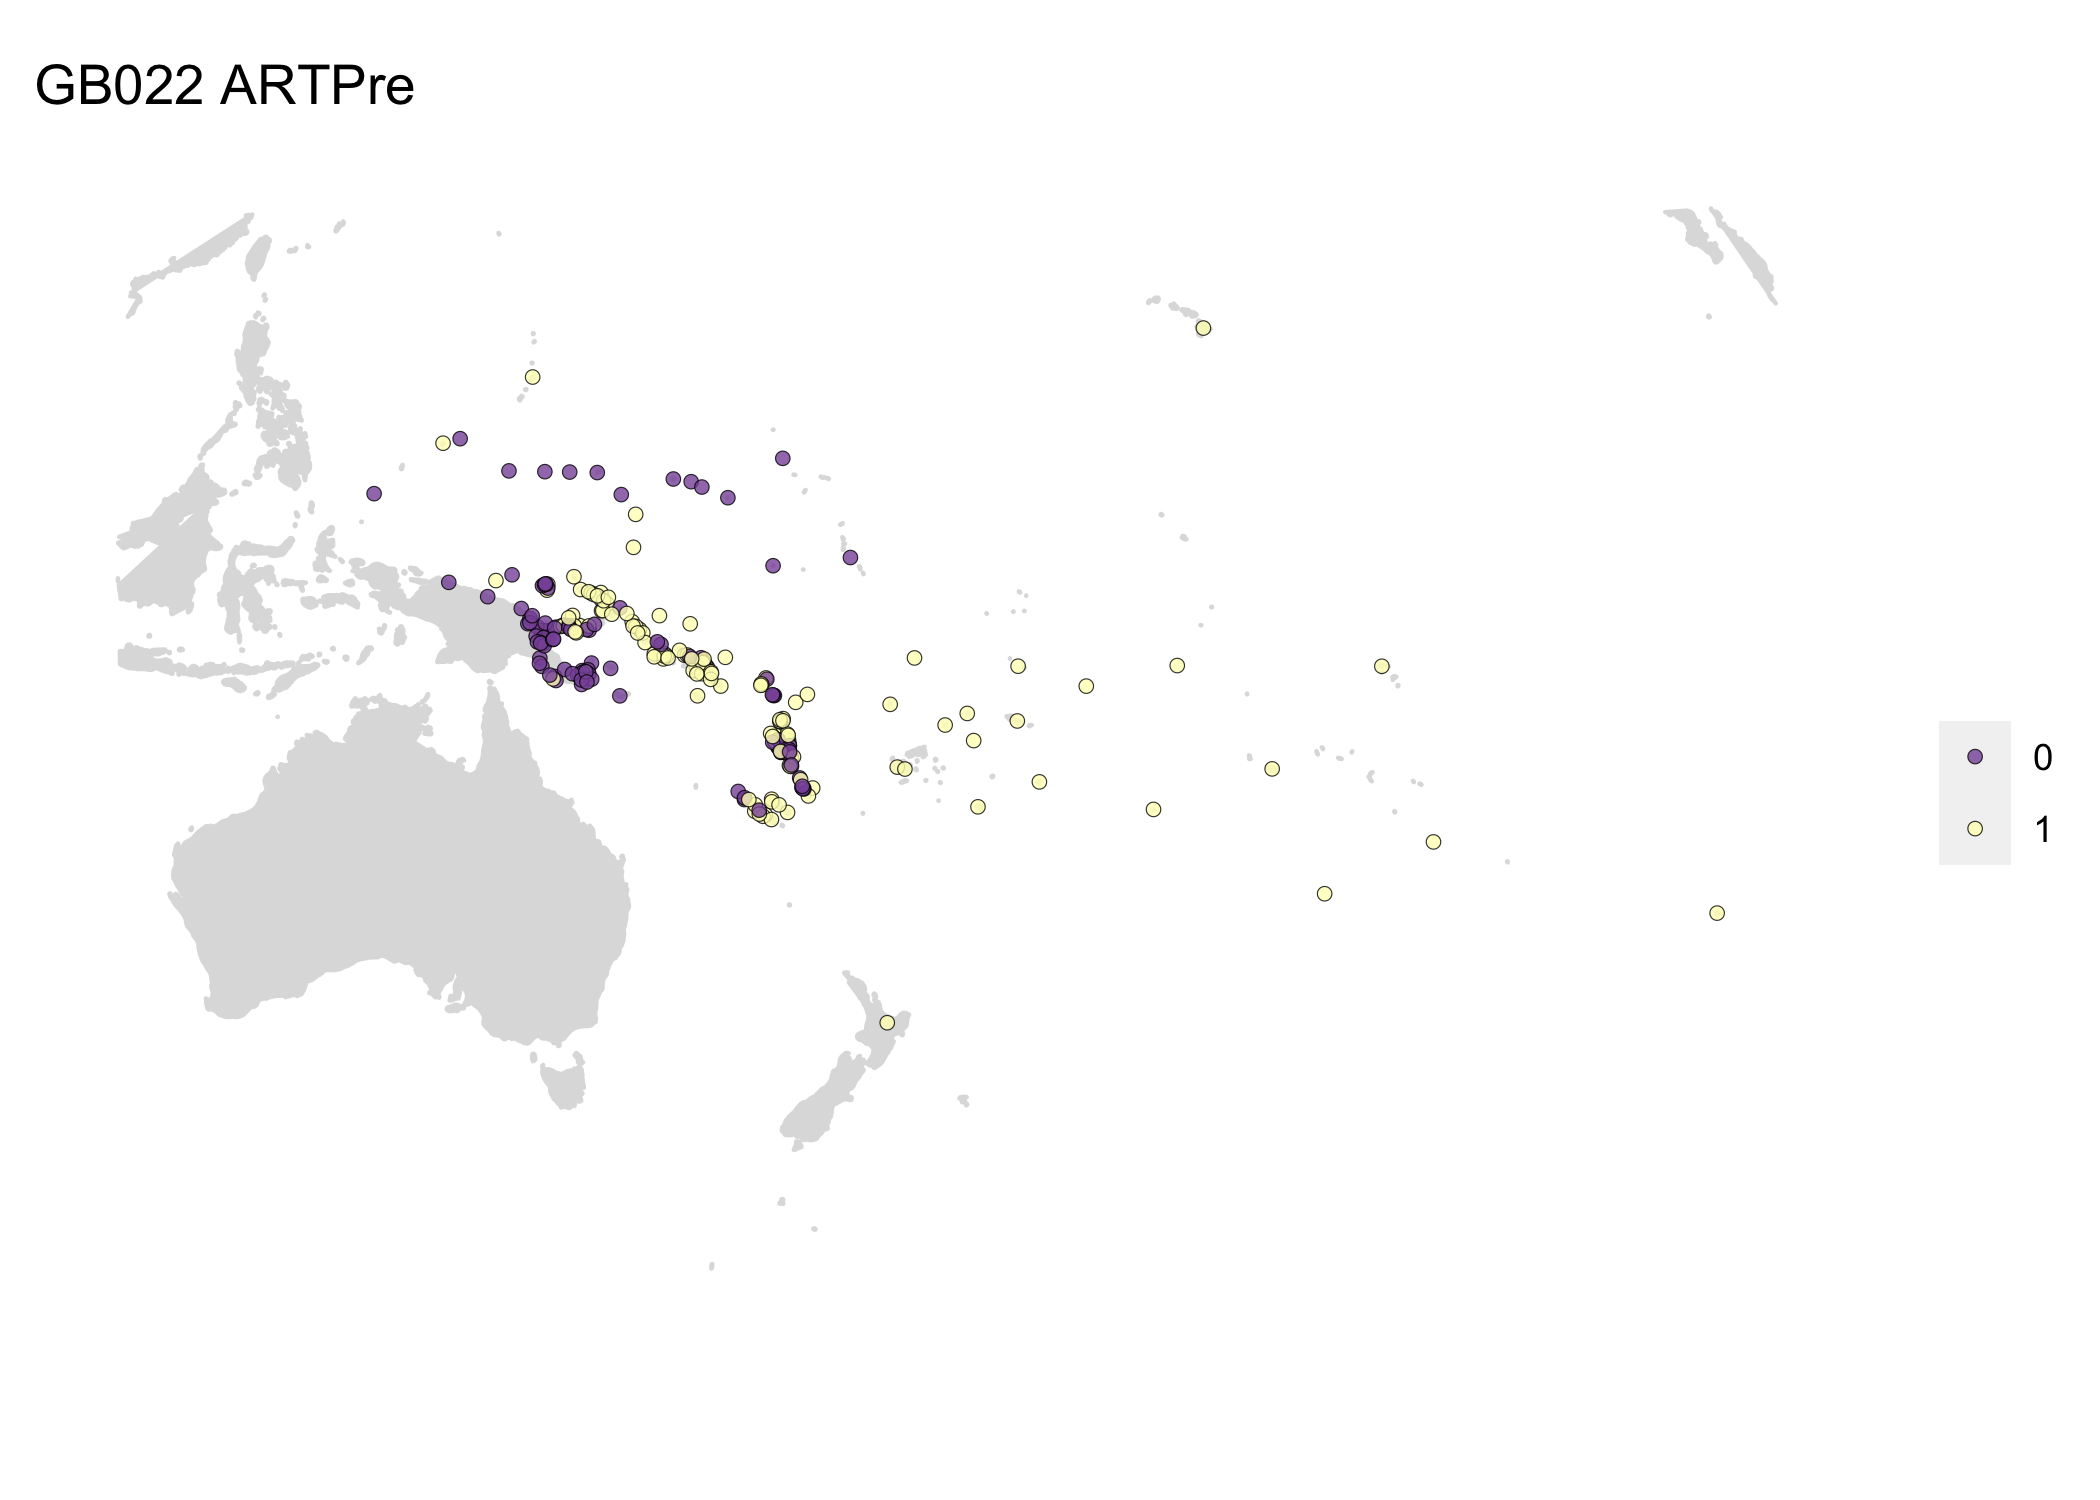
\includegraphics[width=20cm]{../code/output/coverage_plots/maps/map_GB022.png}
\caption{{Map of Austronesian languages for GB022 \emph{Are there prenominal articles?} Yellow = ``yes", purple = ``no".}}
\label{fig:gb022_map}
\end{figure}

While reconstruction in traditional historical linguistics often relies on particular grammatical morphemes, the data in this study is composed of abstract features such as ``is a grammatical distinction made between X and Y?". While this is worth to keep in mind, it should also be noted that it is possible that such abstract features track something beyond the particular forms. \citet[503]{ross2004morphosyntactic} notes that a particular structure of the pronominal system of Mokilese is maintained, despite the formal markers being continuously replaced. He argues that there are discourse related reasons for maintaining this system and that the interaction between this construction and the rest of the grammar is such that the distinction is maintained. When particular markers are lost in this system, new ones appear in their place. He also notes that Goddard has observed similar patterns in Algonquian languages \citep{goddard1993algonquian}. 

%Furthermore, it is possible that due to the interconnectedness of structural features related languages can develop similarily without 
%Related languages may also show similarity due to inheritance, even if the relevant state was not present in the ancestor, as the quote from \citet{chung1977aspects} earlier continues:

%\begin{quotation}
%\noindent\emph{[I]t is also reasonable that changes begun in a Proto-language may have continued even after its separation into daughter languages. In this way, related languages may come to share a feature which existed only in embryonic form, or not at all, in their common ancestor}\footnote{This idea is important to a particular hypothesis about Proto-Polynesian syntax, because according to \citet{chung1978} Proto-Polynesian was accusative and Tongan and S\={a}moan both developed ergativity semi-independently while the Eastern Polynesian languages (which are more closely related to S\={a}moan than to Tongan) did not develop this feature.}.
%\end{quotation}
%\begin{flushright} \citet[539]{chung1977aspects} \end{flushright}
%
%This theory proposes that the conditions for developing a certain feature may have been present in the ancestral language even if the feature itself is absent. It is therefore likely that the daughter languages would develop it even if they were isolated from each other, because they have inherited the prerequisites for developing the feature. This is similar to what is known in the literature on cultural evolution as ``preadaptation'' \citep{scott2010language}. One might say that the seed is sown already in the parent language, and that as a result its daughter languages will likely turn out a certain way.
%
%This ties in with the dependencies of features, insofar as dependencies are representations of features ``moving as a group'' through time. If some of these features are reliable ``early movers'', one could use them to predict certain developments in daughter languages. This theory aligns well with a view of language as a system where everything neatly fits (``La langue est \emph{un système où tout se tient}'' [language is systematic / a system where everything fits], Saussure \citep{koerner1997notes}). This is in contrast to the view by, among others, \citet[328]{bloomfield1933language} who stated that \emph{every word has its own history}. It is likely that systematic effects like these are more probable in structural data than in lexical data.
%
%However, in this analysis we are investigating each feature separately so it is not possible to derive information about features co-evolving. It is also difficult for the algorithm \emph{not} to reconstruct a certain state in the parent language, if the majority of daughter languages possess it. This is one instance where knowledge of plausible paths and profiles of languages from classical linguistics may contribute information that is, so far, not possible to retrieve using computational means.

%In summary, the comparative method of historical linguistics involves Maximum Parsimony coupled with information on plausibility. It is not possible in computational reconstruction to take plausibility into account since it has not been formalised. The kind of data typically used in reconstruction of grammar in historical linguistics concerns specific forms, whereas the data for this paper is structural features.

\section{Material and methods}
\subsection{Computational phylogenetic methods}
\label{sec:asr_methods}

In this study, we will be reconstructing the presence or absence of structural features in proto-languages of the Oceanic subgroup using Maximum Parsimony and Maximum Likelihood. This section gives a brief overview of the methods, further technical details concerning the precise application can be found in the supplementary material \ref{supp:tech_details}. For an extensive comparison of different methods of ancestral state reconstruction and their advantages, see \citet{joy2016ancestral}.

As discussed earlier in section \ref{sec:ars:metod:hist}, \textbf{Maximum Parsimony} finds the set of ancestral states that result in the fewest number of changes between nodes. Maximum Parsimony is intuitively simple. We saw in the previous section an example of how it can play out in a small tree. While the principle of ``Maximum Parsimony'' is practised in traditional historical linguistics as a part of the Comparative Method, it should be noted that they rarely use the term \emph{per se}, but rather the description of ``fewest number of changes along the tree'' (along with the other two principle of plausbility of the reconstructed language and of the changes).

Maximum Parsimony may be simple and intuitive, but it is not without its critique. Part of the critique is that it does not take into account branch lengths in the tree (the distance between splitting events). Furthermore, Maximum Parsimony necessarily assumes that the solution that posits the slowest possible rate of change is also the most probable one. This is not necessarily a valid assumption, some features may evolve at a faster rate than Maximum Parsimony predicts. Both of these disadvantages are addressed in the second method we will be applying: Maximum Likelihood.

%The second method which will be applied in this study is that of \textbf{Maximum Likelihood}. 
Ancestral state reconstruction using Maximum Likelihood posits the most likely ancestral state distributions based on the overall probabilities given all the nodes in the tree and all branches. This approach does not assume that the slowest rate of change is the most probable one. If, for example, the distribution of values at the tips is very scattered, with sibling pairs frequently having different profiles, Maximum Likelihood will infer that the feature has a high rate of change and use that information when positing ancestral states as well. The Maximum Likelihood algorithm assigns probabilities of state changes and distributions based on branch lengths. A mutation along a shorter branch is given more weight in the likelihood calculations than if it occurred in a longer branch. Furthermore, reconstruction using Maximal Likelihood allows us to use a model of change where we do not assume that the rates for losses (1$\rightarrow$0) are equal to the rate of gains (0$\rightarrow$ 1). In this study, we use an ``All Rates are Different" (ARD) model, which allows for the rate of loss and gain to be different. 

It is not possible for the computational implementation of Maximum Parsimony to take into account branch lengths, nor can it assume anything but the slowest rate of change or posit different rates for losses and gains. It is however possible that the Comparative Method in historical linguistics estimates something similar when they take into account the ``plausibility of the changes posited'' and that this is picked up by the reconstruction by Maximal Likelihood. It is possible that scholars of historical linguistics take length of time into account, for example, or assume that a loss is more likely than a gain for a given feature. In this study, we compare Maximum Parsimony and Maximal likelihood reconstructions to the Comparative Method. If the results from the Comparative Method are more similar to that of Maximum Likelihood then that is is possible that the ``plausibility of changes posited'' is indeed operating along similar lines as Maximum Likelihood by taking branch length into account and assuming varying rates of change.

%The third method employed is \textbf{Stochastic Character mapping}. This method was proposed by \citet{huelsenbeck2003stochastic} and is an extension of an approach suggested by \citet{nielsen2002mapping}. 
 

\subsection{Evaluation of methods}
We will evaluate the computational methods by comparing them to a gold standard of reconstructions done by historical linguists using the classical Comparative Method approach. Concordance is measured both by the number of agreements between each method divided by the total amount of reconstructions (``accuracy'') and F1-scores. A F1-score is the harmonic mean of the precision and recall\footnote{Precision is True Positives divided by True Positives + False Positives, recall is True Positives divided by False Negatives + True Positives. F1-score = 2 * ((precision*recall) / (precision + recall)) \citep{van1979information}.} of the result of each method as compared to a gold standard \citep[133]{van1979information}. For both measures of concordance, 0 is the worst possible score and 1 the best. 

In a similar study of ancestral states of cognate classes, \citet{jager2018using} compared three different methods of ancestral state reconstruction for lexical data (cognate classes): Maximum Parsimony, Maximum Likelihood and Minimal Lateral Networks. They found that reconstructions using Maximum Likelihood performed ``better'', in the sense that it more often predicted the same values as their gold standard compared to the other two methods\footnote{ The gold standard consisted of reconstructions by historical linguists, and it should be noted that it is possible that this standard may contain errors as well.}. 

\citet{jager2018using} describe the general performance of all the computational reconstruction methods they used as ``poor''. . The highest F1-score was 0.79 (Austronesian language sample, Maximum Likelihood), and the worst was 0.44 (Indo-European, Minimal Lateral Networks). 

\citet{jager2018using} only evaluated the methods using the F1-score, but because this ignores the amount of True Negatives we will also measure a more plain accuracy score. 

In addition to these two concordance scores we will also calculate how much better each method does compared to just counting which is the most common vale of a feature in the daughter languages. As we learned in section \ref{sec:ars:metod:hist}, simply relying on frequency and not taking the tree structure into account can lead us astray. Whether we prefer Maximum Parsimony, Maximal Likelihood or another approach to reconstruction it should be the case that actually taking the tree structure into account is the more sound methodology. We expect that both methods has a higher degree of concordance with the findings in historical linguistics compared to only counting which value is most common.



In this section we compare how often the computational reconstructions are in concordance with those made by historical linguists. For each feature, the algorithm predicts a distribution of the two states (presence and absence) for every ancestral node. If the distribution is majority presence (more than 60\% of the ancestral state is ``1'') it is registered as ``Presence''; if less than 40\% presence it is registered as ``Absence''. If the ancestral state is between 40-60\% of either state, the prediction is registered as ``Half/Half''. If the reconstruction of a feature by experts for that ancestral node was ``Presence'' and the algorithm did predict presence with over 60\%, it is a ``True positive'', and so on. Table~\ref{example_HL_prediction_table_true_positives} illustrates how the results are calculated.

\begin{table}[H]
\centering
\caption{Table illustrating how the results of ancestral node predictions are calculated.}
\label{example_HL_prediction_table_true_positives}
\begin{tabular}{|l|l|l|l|l|l|l|l|}
\hline
\textbf{Finding in historical linguistics} & \textbf{Prediction by MP or ML} & \textbf{Result} \\ \hline
Presence & >60\% Presence & True Positive \\ \hline
Presence & >60\% Absence & False Negative (type 2-error) \\ \hline
Absence & >60\% Absence & True Negative \\ \hline
Absence & >60\% Presence & False Positive (type 1-error) \\ \hline
Presence & 40-60\% Presence/Absence & Half/Half\\ \hline
Absence & 40-60\% Presence/Absence & Half/Half \\ \hline
\end{tabular}
\end{table}

In order to evaluate the results, we need to calculate a concordance score per method and tree. \citet{jager2018using} use the F1-score (harmonic mean between precision and recall) in their study of how computationally reconstructed lexical proto-forms compare to those reconstructed by historical linguists.  For example, if for a given proto-language there are 60 features reconstructed by experts and the algorithm result is 10 True Positives, 10 False Positives, 10 True Negatives, 10 False Negatives and 20 ``Half/Half'' then the F1-score is 0.5 (recall = 10 / (10+10) = 0.5, precision = 10 / (10+10) = 0.5 and F1-score = 2 *((0.5*0.5) / (0.5 + 0.5) = 0.5)). Note that the F1-score disregards True Negatives and Half /Half-results.

F1-scores will be reported because they are insightful and have been used in similar studies. However, the F1-formula ignores the amount of True Negatives and Half/Half results. Therefore, in addition we will also calculate a simpler concordance score; how many concordant predictions did the algorithm make given all the predictions it made (aka ``accuracy'')? For example, if for a given proto-language there are 60 features predicted by experts with the same distribution of results as in the example above, then the concordance score would be (10 + 10)/40 = 0.5. We can also include the Half/Half-predictions, awarding 0.5 points for at least not strongly predicting a false value. In that case, this example has a concordance score of 0.5 ((10 + 10 + (20/2)) / 60). These scores all reflect different ways of assessing concordance and will give different perspectives on our results and how our algorithms are performing. %Features where there were more than half of the data-points missing in the tree were not to be included. hankfully there were no occurrences of this.

\subsection{Data}

\subsubsection{The Grambank-dataset}
\label{asr:sec:GBcoverage}

The data for the study is taken from the Grambank-project \citep{grambankwebsite}. The Grambank dataset consists of 195 structural features which have been coded by a large group of research assistants for over 2,000 languages. This dataset includes 276 Oceanic languages. 

%The Grambank project is part of the Glottobank consortium, which is a collaboration between the Max Planck Institute for the Science of Human History in Jena (MPI-SHH), the Australian National University, the Australian Research Council's Centre of Excellence for the Dynamics of Language and the University of Auckland. The project is led by a team of senior linguists (Russell Gray, Simon Greenhill and Quentin Atkinson) and employs student assistants as coders in Kiel, London, Canberra, Uppsala and a few other locations. Coders who have been contributed significantly to the database are included as co-authors of the upcoming release paper \citep{grambank_release}, alongside other contributors. I have personally participated in this project as a coder and as a coordinator.

%The aim of Grambank is to provide a consistently coded set of structural features of the world's languages for research questions relating to history, complexity and more. The dataset will be published openly. 
 
%The Grambank dataset builds on previous typological work by \citet{dunnetal2005, dunn2008, reesinketal2009, dunnreesink2012} and \citet{ntswebsite}. The project has a global focus and the aim is to include all languages in the world that are described for their core grammatical structure. 

% In the work by Dunn, Reesink and colleagues, they were particularly focussed on languages of Oceania and Australia and the prehistory of migrations and contact there. The Nijmegen Typological Survey-project \citep{nts2014, ntswebsite} on the other hand was focussed on African languages.

The questionnaire contains 195 questions and covers what are often called the ``core domains'' of traditional grammatical description: word order, possession, negation, tense, aspect, mood, deixis, interrogation, comparatives and more. Features are included in the questionnaire if it is likely that it is possible to answer them for the majority of the world's languages which are at least described in a grammar sketch (approx 4.000 languages). This means that rarer features are not included. The full questionnaire is found in appendix \ref{Grambank_features}. 

The Grambank dataset is coded by student and research assistants under the supervision of expert linguists. For more details on the coding workflow of Grambank, see \citet{slingerland2020coding}. For further details on the dataset, see Supplementary Material ~\ref{supp:dataset_details}.

%It is crucial in a cross-linguistic survey of this kind that the features are applied consistently across all languages of the sample. Within the Grambank-project, we strive towards a high level of consistency between coders. There are many coders employed and we have established work-flows to ensure that the features are applied consistently across languages. New coders are trained in the workflow and linguistic definitions through collaborative coding. Each feature in the questionnaire is accompanied by a helpful and pragmatic definition in a wiki-page. Each feature is also associated with a ``patron'', an expert linguist assigned to a set of features who has the final word should any further clarification be needed or disagreements arise. There are seven patrons in the project: Alena Witzlack-Makarevich, Harald Hammarström, Hannah Haynie, Jeremy Collins, Jay Latarche, Jakob Lesage and myself. All coders in the project are able to converse with each other and patrons through GitHub, an online platform for project coordination and code collaboration. When we are unable to make a coding decision with sufficient confidence, the data-point is marked as ``?''.


\subsubsection{Data coverage} 
This study is focussed on the Oceanic subgroup of the Australasian language family. The Oceanic subgroup covers almost all languages in Remote Oceania, with the exceptions of Chamorro and Palauan, and large parts of Near Oceania. Fig.~\ref{Oceanic_map} from \citet[2]{protooceanicvol5} shows the extent of the major subgroups of the Austronesian language family, with Oceanic covering the largest surface area. Following the language classification of Glottolog 4.0 \citep{glottolog40}, there are 522 languages in the Oceanic subgroup.

%For the purposes of this study, we have used the definition of the Oceanic subgroup from Glottolog 4.0  This gives a total of 521 Oceanic languages.

\begin{figure}[h]
\centering
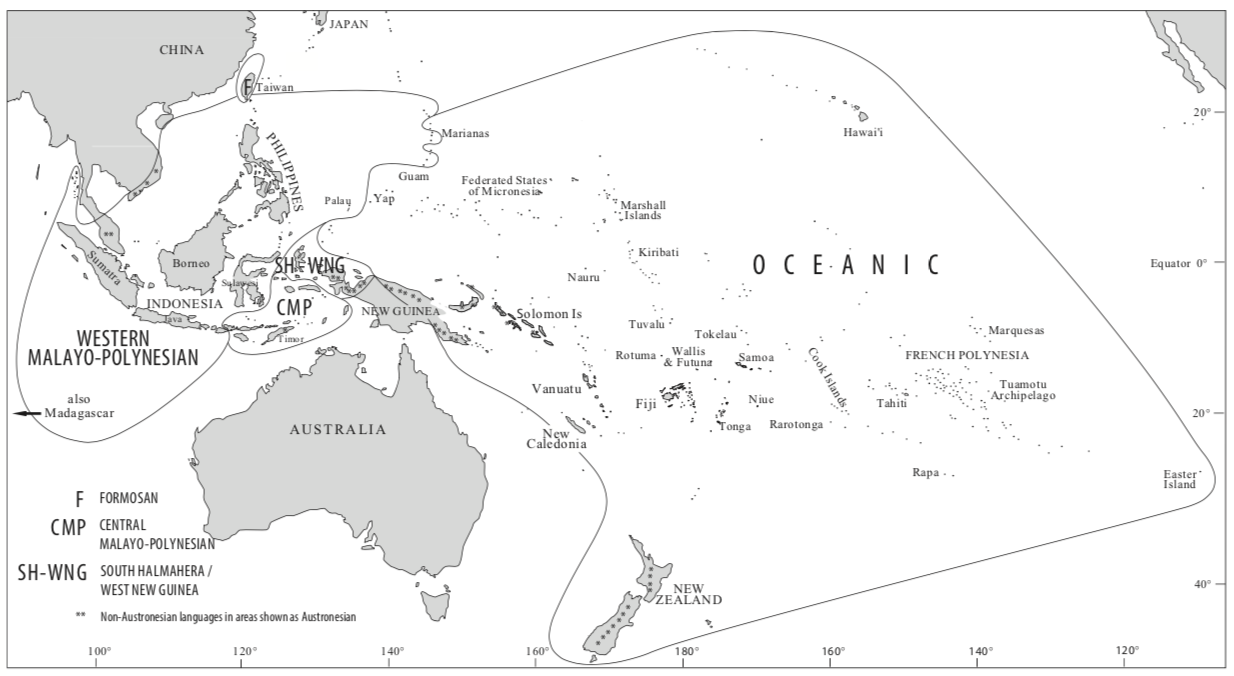
\includegraphics[width=\textwidth]{illustrations/ross_pawley_osmond_protooceanic_vol5.png}
\caption{{Map of the Austronesian language family and major subgroups, from \citet[2]{protooceanicvol5}.}}
\label{Oceanic_map}
\end{figure} 

Not all languages of the Oceanic subgroup are described grammatically, but out of those that are nearly all are coded for the Grambank typological questionnaire. Table~\ref{GB_coverage_table} shows the coverage of Oceanic languages in the dataset. Of all the languages in the subgroup, there are 261 languages that have been documented in descriptive works such that we are able to answer our questionnaire. 241 languages are currently too poorly described for us to include them in the database. As has been discussed before, it is not always possible to fill in all the features for every language. Nineteen of the Oceanic languages that are included to date are less than 50\% completed. This can be due to lack of access to descriptive work, or that the content of the descriptive work doesn't cover the necessary domains in enough detail for the coders to answer enough questions. The map in Fig.~\ref{GB_austro_coverage} shows the same coverage information, with languages coded for their data coverage status.


\begin{table}[h]
\caption{{Table showing coverage of Oceanic languages in Grambank per island group, total Oceanic languages}}
\label{GB_coverage_table_island_group}
\centering
\begin{tabular}{|l| p{2.7cm}| p{2.7cm} | p{2.7cm} |p{2.7cm} |}
  \hline
\textbf{Island group} & \textbf{\cellcolor{hedvig_orange!50}{No grammar}}  & \textbf{\cellcolor{hedvig_blue!50}{Grammar exists, but language not in Grambank (yet)}} &\textbf{\cellcolor{hedvig_lightgreen!50}{Less than half of the features covered in Grambank}} & \textbf{\cellcolor{hedvig_darkgreen!50}{More than half of the features covered in Grambank} } \\ 
  \hline
Bismarck & 5 & 0 & 7 & 43 \\ 
  Central Pacific & 11 & 0 & 1 & 33 \\ 
  Central Vanuatu & 42 & 0 & 1 & 48 \\ 
  Interior New Guinea & 11 & 1 & 0 & 3 \\ 
  Micronesia & 6 & 0 & 1 & 16 \\ 
  N Coast New Guinea & 77 & 5 & 3 & 16 \\ 
  New Caledonia & 18 & 1 & 0 & 14 \\ 
  Northern Vanuatu & 9 & 0 & 0 & 5 \\ 
  S New Guinea & 36 & 8 & 1 & 21 \\ 
  Solomons and Bougainville & 25 & 1 & 4 & 30 \\ 
  Southern Vanuatu & 1 & 0 & 0 & 8 \\ 
  Temotu & 3 & 0 & 2 & 5 \\ 
  Total & 244 & 16 & 20 & 242 \\   
\end{tabular}

\end{table}

\begin{sidewaysfigure}
\centering
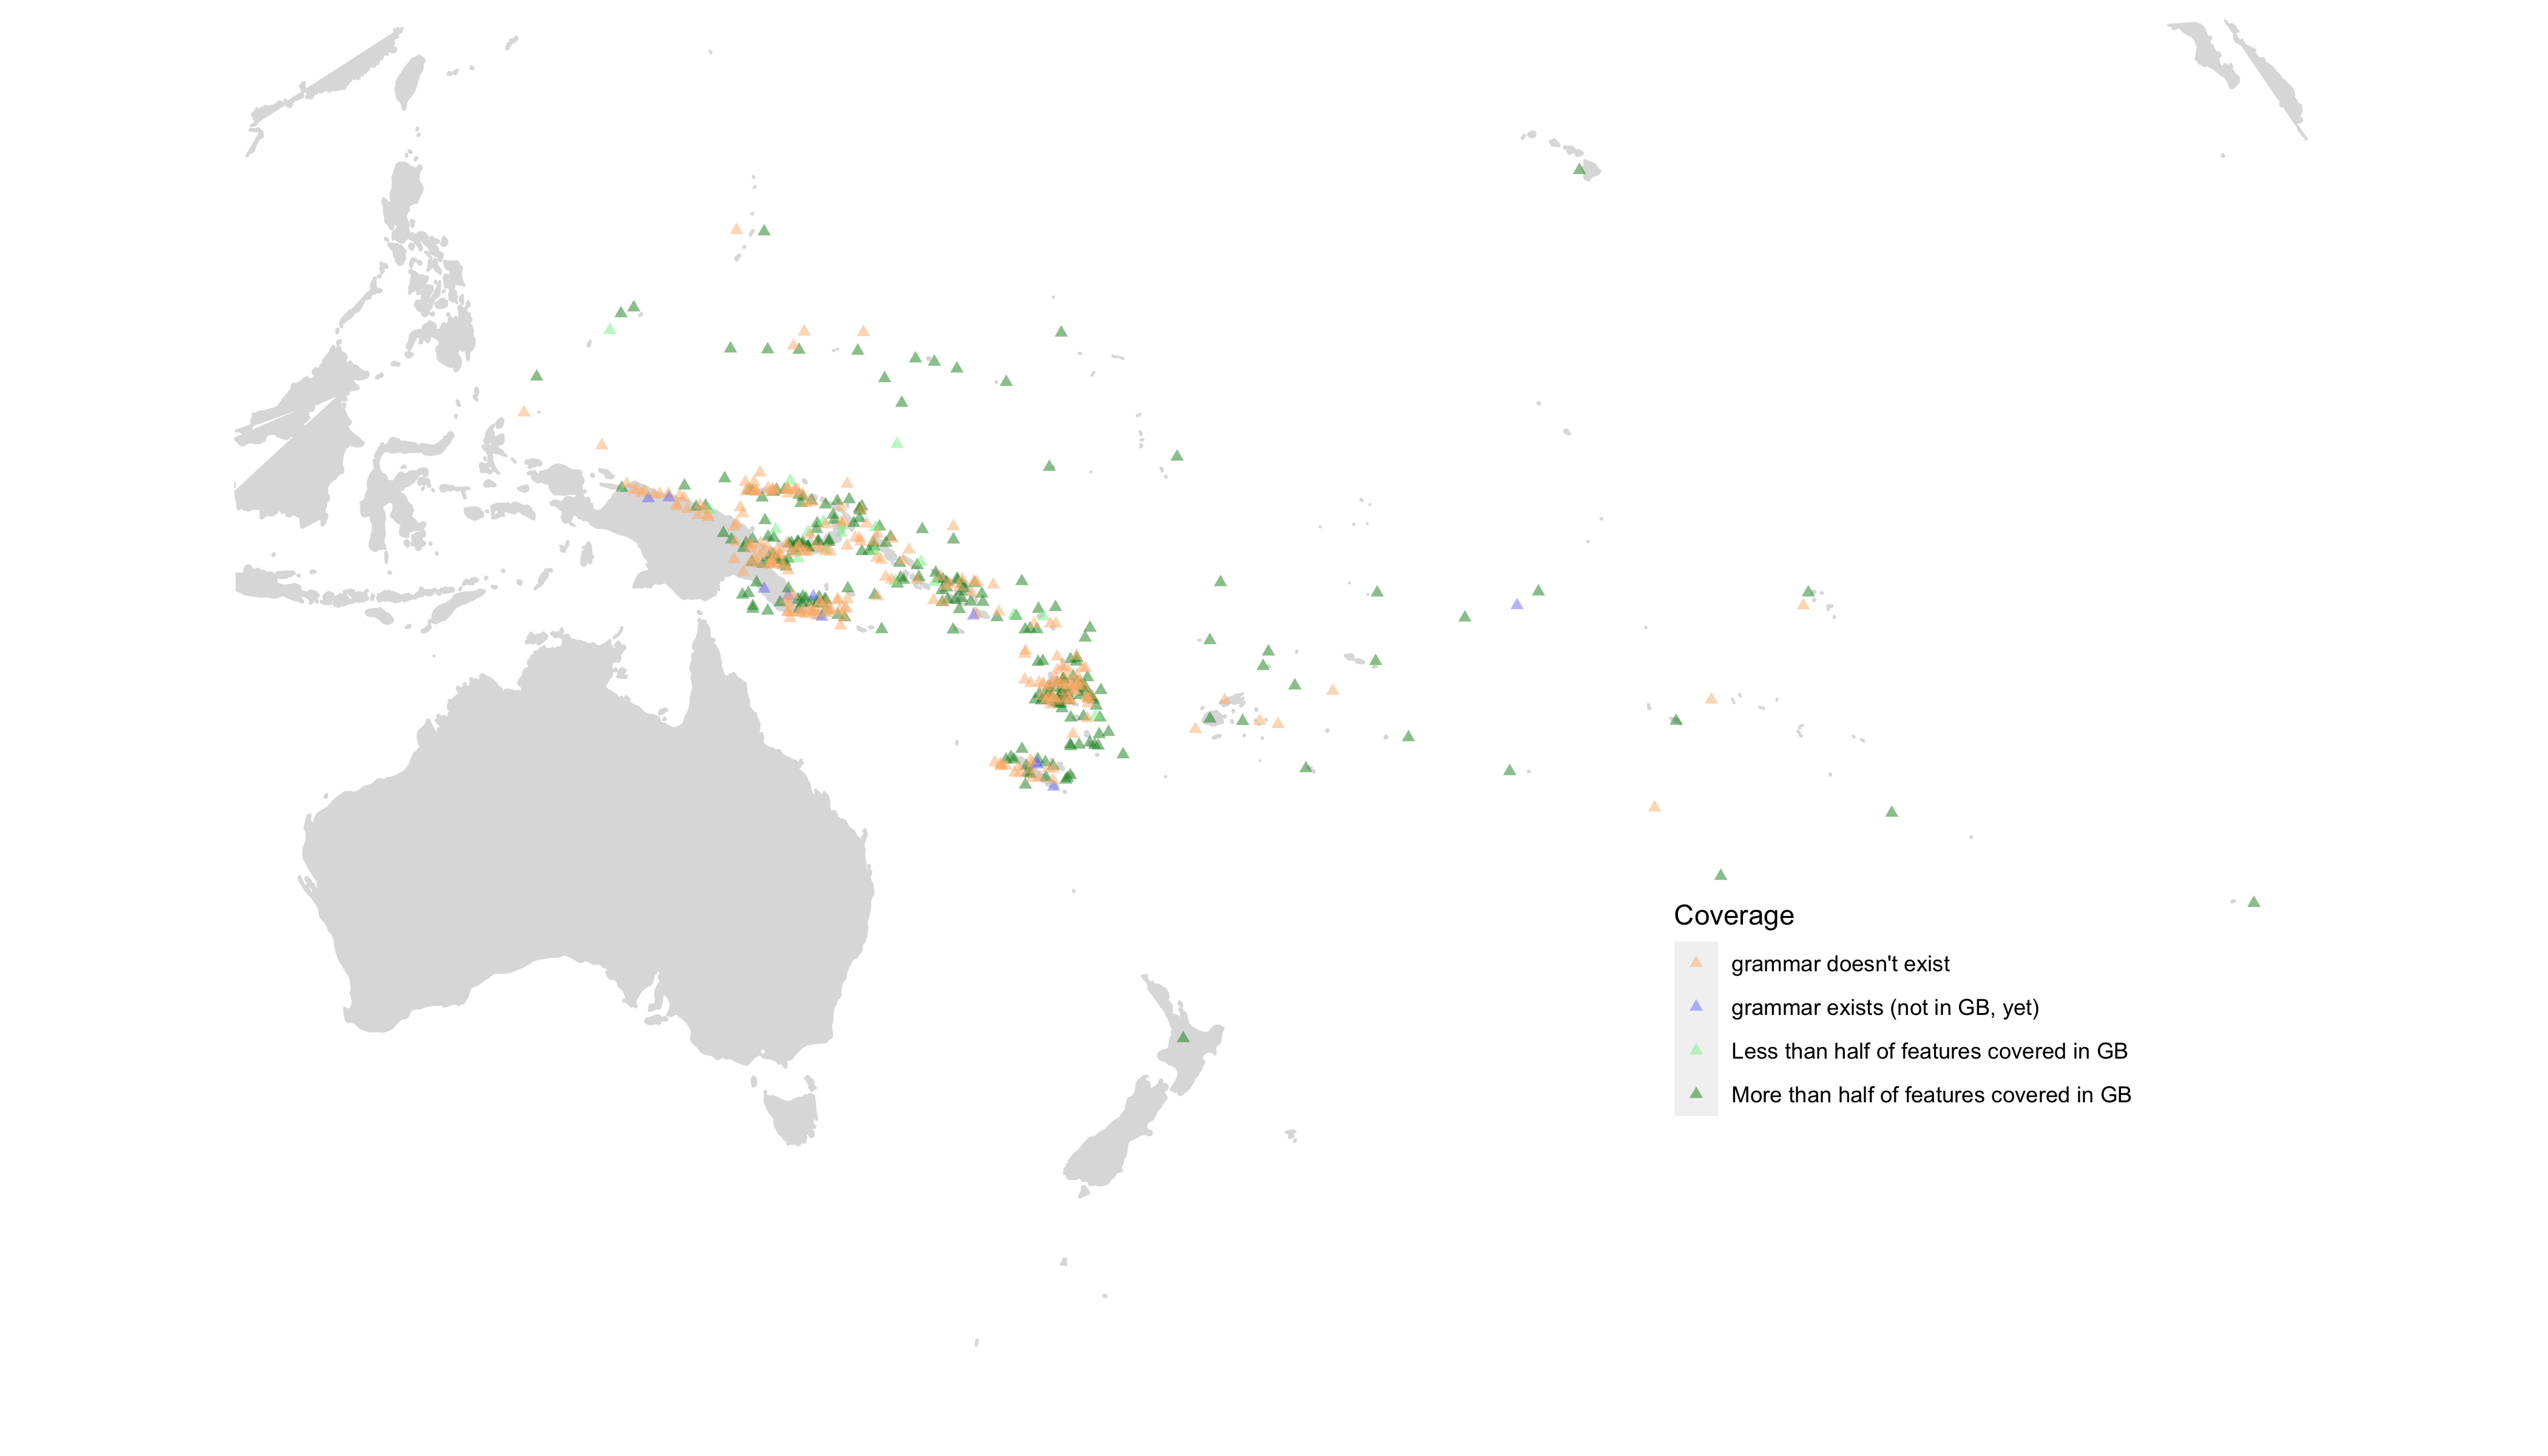
\includegraphics[width=\textwidth]{../code/output/coverage_plots/maps/coverage_map_oceanic.png}
\caption{{Map of Oceania, with Oceanic languages coloured for their coverage in Grambank.}}
\label{GB_austro_coverage}
\end{sidewaysfigure} %#update

The coverage of Grambank data for the Oceanic subgroup is in general better in the east than in the west. However, since we control for genealogical relatedness through the distance control approach, this is less of a problem for our methodology than if we were using traditional probability sampling (c.f. \citet{ross2004morphosyntactic}).




\subsubsection{The trees}
The tree phylogenies used in this study are: a) the Maximum Clade Credibility Tree (MCCT) from \citet{grayetal_2009} b) a random sample of 100 posterior trees from the same source and c) the tree from Glottolog 4.0 \footnote{The tree of Glottolog 4.0 is based on work by \citet{blust_2009, blust_2014} and \citet{blust_chen_2017}.}. 

Figure ~\ref{tree_coverage_oceanic_gray} and Figure ~\ref{tree_coverage_oceanic_glottolog} shows the Grambank coverage of languages over the phylogenies from the Gray et al 2009-MCCT-tree and the Glottolog-tree respectively. 

\begin{figure}[H]
\centering
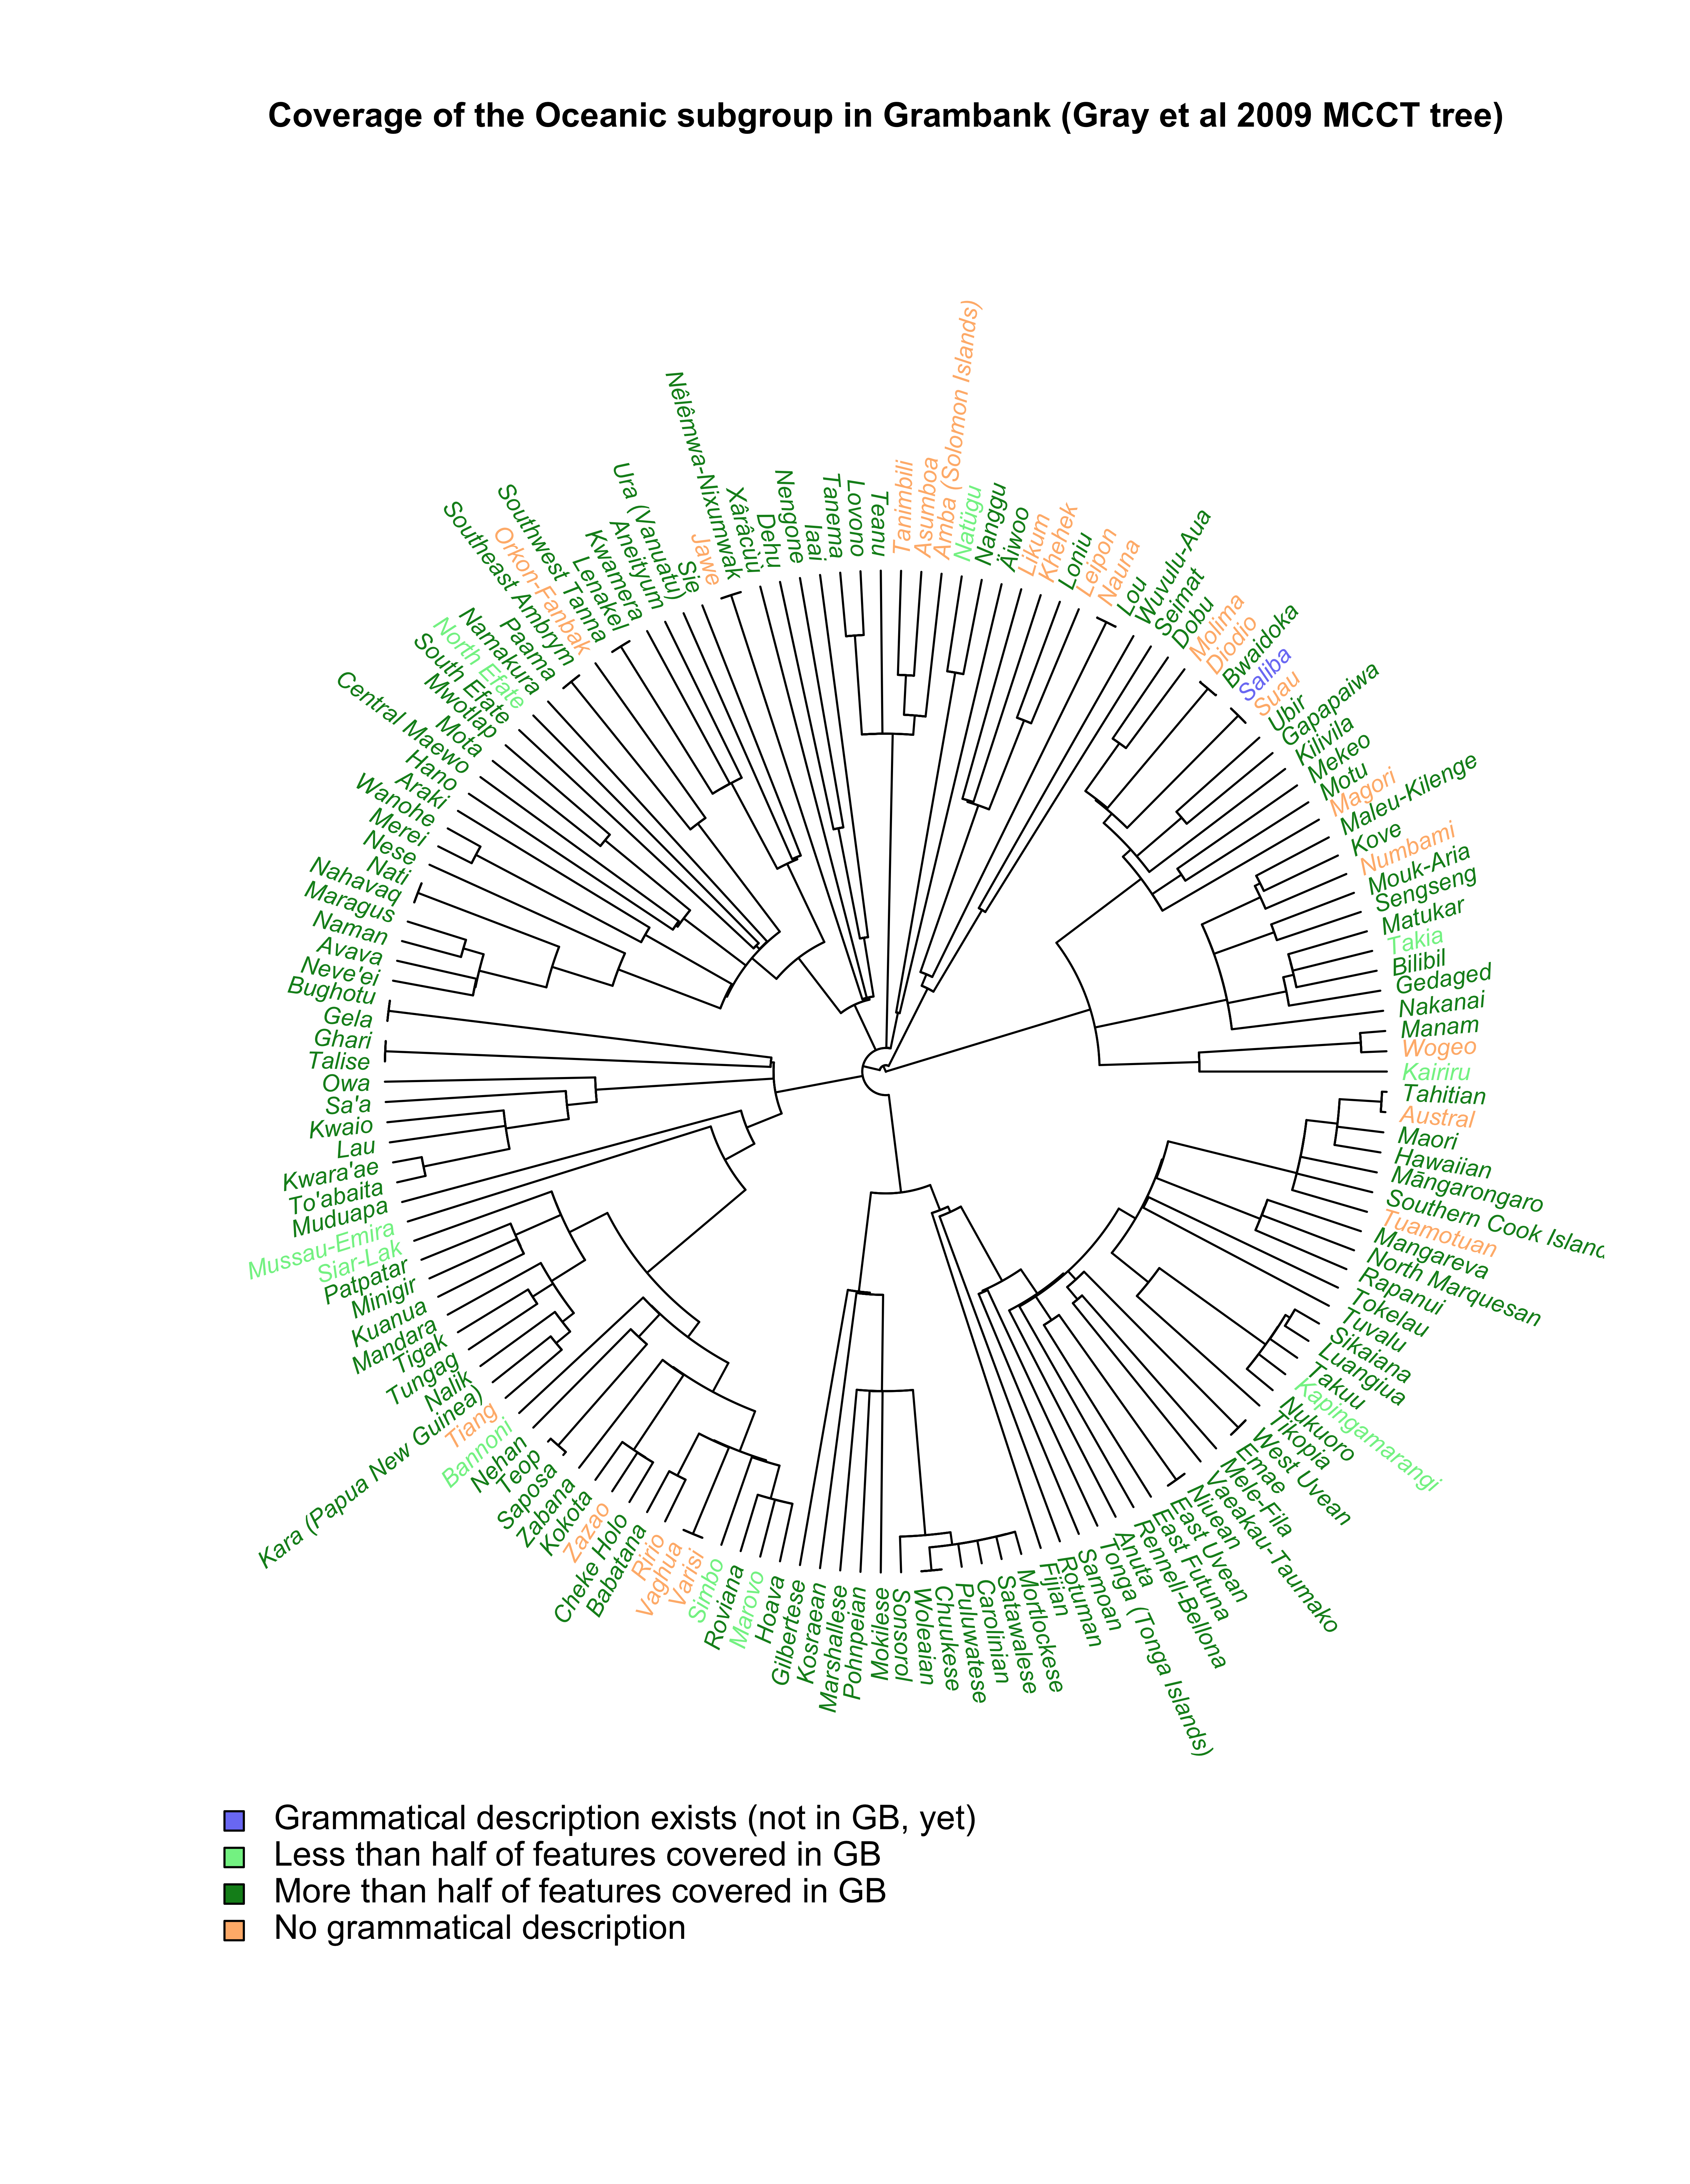
\includegraphics[width=\textwidth]{../code/output/coverage_plots/tree/Oceanic_tree_desc_status_gray_et_al_tree_mcct.png}
\caption{{Maximum Clade Credibility Tree of Oceanic from \citet{grayetal_2009}, with languages coloured for coverage in Grambank.}}
\label{tree_coverage_oceanic_gray}
\end{figure}

\begin{figure}[H]
\centering
\includegraphics[width=\textwidth]{../code/output/coverage_plots/tree/Oceanic_tree_desc_status_glottolog_tree.png}
\caption{\textbf{Tree of Oceanic from Glottolog, with languages coloured for coverage in Grambank.}}
\label{tree_coverage_oceanic_glottolog}
\end{figure}

One of the major differences between the trees is that the Glottolog-tree does not contain any information about branch lengths. All the branches in the Glottolog-tree are of the same length (1), whereas the branches in the Gray et al 2009-trees (the MCCT and the posteriors) have meaningful branch lengths based on rates of change in the underlying data (basic vocabulary) and calibration points (archaeological dates). This can be seen in the visualisations in Figures ~\ref{tree_coverage_oceanic_gray} and \ref{tree_coverage_oceanic_gray} where the first has varying lengths of branches but the latter all have a uniform length. This has the consequence that some tips in the Glottolog-tree are much further from the root than others. Further technical details of the trees can be found in Supplementary Material ~\ref{supp:tree_details}.

The Glottolog-tree contains, per definition, all the languages in the Oceanic subgroup in the Glottolog-dataset. Therefore the coverage per island group that is summarised in table ~\ref{GB_coverage_table_island_group} in the previous section applies to the Glottolog-tree as well. However, the \cite{grayetal_2009}-trees do not contain all Oceanic languages, but rather 155. Out of these 128 also occur in the Grambank dataset. A breakdown of coverage for the\cite{grayetal_2009}-trees per island group is found in table ~\ref{GB_coverage_table_island_group_gray}.

\begin{table}[h]
\caption{{Table showing coverage of Oceanic languages in Grambank per island group with matches to the Gray et al 2009-tree}}
\label{GB_coverage_table_island_group_gray}
\centering
\begin{tabular}{|l| p{2.7cm}| p{2.7cm} | p{2.7cm} |p{2.7cm} |}
  \hline
\textbf{Island group} & \textbf{\cellcolor{hedvig_orange!50}{No grammar}}  & \textbf{\cellcolor{hedvig_blue!50}{Grammar exists, but language not in Grambank (yet)}} &\textbf{\cellcolor{hedvig_lightgreen!50}{Less than half of the features covered in Grambank}} & \textbf{\cellcolor{hedvig_darkgreen!50}{More than half of the features covered in Grambank} } \\ 
  \hline
  Central Pacific & 2 & 0 & 1 & 28 \\ 
  Central Vanuatu & 1 & 0 & 1 & 16 \\ 
  Interior New Guinea & 0 & 0 & 0 & 0 \\ 
  Micronesia & 0 & 0 & 0 & 12 \\ 
  N Coast New Guinea & 6 & 2 & 2 & 3 \\ 
  New Caledonia & 1 & 0 & 0 & 5 \\ 
  Northern Vanuatu & 0 & 0 & 0 & 2 \\ 
  S New Guinea & 5 & 3 & 0 & 5 \\ 
  Solomons and Bougainville & 4 & 0 & 3 & 17 \\ 
  Southern Vanuatu & 0 & 0 & 0 & 6 \\ 
  Temotu & 3 & 0 & 1 & 5 \\ 
  Total & 22 & 5 & 10 & 118 \\ 
\end{tabular}
\end{table}

Finally, we are also using a sample of the posterior trees from \cite{grayetal_2009}. Their study yielded 4,200 posterior trees. Tree topologies that are more probable occur more often, but less probable trees also appear in the posterior. By using a set of possible trees instead of just one we can include other possible histories into our analysis, which could for example estimate contact events as well as inheritance. Figure ~\ref{densitree_plot} shows a visualisation of a 100 of the 4,200 trees which are used in this study.

\begin{figure}[H]
\centering
\includegraphics[width=\textwidth]{illustrations/gray_et_al_2009_100_sample_densitree.png}
\caption{\textbf{DensiTree \citep{bouckaert2014densitree} visualisation of the 100 random sampled trees from the Gray et al 2009-posterior.}}
\label{densitree_plot}
\end{figure}





\subsubsection{Data from historical linguistics on Oceanic proto-language grammar}
\label{sec:POC_lit_review}

The proto-languages of the Oceanic subbranch of the Austronesian language family are generally well researched in terms of their lexicon and phonology (see the book series on the Proto-Oceanic lexicon \citep{protooceanicvol1, protooceanicvol2, protooceanicvol3, protooceanicvol4, protooceanicvol5}, among other publications). There is also substantial work done on the grammar of Proto-Oceanic using the comparative method in historical linguistics. In this chapter I have summarised several major works in the field and distilled their research into testable hypotheses given the Grambank data and our methods. This section gives an overview of the works included and examples of how they have been incorporated into the study. Table~\ref{HL_prediction_table_summary} lists the publications used for the reconstruction of proto-Oceanic by historical linguists in this dissertation. 

13



For each of these publications, findings have been extracted that support a certain state of a Grambank feature at a certain node. For example, \citet[4]{marck2000_encyclo} writes that a causative prefix has been reconstructed for Proto-Polynesian (\emph{*faka-}). In the Grambank questionnaire we have the feature GB155 `\emph{Are causatives formed by affixes or clitics on verbs?}'. For the ancestral node that connects all the Polynesian languages, we should expect that for GB155 the state is either wholly or overwhelmingly ``1'' (yes/presence). For simplicity, I have only considered four ancestral languages: Proto-Oceanic, Proto-Central Pacific, Proto-Polynesian and Proto-Eastern Polynesian. The choice to focus on these four in particular was based on the fact that they are the most well-researched proto-languages in the literature. 

%For example,  (an ancestral language of Rotuman and Fijian separately from  Polynesian, Samoan and Northern Outliers excluding Eastern Polynesian). 


The literature suggests that Proto-Oceanic was a language with a pre-nominal definite/specific article \citep[136]{crowley1985common}, a distinction between inclusive and exclusive first person pronouns (\citet[112]{pawley1973some}, \citet[184]{crowley1985common}, \citet[500]{ross2004morphosyntactic}, \citet[67, 75]{lynchrosscrowley_proto_grammar_oceanic}), no gender distinctions in pronouns \citep[498]{ross2004morphosyntactic}, a dual number category in pronouns (\citet[498]{ross2004morphosyntactic}, \citet[69]{lynchrosscrowley_proto_grammar_oceanic} and \citet[173]{pawley1973some}), a distinction between alienable and inalienable possession\footnote{A distinction can be made between three different kinds of possessive classification: alienable/inalienable, direct/indirect and dominant/inactive. For the purposes of Grambank and this study, these are treated as similar enough to be included into the same category.} \citep[69]{lynchrosscrowley_proto_grammar_oceanic}, prepositions (\citet[167]{pawley1973some}, \citet[498]{ross2004morphosyntactic}), subject proclitics and object enclitics on the verb (\citet[498-499]{ross2004morphosyntactic}, \citet[83]{lynchrosscrowley_proto_grammar_oceanic}), possessive suffixes on the possessed noun (\citet[495]{ross2004morphosyntactic}, \citet[155]{pawley1973some}) and a transitivising suffix on verbs (\citet[352]{pawley1970change}, \citet[171]{pawley1973some}, \citet[80, 92]{lynchrosscrowley_proto_grammar_oceanic}). More reconstructions have been made, the full table is found in the appendix \ref{asr_table_appendic}. The reconstructions regarding ergativity will be presented separately.

Most of the time, the scholars of Proto-Oceanic are in agreement in their predictions. For example, \citet[142]{pawley1973some}, \citet[292]{ross2007two}, \citet[xiii, 125]{clark1976aspects} and \citet[89]{lynchrosscrowley_proto_grammar_oceanic} all propose that the proto-language of the Polynesian subgroup had a construction marking prohibitive that was different from declarative negatives. However, in some instances there are disagreements. As discussed earlier, one such case is the alignment system of Proto-Polynesian. \citet{clark1976aspects} claims that the system was ergative while \citet{hale_1968}, \citet{hohepa_1967,hohepa_1969} and \citet{chung1978} argue that Proto-Polynesian was accusative and several of the daughter languages developed ergativity later. Crucial to this arugment is also the nature and development of passive voice in Polynesian languages. Because of this disagreement, the results for the computational ancestral reconstruction for Grambank features regarding passive voice and ergativity will be presented separately from the others. There are 109 features in the larger set of non-controversial findings, and 11 in the subset that concerns passives and ergativity\footnote{Some of these are duplicates for different proto-languages, i.e. passive voice is examined for proto-Eastern Polynesian and for proto-Polynesian.}.

In the Grambank project, research assistants read published grammatical descriptions and extract information such that it fits with the definitions of our typological questionnaire (see section \ref{grambank}). This survey of the literature on Proto-Oceanic grammar is essentially the same task. Just as with the literature on reconstructed languages, scholars sometimes disagree on the nature of contemporary languages and how they should best be analysed. It is up to the coder, in this instance me, to make calls on which analysis to employ, what can be inferred from the literature and what should be left as unknown. It is possible to squeeze even more findings out of these publications; I have tended to be conservative in my interpretations. Out of the 201 (binarised) features in our questionnaire, 31\% (63) were answerable for Proto-Oceanic given this material. The average completion per language in the whole of the dataset is 72\%. 



\newpage
\section{Results}

\subsection{Concordance between traditional historical linguistics and computational methods}
In this study we are using the MCCT tree from \citet{grayetal_2009} and two models (Parsimony and Maximum Likelihood Estimation), making for two sets of results. Trees with more than half of the possible tips missing are discarded. The match between languages in Grambank and the Gray et al-tree is 112, meaning that results with less than 56 tips are ignored.  %#update

All results have been calculated in \texttt{R} \citep{R} using the packages \texttt{castor} (Parsimony) \citep{louca2017efficient}, \texttt{phangorn} \citet{phangorn}, \texttt{adephylo} \citep{jombart2017package}, \texttt{corHMM} \citep{corHMM}, \texttt{ape} \cite{paradis2004ape} and phytools \citep{revell2012phytools} and tidyverse \citep{tidyverse13}.


The full table of all predictions (excluding those relating to ergativity) and all results per feature, tree and method can be found in table~\ref{asr_table_appendic} in appendix \ref{ASR_comparison_table}. The summary results for the concordance with reconstructions by experts from historical linguistics are presented in table \ref{reconstruction_summary_table}. 
 
\begin{table}[H]
\centering
\caption{Comparison of how often the computational ancestral state reconstruction agrees with reconstruction from historical linguistics literature.}
\label{reconstruction_summary_table}
\begin{tabular}{|p{5cm}| p{2cm}|  p{2cm}| p{2cm} | p{2cm} |}
\hline
& \multicolumn{2}{c|}{Gray et al (2009)-tree}\\ \cline{2-3}
& \textbf{Parsimony} & \textbf{Maximum Likelihood} \\ \hline

 \cellcolor{hedvig_lightgreen!50}{Agree} & 95 & 91 \\ \hline
\cellcolor{hedvig_red!50}{Disagree} &13&10\\ \hline
 \cellcolor{hedvig_yellow!50}{Half / Half} &7&13\\ \hline

 \textbf{Accuracy score (incl Half/Half)} &0.857& 0.855 \\ \hline
 \textbf{Accuracy score (excl Half/Half)} &0.88&0.901\\ \hline
\cellcolor{hedvig_red!50}{False Negatives} &8 &8  \\ \hline
 \cellcolor{hedvig_lightgreen!50}{True Negatives} &42 &41\\ \hline
\cellcolor{hedvig_red!50}{False Positives} &5&2\\ \hline
 \cellcolor{hedvig_lightgreen!50}{True Positives} &53&50\\ \hline
\textbf{F1-score} & \textbf{0.891} & \textbf{0.909} \\ \hline


\end{tabular}
\end{table}

One of the most striking features of these results is the number of Half/Half predictions in the ML results. The ML approach takes into account the overall likelihood of the entire data, and for our dataset and trees this leads to more Half/Half results compared to the parsimony approach. One way of interpreting this is that the ML is more careful, it makes fewer confident predictions (more than 60\% either way), but it also disagrees less often with the findings from historical linguistics.

As was discussed earlier, there are several different ways of evaluating the performance of these approaches. If we consider how often they made a prediction that agreed with historical linguistics out of all the times they made a confident prediction (Accuracy score excl Half/Half), then ML. If we award half a point for Half/Half predictions, Parsimony does better. However, in both instances the numbers are very close to each other.

%We are comparing our computational reconstruction results to those predicted by expert linguists. The reason that the Glottolog tree is more in line with the predictions from historical linguistics is probably because it resembles the tree most historical linguists are used to more than the Gray et al-2009 tree does (the Glottolog tree is based on \citet{blust_2009,blust_2014} and \citet{blust_chen_2017}). That is not to say it is necessarily a better reflection of the true history of these languages, but rather that it may fit better with the underlying model that the field of historical linguistics has been working with in recent decades. Most of the literature on reconstructions of Proto-Oceanic does not include detailed accounts of the exact tree topologies and branch lengths used to reconstruct the ancestral languages. As was shown in section \ref{sec:asr_methods}, we had to impute branch lengths for the Glottolog-tree. The manner by which reconstructions are postulated in historical linguistics is typically by considering how well distributed the phenomena are over certain genealogical and areal subgroups. If the distribution is convincingly non-random and the comparative method can be used to reconstruct forms, predictions about the proto-language are made (c.f. \citet[109-110]{pawley1973some}).

%Furthermore, there were fewer matches between languages for which there is Grambank data and the Gray et al Tree, making for more uncertainty in predicting ancestral states.

In a similar study, \citet{jager2018using} attempt to reconstruct cognate classes for the proto-languages of three different language families. They used various approaches: binarising versus not binarising data; Maximum Parsimony versus Maximum Likelihood Estimation versus Minimal Lateral Networks; and using a single consensus tree versus sampling several from the tree posterior. The highest F1-score they achieved in this paper was 0.79 for the Maxmimum Likelihood Estimation reconstruction of Austronesian (using either a single tree or a sample of trees). This means that all of our results above perform ``better''. While this may be pleasing, it is not yet entirely clear why this is. 

In this study, only statements about ancestral languages that could be mapped to Grambank-features were included. It is  possible that the \citet{jager2018using} study had a greater overlap between all the reconstructions made by historical linguists and the meanings that they had data for. It is also possible that the set of features that were possible to include were also somehow easier to reconstruct, and if so that would explain the higher F1-scores.
%\label{sec:ars:metod:hist}

Many of the features that have been reconstructed for proto-languages of the Oceanic subgroup are also very common among Oceanic languages. For example, in our dataset 223 languages have a distinction between alienable and inalienable possession, and three do not have this feature . It is perhaps no surprise that historical linguists, Maximum Parsimony and Maximum Likelihood  agree that it is likely that the proto-languages have this feature as well\footnote{There was one exception. Maximum Likelihood on the Glottolog tree did not confidently predict presence of alienablity possession for Proto-Oceanic, the result was classified as ``half''. It did however predict alienablity for Proto-Polynesian.}. However, it is not always so simple. If this was all there was to it, we could just use raw distributions to reconstruct features of proto-languages. Historical linguists stress the importance of Maximum Parsimony and plausibility in their reconstructions, and as we saw in Fig. \ref{fig:clark_tree} (section \ref{sec:ars:metod:hist}), raw distributions alone can be misleading --- it is essential to take into account the tree structure. For example, \citet[118]{pawley1973some} suggests that verb-final word orders may have been possible in proto-Oceanic. This is tracked by feature GB133 \emph{`Is a pragmatically unmarked constituent order verb-final for transitive clauses?'}, and most languages are marked as `no' for this feature. However, Maximum Likelihood and the Gray et al 2009-tree did reconstruct presence of this feature at the root. 108 of the tips of this tree were absent, and 7 present, and yet the result was presence for Proto-Oceanic. This is (partially) due to the particular tree structure, where the languages with this feature attach further up in the tree structure (see Fig. \ref{GB133_tree_ML_gray})\footnote{It should be noted that the Maximum Parsimony result for the same tree did not reconstruct presence at the root. This has to do with the way Maximum Likelihood takes into account the distribution across the tree in each reconstruction, which gives the ancestral node of Maleu-Kilenge [male1289] and Kove [kove1237] a higher change of presence than it would under Maximum Parsimony.}\textsuperscript{,}\footnote{The languages with a presence for this feature are also mostly on the island of New Guinea and it is possible that this is a result of contact with non-Austronesian languages, as anonymous examiner 3 kindly pointed out.}.

\newpage
\begin{figure}
\centering
%\includegraphics[width=\textwidth]{illustrations/plots_from_R/ML_gray_-GB133.png}
\caption[Ancestral state reconstruction on tree for feature GB133, Gray et al 2009-tree and Maximum Likelihood.]{\textbf{Ancestral state reconstruction on tree for feature GB133, Gray et al 2009-tree and Maximum Likelihood. Yellow = presence, purple = absence.)}}
\label{GB133_tree_ML_gray}
\end{figure}


%
%It is often as revealing to study where the results got it ``wrong'' as where it was ``right''.Table~\ref{ASR_comparison_worst_table} shows the results for the automatic reconstructions that agreed the least with findings from classical historical linguistics. 
%
%%The two parsimony sets of results did propose that Proto-Oceanic did not have tense marking bound to the verb (GB082-GB084), nor is it by an inflecting word (GB121). However, when it came to tense marking by a particle and the aspect and mood marking, the automatic reconstructions were among the most dis-concordant with the expert predictions out of the entire dataset. In the Grambank dataset, we make a distinction between TAM-markers bound to the verb and free-standing markers that inflect versus those that don't. One possible factor that could have contributed to this is that TAM-markers in Oceanic languages are often described as forming portmanteau markers with subject markers. However, there is variation in how authors of grammars express this in their publications, and possibly also how our coders interpret the situation. This requires further investigation, which is unfortunately outside the scope of this study.

Besides the predictions made by historical linguists, we can also explore what else has strong support in our computational reconstructions that is not explicitly mentioned in the literature. For example, for Proto-Oceanic, three out of the four sets of results predicted that the order of numeral and noun is N-Num, all tests supported that ``adjectives'' in Proto-Central Pacific behaved like verbs when used predicatively, and all tests also supported that Proto-Polynesian had three or more distance contrasts among demonstratives. 

\subsection{Where the conflicts are: Ergativity}
The nature of the alignment system of Proto-Polynesian is contested, and therefore the features that concern passive voice and ergativity are presented separately from the rest. \citet{clark1976aspects} posits, primarily on the basis of parsimony, that Proto-Polynesian was ergative whereas \citet{hale_1968}, \citet{hohepa_1967,hohepa_1969}, and \citet{chung1978} argue that it was accusative (while they suggest different historical pathways, they agree that Proto-Polynesian was nominative-accusative).

Grambank has two features that pertain to this argument:

\begin{itemize}
\item GB408 \emph{Is there any accusative alignment of flagging?}
\item GB409 \emph{Is there any ergative alignment of flagging?}
\end{itemize}

It is entirely possible for a language to be entered into the database as ``yes'' for several of these, i.e., from the perspective of Grambank languages aren't ``ergative'' or ``accusative'' --- they can have both ergative and accusative flagging simultaneously. This makes it possible for us to prove both Chung and Clark ``right'', the results can come out such that Proto-Polynesian had both accusative \emph{and} ergative alignment flagging. However, the results do come out strongly in favour of the proposal by Clark. Table \ref{proto_poly_erg_table} shows that both methods reconstruct ergative alignment for Proto-Polynesian, and only one method predicts a half/half chance of a nominative/accusative system. This lends support to Clark's suggestion that Proto-Polynesian was ergative.

\begin{table}[H]
\centering
\caption{Table showing the results for the alignment system of Proto-Polynesian}
\label{proto_poly_erg_table}
\begin{tabular}{|l|l|l|l|l|l|l|l|}
\hline
Feature & \textbf{Parsimony}& \textbf{Max Likelihood} \\ \hline
GB408 \emph{Is there any accusative alignment of flagging?} &Absent & half \\
GB409 \emph{Is there any ergative alignment of flagging?} & Present & Present \\
\end{tabular}
\end{table}


% latex table generated in R 4.1.0 by xtable 1.8-4 package
% Thu Oct 14 12:48:01 2021
\begin{table}[ht]
\caption{Table showing the results for the conflcts}
\label{conflict_table}
\centering
\begin{tabular}{rllrllllllll}
  \hline
 & Feature\_ID & Proto-language & Prediction & Source & Parsimony result (Glottolog-tree) & Parsimony result (Gray et al 2009-tree) mcct & Parsimony result (Gray et al 2009-tree) posteriors & ML result (Glottolog-tree) & ML result (Gray et al 2009-tree) mcct & ML result (Gray et al 2009-tree) posteriors & result\_most\_common \\ 
  \hline
1 & GB408 & Proto-Polynesian & 1.00 & Chung (1978:261-262), Ball (2007) & False Negative & False Negative & False Negative & False Negative & False Negative & Half & False Negative \\ 
  2 & GB408 & Proto-Polynesian & 0.00 & Clark (1976:106-107) & True Negative & True Negative & True Negative & True Negative & True Negative & Half & True Negative \\ 
  3 & GB409 & Proto-Polynesian & 0.00 & Chung (1978:261-262) & False Positive & False Positive & False Positive & False Positive & False Positive & False Positive & True Negative \\ 
  4 & GB409 & Proto-Polynesian & 1.00 & Clark (1976:106-107) & True Positive & True Positive & True Positive & True Positive & True Positive & True Positive & False Negative \\ 
  5 & GB409 & Proto-Central Pacific & 1.00 & Kikusawa (2002:1) & False Negative & False Negative & False Negative & False Negative & False Negative & False Negative & False Negative \\ 
  6 & GB409 & Proto-Central Pacific & 0.00 & Ball (2007) & True Negative & True Negative & True Negative & True Negative & True Negative & True Negative & True Negative \\ 
   \hline
\end{tabular}
\end{table}


As was noted earlier, the computational reconstructions differ from those arrived at through the comparative method primarily because the data used in this study is abstract presences or absences of structural features whereas historical linguists use specific concrete forms instead (c.f. \citet{crowley1985common}). In the case of alignment systems, the matter of concrete markers is less of an issue. However, besides the parsimony principle (as laid out by \citet[19]{clark1976aspects} for example), expert historical linguists also take into account the plausibility of the proposed proto-language and the chain of changes posited \citep{chung1977aspects}. It is not possible for the computational reconstructions to take these assumptions into account without having them formally described and introduced into the model, which is not possible at this time. This may be the reason for the lack of support for Chung's theory; the crucial information that underpins it is not accounted for in this study.

Given the topology of the two trees used in this study, where the ergative flagging language Tongan is always attached to the Proto-Polynesian root at a higher level than Eastern Polynesian languages, it is very likely that GB409 would be reconstructed as present for Proto-Polynesian. As Clark pointed out, it is the most parsimonious solution. However, it could still have been the case that GB408 (accusative) or GB410 (neutral alignment) would have been reconstructed for Proto-Polynesian. The reasons for this may lie in different definitions of what counts as nominative-accusative or neutral in different descriptions, and/or in discussions of plausibility. As has been discussed earlier, it was not possible to include plausibility as a factor in this study.

The proposals of \citet{hale_1968}, \citet{hohepa_1967, hohepa_1969}, and \citet{chung1978} also involve reconstruction of passive voice that relate to the development of the ergative systems. They suggest different pathways by which languages can develop from a nominative-accusative system to an ergative-absolutive one that rely on changes in the specifics of the passive voice construction that we unfortunately do not track. Given our data, which simply records presence of a productive passive voice marker on the verb, we are not able to scrutinise the three precise theories in greater detail. The results largely support the hypothesis that Proto-Eastern Polynesian had a passive voice marker and that Proto-Oceanic and Proto-Polynesian did not. %This can be seen as partial support for the proposals by \citet{hale_1968, hohepa_1967, hohepa_1969, chung1978}.


%###############


%
%\subsubsection{Stability of features}
%\label{sec:asr:stability}
%
%We assess the stability of the features in our data by measuring the Parsimony cost (number of changes in the tree) and the rate of gains and losses in the ML results. Features where more than half of the languages of the tree were missing were excluded from these results.
%
%Parsimony cost represents the number of changes inferred as part of the most parsimonious solution. Trees where all the tips are of the same value will have a parsimony cost of 0, since no change occurred. A parsimony cost of 1 will indicate that 1 change occurred somewhere in the tree, and so on.
%
%The ML results produce a rate of gain and loss for each feature given the full tree. In order to make the rates comparable across features, all the trees used have the same number of tips (with tips with missing data being converted to ambiguous states). For the results, the average rate (mean of rate of gain and loss) is considered.
%
%The large majority of the most stable features are dominated by rare phenomena. For example, all four sets of results rank the following two features as among the five most stable:
%
%\begin{enumerate}
%    \item GB110 \emph{Is there verb suppletion for tense or aspect?}
%    \item GB149 \emph{Is there a morphologically marked inverse on verbs?}
%\end{enumerate}
%
%However, these are both entirely absent from the entire group. There is no Oceanic language in Grambank with verb suppletion for tense or aspect, nor a language with inverse marked on verbs. It is little wonder that these features are stable, no change is needed from the reconstructed root (absence) to all the tips (also absence). This is a characteristic of some of the results from the study by \cite{dediu2013some} as well: many of the most stable features in their overview were also rare.
%
%In order to avoid the most rare features, the results are also reported for only features where the balance of presence/absence is at least 5\% one way and 95\% the other. The top and bottom five for each method and tree are reported in appendix \ref{stability_tables}, including a separate table for stable features with at least a distribution of 5\%/95\%.
%
%Table \ref{summary_stability} is a summary of the top-5 most stable features in each of the four sets of results, including only features with a distribution of at least 5\%/95\%.
%
%\begin{table}
%\centering
%\caption{Top 5 most stable features per method and tree, only including features with a distribution of at least 5\%/95\%.}
%\label{summary_stability}
%\begin{tabular}{?l?p{2cm}?p{2cm}?p{2cm}?p{2cm}?l?l?l?l}
%\hline
%\multirow{2}{*}{\textbf{Grambank Feature}}& \multicolumn{2}{c|}{\textbf{Glottolog 4.0-tree}}& \multicolumn{2}{c|}{\textbf{Gray et al (2009)-tree}}\\ \cline{2-5}
%& \textbf{Parsimony} & \textbf{Maximum Likelihood} & \textbf{Parsimony} & \textbf{Maximum Likelihood} \\ \hline
%\textbf{GB081 VInfix}& {} & \cellcolor{hedvig_lightgreen!50}{Top-5} & \cellcolor{hedvig_lightgreen!50}{Top-5} & \cellcolor{hedvig_lightgreen!50}{Top-5} \\ \hline
%\textbf{GB433 POSSSfxPosd}& {} & \cellcolor{hedvig_lightgreen!50}{Top-5}& {} & {} \\ \hline
%\textbf{GB131 TransVInitOrder}& {} & \cellcolor{hedvig_lightgreen!50}{Top-5}& {} & {} \\ \hline
%\textbf{GB132 TransVMedOrder}& {} & \cellcolor{hedvig_lightgreen!50}{Top-5}& {} & {} \\ \hline
%\textbf{GB024b OrderNNUM}& {} & \cellcolor{hedvig_lightgreen!50}{Top-5}& {} & {} \\ \hline
%\textbf{GB188 AUGBound} & \cellcolor{hedvig_lightgreen!50}{Top-5}& {} & \cellcolor{hedvig_lightgreen!50}{Top-5}& {} \\ \hline
%\textbf{GB422 ComplThinkKnowPost} & \cellcolor{hedvig_lightgreen!50}{Top-5}& {} & \cellcolor{hedvig_lightgreen!50}{Top-5}& {} \\ \hline
%\textbf{GB300 VSupplGive}& {}& {} & \cellcolor{hedvig_lightgreen!50}{Top-5}& {} \\ \hline
%\textbf{GB095 CaseSplitTAM}& {}& {} & \cellcolor{hedvig_lightgreen!50}{Top-5}& {} \\ \hline
%\textbf{GB133 TransVFinalOrder} & \cellcolor{hedvig_lightgreen!50}{Top-5}& {} & {} & {} \\ \hline
%\textbf{GB264 QPartMedial} & \cellcolor{hedvig_lightgreen!50}{Top-5}& {} & {} & {} \\ \hline
%\textbf{GB330 RELCorr} & \cellcolor{hedvig_lightgreen!50}{Top-5}& {} & {} & {} \\ \hline
%\textbf{GB091 A-ArgSfxV}& {} & {} & {} & \cellcolor{hedvig_lightgreen!50}{Top-5} \\ \hline
%\textbf{GB333 NUMDecimal}& {} & {} & {} & \cellcolor{hedvig_lightgreen!50}{Top-5} \\ \hline
%\textbf{GB148 AntipassiveBoundV}& {} & {} & {} & \cellcolor{hedvig_lightgreen!50}{Top-5} \\ \hline
%\textbf{GB335 NUMVigesimal}& {} & {} & {} & \cellcolor{hedvig_lightgreen!50}{Top-5} \\ \hline
%
%\end{tabular}
%\end{table}
%
%These results indicate that there is little agreement between the methods as to which features are most stable. Three out of four sets of results rank verbal infixing (GB081) as among the five most stable and while it is indeed less rare than 5\%/95\%, it is not much rarer. Only 8\% of the languages in the sample have this feature.
%
%There are a few interesting features in this summary table. Counting systems (GB333 and GB335) are often said to be stable. There are also a few word-order related features, which is in line with previous research \citep[c.f.][]{dediu2013some}.
%
%However, overall these results do not strongly support that certain features are more stable than others consistently. This is likely because Oceanic is not a deep enough genealogical unit for this kind of analysis. Features are either overwhelmingly present or absent with little in between. This makes phylogenetic analysis difficult. It is possible to consider other factors besides time-depth as relevant factors for stability, such as social network structure/political complexity (see section \ref{prediting:sec:pol:complex}), but this is outside the scope of this study. Furthermore, it is possible that the characteristics of structural data are such that it is much more difficult to apply ancestral reconstruction methods
%(there are several different reasons for the presence of a structural feature, and they may be unrelated, see \ref{subsection:comp_lex_str} and section \ref{sec:ars:metod:hist}).
%
%
%
%
%\subsubsection{Conservatism per language}
%\label{sec:conservatism}
%Conservatism is a measurement of how much change there has been from the reconstructed root of the tree (proto-Oceanic) down to each of the tips (languages). A high number indicates a large amount of change has occurred between the root and the tips. The change can go back and forth, i.e. flip between presence and absence of a feature several times between the root and the tip.
%
%This is different from the direct pairwise dissimilarity between each language and a reconstructed version of Proto-Oceanic which we saw in section \ref{aberr_dist_results}. The analysis of pairwise dissimilarity did not take into account the intermediate nodes between Proto-Oceanic and each language, and only included the features where findings in historical linguistics indicated a particular feature in Grambank for Proto-Oceanic. The analysis here differs in two important ways: a) the state of the intermediate nodes are taken into account and b) the tips are compared to the computationally reconstructed Proto-Oceanic (which includes more features than there are findings for in historical linguistics).
%
%For the two parsimony sets of results, conservatism was calculated by a kind of parsimony analysis known as ACCTRAN (ACCelerated TRANsformation). This lets us examine how many changes occur from the root down to each of the tips according to the most parsimonious solution of ancestral states. 
%
%For the ML analysis, the function \texttt{optim.ml()} was used to rescale the branches in accordance with the changes that the ML (marginal) reconstruction posited. The result of \texttt{optim.ml()} is an unrooted tree, which is why it is necessary to reroot. Nanggu [nang1262] was used as an outgroup to root the trees, since it is well-known as an Oceanic outlier.
%
%In order to make the results comparable across the two methods, the ACCTRAN trees were also re-rooted with Nanggu as an outgroup. Because Nanggu was used as an outgroup, features which Nanggu lacked were excluded. This left 167 Grambank features which were included in the conservatism analysis. 
%
%The results from both the Maximum Parsimony and Maximum Likelihood were rescaled to between 0 and 1 in order to make them comparable. A score of 1 means that a great deal of change has occurred, whereas a score of 0 means that no change has occurred. Fig. \ref{map_br_lens} shows the languages of the sample coloured by conservatism in each of the four sets of results given our two methods and two trees.
%
%%The language in Papua New Guinea that appears as a bright yellow (progressive) point in Papua New Guinea in the results based on Maximum Likelihood is Kilivila [kili1267]
%
%
%\newpage
%\begin{sidewaysfigure}
%\centering
%\includegraphics[width=\textwidth]{illustrations/plots_from_R/br_len_maps.png}
%\caption[Map of Oceanic languages and their average conservatism given the four sets of results.]{\textbf{Map of Oceanic languages and their average conservatism given the four sets of results. Yellow = progressive, blue = conservative. First row: Maximum Likelihood branch lengths, second row: Parsimony cost. First column: Glottolog-tree, second column: Gray et al 2009-tree.)}}
%\label{map_br_lens}
%\end{sidewaysfigure}
%
%Across the four sets of results the map visualisation indicates that the most conservative regions appear to be the Bismarck archipelago and Temotu (see Fig. \ref{Marck_map_with_language_names} in section \ref{subregion:sailing} for locations of Bismarck and Temotu).
%
%In order to evaluate the conservatism of the different regions in our data the languages were grouped into island groups. The same groups as in paper \ref{paper_distances} were used with the addition of three groups in Near Oceania, making for a total of ten groups (ordered by mean conservatism averaged over all four sets of findings): Temotu, Bismarck, Solomons and Bougainville, Northern Vanuatu, New Caledonia, New Guinea Mainland/Louisiade Archipelago, Micronesia, Central Vanuatu, Central Pacific and Southern Vanuatu. 
%
%Figs. \ref{ridgeplot_BR_len_MP} and \ref{ridgeplot_BR_len_ML} show the distribution of conservativeness across the island groups over the four methods. The ridgeplots represent the distribution of conservativeness in each island group but points have also been added to show the precise locations of the data-points. The line and label on each distribution indicates the mean. For the analysis with the Gray et al 2009-tree there were unfortunate only two languages of the Northern Vanuatu group present, which is not enough to generate a ridgeplot but the points indicate the values of the languages there.
% 
%%% latex table generated in R 4.0.0 by xtable 1.8-4 package
%%% Sun Apr 26 22:18:59 2020
%%\begin{table}[H]
%%\centering
%%\caption[Island groups ordered by mean conservatism.]{Island groups ordered by mean conservatism. A score of 1 means that a great deal of change has occurred, whereas a score of 0 means that no change has occurred.} 
%%\label{conservatism_group_parsimony_Gray}
%%\begin{tabular}{lr}
%%  \hline
%%Island group & Average distance from root\\ 
%%  \hline
%%Temotu & 0.18 \\ 
%%  Bismarck & 0.46 \\ 
%%  Solomons and Bougainville & 0.52 \\ 
%%  Northern Vanuatu & 0.52 \\ 
%%  New Caledonia & 0.54 \\ 
%%  New Guinea mainland / Louisiade archipelago & 0.56 \\ 
%%  Micronesia & 0.57 \\ 
%%  Central Vanuatu & 0.58 \\ 
%%  Central Pacific & 0.64 \\ 
%%  Southern Vanuatu & 0.68 \\ 
%%   \hline
%%\end{tabular}
%%\end{table}
%
%\begin{sidewaysfigure}
%\centering
%\includegraphics[width=\textwidth]{../code/output/other_plots/br_len_ridgeplots_gray.png}
%\caption{{Ridgeplots of the distribution of conservatism over the island groups per method.}}
%\label{ridgeplot_BR_len_MP}
%\end{sidewaysfigure}
%
%The results from the different methods and trees differ, we shall take a closer look at this later and compare the scores to each other and to time of settlement.
%
%Temotu is the most conservative group in the sample across all the four sets of findings. If we average the conservatism of all the analyses, Temotu languages have a mean of 0.18 conservatism compared to Bismarck's 0.46. However, Nanggu was used to outgroup root the tree, which makes Nanggu the first split from proto-Oceanic in the tree which was used in the reconstruction. This is likely to have inflated the conservatism of Nanggu and therefore the conservatism of its closest relatives, which are other languages in the Temotu group. This is likely to have enhanced the conservatism of the Temotu island group. However, it should be noted that Temotu languages did also have the lowest direct distance to Proto-Oceanic as reconstructed by historical linguists (section \ref{aberr_dist_results}).
%
%It is possible that if certain ancestral nodes in the tree had been anchored by archaeological accounts, such as those found in \cite{rieth_cochrane_2018} or \citet{kirch2017road}, Temotu would have been less likely to be the most conservative. This is because the settlement order would definitely be Bismarck first and Temotu later.
%
%Historical linguistics research indicates that the most likely homeland of Oceanic is found in the Bismarck archipelago \citep[97]{lynchrosscrowleyinternalsubgroupingoceanic}. The second most conservative group in our sample is indeed Bismarck, which supports this notion.
%
%As was discussed in the previous paper (\ref{paper_distances}) certain languages of Temotu, Southern Vanuatu and New Caledonia are known to be unusually innovative lexically and phonologically \citep{grace1981indirect, grace_1992_aberrant, pawley2006explaining}. In the previous paper, we saw that Temotu and New Caledonia were more unusual lexically than Southern Vanuatu, and that structurally there was little difference. In these results however,  Southern Vanuatu is the most progressive in the MP results, and in the mid-range in the ML-results, whereas Temotu is the least conservative overall and New Caledonia appears in the mid-range in all the results. It appears that it took more transitions back and forth to ``get to'' the structure of Southern Vanuatu languages compared to the other two ``aberrant'' groups Temotu and New Caledonia.
%
%The languages of the Central Pacific are known as especially \emph{conservative} in their lexicon (\citet{blust1981, blust2000lexicostatistics} and \citet{pawley_2009_solomons}). However, this seems to not hold structurally. The Central Pacific Languages are the most progressive in the MP results (after Southern Vanuatu) and in the upper-mid range in the ML results. A few features that make the Central Pacific languages stand out are the lack of subject markers as prefixes or proclitics on verbs (GB090 \& GB092) as well as the presence of ergative case marking (GB409) and passive voice (GB147).
%
%%##here is where you are
%
%However, there are a few methodological considerations that are important to the interpretation of these results, in particular concerning Central Pacific. The difference between the Maximum Parsimony and Maximum Likelihood results are most likely due to branch lengths and the number of nodes between each tip and the root. For the Maximum Parsimony analysis, the branch lengths are irrelevant. Maximum Parsimony only reconstructs states at each intermediate node, regardless of how close that node is to another. This means that if there are more nodes between the root and the tip, Maximum Parsimony has more ``opportunity'' to posit changes than if there were fewer. The Maximum Likelihood analysis however takes into account the length of the branches, which in turn means that the particular number of nodes between the root and the tips is of less importance.
%
%The two trees we have used in this analysis, the Glottolog tree\footnote{Note that both trees have been binarised for the analysis in this paper.} and the Gray et al 2009-trees, have a structure such that there are more nodes between the languages of Central Pacific and the root (Proto-Oceanic) than there are between languages of Central Vanuatu and the root. The tree topologies are displayed in section \ref{asr:sec:GBcoverage}, but as it is difficult to appreciate this difference in the plots there I have summarised the number of nodes between tips and root per island group in table \ref{table_mean_nodes}. The precise number of nodes between the tips and root differ between the two trees, and also between the two methods since the Parsimony analysis drops tips with missing data. However, the rank orders are largely the same, with Temotu languages having the fewest number of nodes between them and the root and Central Pacific the most.
%
%% latex table generated in R 4.0.0 by xtable 1.8-4 package
%% Fri May 29 13:23:48 2020
%\begin{table}[ht]
%\caption{Mean number of nodes between tips and root per method and tree.}
%\label{table_mean_nodes}
%\centering
%\begin{tabular}{?l?  p{2cm} ?p{1.5cm}p{1.5cm}p{1.5cm}p{1.5cm}?}
%  \hline
%  &   \multicolumn{5}{c?}{\textbf{Mean number of nodes between tips and root} } \\    \cline{2-6}
%& &  \multicolumn{2}{c|}{\textbf{Max Parsimony}} &\multicolumn{2}{c|}{\textbf{Max Likelihood}}\\ \cline{3-6}
%\textbf{Island group} & \textbf{All} &  \textbf{Glottolog }& \textbf{Gray} & \textbf{Glottolog} & \textbf{Gray}  \\ \hline
%
%%Island group & All & MP Glottolog & MP Gray et al 2009 & ML Glottolog & ML Gray et al 2009 \\ 
%  \hline
%Temotu & 2.95 & 2.83 & 2.58 & 3.25 & 3.14 \\ 
%  New Caledonia & 9.85 & 11.19 & 7.73 & 12.08 & 8.40 \\ 
%  Southern Vanuatu & 10.29 & 10.56 & 9.15 & 11.62 & 9.83 \\ 
%  New Guinea mainland / Louisiade archipelago & 10.66 & 11.67 & 8.35 & 12.31 & 10.33 \\ 
%  Micronesia & 11.32 & 11.92 & 10.08 & 12.37 & 10.92 \\ 
%  Northern Vanuatu & 11.51 & 11.94 & 10.31 & 13.80 & 10.00 \\ 
%  Bismarck & 11.77 & 13.18 & 9.24 & 13.24 & 11.43 \\ 
%  Central Vanuatu & 12.47 & 12.90 & 11.21 & 13.15 & 12.62 \\ 
%  Solomons and Bougainville & 12.96 & 14.45 & 9.91 & 15.58 & 11.88 \\ 
%  Central Pacific & 14.55 & 15.20 & 12.80 & 16.54 & 13.67 \\ 
%   \hline
%\end{tabular}
%
%\end{table}
%
%Since there are more nodes between Central Pacific and the root this means that the Maximum Parsimony algorithm has more ``chances'' to posit changes. This is not true of the Maximum Likelihood analysis which is able to posit changes in relation to the branch lengths and cares less about the precise number of nodes on the tree. Fig. \ref{BR_len_to_nnodes} shows the language conservatism score per method and tree compared to the number of nodes between the languages and the root. There is a stronger correlation between the number of nodes along the route from a specific language (tip) to the root and the Maximum Parsimony scores of conservatism for that language (upper row) than there is between the Maximum Likelihood and the number of nodes (lower row). The correlation between the number of nodes and the Maximum Likelihood, though significant, is very weak.
%
%\begin{figure}[H]
%\centering
%\includegraphics[width= \textwidth]{illustrations/plots_from_R/br_len_compare_to_nodes.png}
%\caption{Scatterplots comparing number of nodes from root to tips and conservatism scores.}
%\label{BR_len_to_nnodes}
%\end{figure}
%
%This means that the Maximum Parsimony conservatism score is mainly reproducing the number of splits between the language and the root --- the more splits, the higher the Parsimony cost (amount of change). Conversely, fewer splits mean less change (lower Parsimony cost). Temotu languages are more conservative in the Parsimony analysis than in the Maximum Likelihood analysis, and the outgroup-rooting with Nanggu results in fewer nodes between the root and the Temotu languages. Whether or not this is good or bad depends on what we think splits in the tree represent. Do we expect languages which are more deeply nested in a family tree to have had a more tumultuous history? Or do we think that the rate of change is not correlated with the number of splits found in the tree --- that ``early'' off-shoots like Nanggu and Yapese are equally likely to undergo substantial changes as Central Pacific language which have more splits in their lineage? 
%
%Furthermore, sub-nesting may also be a product of research efforts --- areas which have been more well-researched may be better represented in the tree of Glottolog than those which have had comparatively less research. Note that this is not as relevant for the Gray et al 2009-tree which is based on lexical and archaeological data, not compilations of historical linguists' accounts like the Glottolog tree\footnote{A total of 102 references are used in Glottolog for the structure of the Austronesian family tree, with the main references being \citet{blust_2009, blust_2014} and \citet{blust_chen_2017}.}. It is beyond the scope of this dissertation to reach any final conclusions on how we should interpret the nature of splits in these trees. The findings of this paper indicate that the more splits in a lineage the less conservative the language is in the Maximum Parsimony analysis, which informs us that the Maximum Parsimony is adding little information concerning conservatism beyond the number of splits. How we should interpret the number of splits is however not clear.
%
%Bringing this back to the specific island groups, it is still noteworthy that Central Pacific is not among the most conservative languages structurally in either of the four sets of results. This goes against what we might have expected given the lexical conservatism of these languages found in other publications. 
%
%More remarkable perhaps in light of the correlation between number of nodes and the Maximum Parsimony conservatism score is the progressiveness of Southern Vanuatu languages and the conservatism of Bismarck languages. Table \ref{table_mean_nodes} shows that Southern Vanuatu languages have the third least number of nodes on average between the root and the languages, and Bismark's languages appear in the mid range. And yet, the Southern Vanuatu languages are among the most progressive in the results, with Bismarck languages among the most conservative. This indicates that the progressiveness of the Southern Vanuatu languages and the conservatism of the Bismarck languages are robust findings.
%
%We can also compare the conservatism of the languages across the methods, and to known settlement dates. Fig. \ref{SPLOM_BR_len} shows a scatterplot matrix comparing the four conservatism-per-language scores to each other and also to settlement order (see section \ref{pol_complex_sec_dates} in paper \ref{paper_pol_complex}). The lower triangle shows scatterplots of different combinations of data. The cell in the second row and first column displays a scatterplot of the two ML results compared against each other. The dexter diagonal shows the histograms of the various datasets. The upper triangle shows the Pearson's statistic. Stars indicate significance in the conventional manner. 
%
%\begin{figure}[H]
%\centering
%\includegraphics[width=\textwidth]{illustrations/plots_from_R/br_len_splom_SFM.png}
%\caption{{Scatterplot matrix of correlations between conservatism scores over the four different sets of results, and settlement order.}}
%\label{SPLOM_BR_len}
%\end{figure}
%
%There is a very strong correlation between the two ML results (0.94), even though the two tree topologies are quite different. This is noticeable, we might expect that analysis using such different trees would generate more different results. The correlation between the two parsimony results is also strong (0.79), but not as strong. The parsimony results also correlate with the settlement time, the Glottolog and Maximum Parsimony results moderately (0.55) and the Gray et al 2009 and Maximum Parsimony weakly (0.35). This indicates that the higher the Parsimony cost (i.e. rate of change), the more likely a language is to be spoken on an island which has been settled more recently. This correlation, though present, is not strong and needs to be further investigated. It is possible that the correlation between the Maximum Parsimony conservatism scores and settlement time depth is related to the aforementioned relationships to degree of nesting (i.e. number of nodes between root and tip).
%
%The fact that the two Maximum Likelihood results correlate more with each other than the two Maximum Parsimony results does suggests that it is a more robust methodology.
%
%In summary, the results differ between the four methods, and these differences reveal some of the consequences behind the methodologies. Since Maximum Parsimony is more dependent on the number of nodes along a lineage, the findings show that it adds little information beyond that. The interpretation of the precise results depends on how we choose to interpret what it means that the lineages of certain languages involve more splitting events than others. Regardless, the findings indicate that Central Pacific languages are \emph{not} especially conservative structurally, that the Bismarck languages are indeed particularly conservative and that the ``aberrant'' island group of Southern Vanuatu appears especially innovative structurally. For future studies, it is possible to investigate the drivers behind conservatism in a similar manner to how language richness is explored in paper \ref{paper_pol_complex}.
%
%
%%The distribution of conservatism over these languages looks more similar to the settlement pattern, with more recently settled areas overall being more progressive. In paper \ref{paper_pol_complex}, we used archaeological dates for a model on factors of language diversification in the region (see Fig.\ref{dates_map} for a map of time of settlement). If we compare the time depth-data from that study to these Parsimony costs using a Pearson's product-moment correlation we do find a statistically significant positive correlation (cor = 0.59, \emph{p} value = 2.1 * 10 $^-13$). In the case of islands and atolls in Eastern Polynesia and the northern Polynesian outliers, their high rate of change could be due to bottleneck effects (c.f. \citet{bromham_polynesian_sizes}).
%
%%In summary, structural features of language may be subject to different pressures than lexical (c.f. \citet{francois2011}). These results indicate that the retention rate of structural features is different from that ofbasic lexicon.

\section{Conclusions}
In this paper, we have investigated the history of structural features of Oceanic languages to examine how computational reconstructive methods compare to reconstructions by historical linguists (including contributing to the debate on Proto-Polynesian alignment), the stability of features and conservatism of languages of the region.

We have found that computational reconstructions show a high degree of concordance with reconstructions from expert historical linguists. Reconstructions by both Maximum Parsimony and Maximum Likelihood agreed to a very large extent with the findings from historical linguistics, but Maximum Likelihood was most likely to be ``hesitant'' and posit half/half states.

Within Oceanic historical linguistics, there exists a debate regarding the nature of the alignment system of Proto-Polynesian. The results of this study support the analysis that it was ergative. However, since the computational reconstructions are unable to take into account considerations of plausibility, which is the main difference between the different proposals, this cannot be taken as hard evidence.

One of the aims of this study was also to explore stability of features. The results reaffirmed previous studies which have found rare features among the most stable \citep{dediu2013some}. We also expected features that pertain to paradigmatic distinctions to be more likely to be stable. However, this was not the case. The results from Maximum Parsimony and Maximum Likelihood were overall not in agreement.

More work is needed to explore the hypothesis that certain diagnostic structural features can track history at a deeper time depth than basic vocabulary \citep[c.f.][]{nichols1998origin}. The results of this study were inconclusive, possibly because Oceanic is not deep enough for this kind of analysis.

The last part of the study investigated rates of change over languages of the region. Languages of the Bismarck archipelago are the most conservative overall\footnote{Disregarding Temotu which most likely has a high conservatism score because  of the outgroup-rooting.}. The distribution of conservatism supports the theory that we are more likely to find conservative languages at the origin of the spread  \citep[119]{lynchrosscrowleyinternalsubgroupingoceanic}. Contrary to other findings in historical linguistics concerning lexical conservatism, languages of the Central Pacific were not the most conservative and potentially even among the most progressive. Southern Vanuatu languages were also found to be particularly progressive structurally.



\newpage


Linguistic diversity can mean many things. This dissertation has explored four different ways of conceiving of diversity: number of languages (paper \ref{paper_pol_complex}), pairwise dissimilarity between languages (paper \ref{paper_distances}), rate of change along a tree (paper \ref{paper_ASR}) and language internal variation (paper \ref{paper_samoan_var}). Together the insights from the different papers inform our understanding of the dynamics of linguistic diversity.

paper \ref{paper_pol_complex} explored different environmental and social factors which may contribute to language diversification in Remote Oceania. The models included rainfall (mean and seasonality), temperature (mean and seasonality), isolation, size (area and shoreline), time of settlement and political complexity. Two different ways of grouping islands were explored (overnight voyage or shared language), and in both sets of findings island size, time depth and political complexity were significant factors in predicting the number of languages per island group. This confirms earlier research which suggests that political complexity correlates inversely with the number of languages in a given place (c.f. \cite{pawley2007} and \cite{curriemace2009}). 

We need not interpret these findings as directly showing that pyramidal chiefly power in itself generates homogeneity (i.e. that chiefs enforce homogeneity explicitly). Rather, such network structures may encourage and make possible more distant interactions across space and make it more likely that community members see themselves as part of the same larger community and therefore converge to a greater extent. 

This can be compared to Duhamel's study of the Raga community in North Pentecost (Vanuatu). In her thesis, she argues that the high linguistic uniformity within the community can be explained in part by the density and multiplex ties of the members of the community at large (not solely relatives and close neighbours) \citep{duhamel2020raga}. The Raga political structure is different from most Polynesian societies and falls under what is commonly labelled as ``grade-taking'' societies \citep{bonnemaison1996graded}. The majority of societies of this type are classified as level one in the scale of political complexity in the Ethnographic Atlas (section \ref{prediting:sec:pol:complex}). It is clear that within Vanuatu there exist many different types of power structures. It is likely that the scale of political complexity from the Ethnographic Atlas does not capture the nuances in Vanuatu in fine enough detail to capture this, and that much can be learned by a closer study of the differences within Vanuatu between how power is enacted and the ties between members of the same community (c.f. \cite{grace_1992_aberrant}'s observations of loosely tied networks of New Caledonia).



%\begin{quotation}
%\emph{linguistic similarities and differences [are] reflections of community structures}
%\end{quotation}
%\begin{flushright}
%\cite[124]{grace_1992_aberrant}
%\end{flushright}

The findings of paper \ref{paper_pol_complex} need to be further substantiated, in particular in regards to the isolation metric and other ways of managing the skewed distribution of languages in the analysis. More sophisticated methods of teasing out the causality of factors in language diversification are also necessary to rule out spurious correlations (c.f. \cite{Sean_2018} and \cite{Pacheco_Coelho_2019}). 

paper \ref{paper_distances} explored the dissimilarity of languages in the region. The findings showed that structural data contains more conflicting signal than lexical data. Pairwise distances were calculated between languages based on the dissimilarity between their profiles in the Grambank database and their shared cognates in Austronesian Basic Vocabulary Database (ABVD). The Grambank structural data consists of a set of 201 binary features (see appendix \ref{Grambank_features}) and the ABVD lexical dataset of 210 basic concepts coded for cognacy. A small pairwise distance indicates that the languages are similar structurally/share many cognates; a large pairwise distance indicates that they are very dissimilar. The minimum possible distance is 0 and the maximum 1. Overall, the pairwise distances of languages in Remote Oceania based on structural data ranged between 0.20 and 0.30 whereas the lexical distances ranged from 0.20 to 0.80 (sections \ref{measuring_results_q1} and \ref{aberr_dist_results}). This means that the languages overall were more similar structurally than they were lexically.

The distances were also compared to known language family trees. The lexical distances between languages showed a stronger correlation to the distances in the trees than did the structural distances (section \ref{distances:results:lex_gram_diff}). There is a stronger phylogenetic `signal' in the lexical data compared to the structural (c.f. \cite{greenhilletal_2017}). Furthermore, measurements of conflicting signal in the data (delta scores and \emph{Q}-residuals in neighbour-nets) showed that the lexical data was more tree-like than the structural. It is possible that the greater amount of conflicting signal and lower correlation with family trees in the structural data is due to the restricted design space of the dataset we used. Similarity in the lexical data necessarily implies inheritance whereas structural features of languages are subject to different evolutionary pressures (section \ref{subsection:comp_lex_str}). The typological questionnaire used covers `core' grammatical domains and is able to distinguish between language families \citep{grambank_release}, but may not contain enough `rare' features for teasing out more lower level subgroups.

We also sought to test if the island groups where so called ``aberrant'' Oceanic languages predominate (Temotu, New Caledonia and Southern Vanuatu) do indeed stand out in terms of their structural disparity and lexical divergence (\citet{grace1981indirect}, \citet{grace_1992_aberrant} and \citet{pawley2006explaining}). The part of the definition of ``aberrant'' that was tested is if the languages from these island groups are on average especially distant from their Oceanic cousins and/or from Proto-Oceanic. 

None of the island groups stood out as ``aberrant'' in terms of structural disparity, i.e. were especially distant from other Oceanic languages or Proto-Oceanic. Given the greater conflicting signal in the structural data compared to the lexical, and the fact that structure is most likely recruited as a marker of social indexing less often, this is expected. \citet[219]{pawley2006explaining} also notes that most languages in New Caledonia and Southern Vanuatu are not ``atypical' Oceanic languages structurally. Most of the research that has been brought to bear on ``aberrant'' languages concerns systematic sound correspondences and cognates.

The island groups of Temotu and New Caledonia were clearly ``aberrant'' lexically. Southern Vanuatu is the third most ``aberrant'' island group in the sample, but it should be noted that it is only slightly more distant lexically from the rest of the Oceanic languages than Micronesian languages are. This confirms \citet{pawley2006explaining}'s observation that ``aberrant'' Oceanic languages predominate in these island groups.

Further research is needed here to complete the picture. The structural dataset used in this dissertation did not include data on phonological features. This is likely a fruitful venue for future research, both since phonology is potentially able to track deep history (c.f. \cite{evansaustralia_2019}) and in order to explore the ``aberrant'' languages more fully. The languages of Southern Vanuatu and New Caledonia are less well-described than the other island groups and therefore not as well represented in the sample of this study. More research is needed into these languages, in particular their grammar.

paper \ref{paper_ASR} concerned ancestral state reconstruction of structural features of Oceanic languages by computational phylogenetic methods. The paper aimed at answering three questions: do computational methods reconstruct the same structural features for proto-languages as classical historical linguists, are certain structural features more stable than others and are some island groups more conservative on average than others? Two different methods were used --- Maximum Parsimony and Maximum Likelihood --- and two different trees --- Glottolog 4.0 \citep{glottolog40} and \citet{grayetal_2009}. The findings show that indeed, computational methods often reconstruct the same structure as traditional historical linguistics. The results concerning the stability of features across the methods and trees was not conclusive. 

Conservatism of the Maximum Parsimony analysis was measured as the average number of changes from the root (proto-Oceanic) to the tip (a language) given the Maximum Parsimony solution of ancestral state. For the Maximum Likelihood analysis conservatism is measured as the average rate of change\footnote{For both methods it is possible for a structural feature to emerge and disappear several times along a lineage. Note that this is \emph{not} the case for lexical cognates, unless there is borrowing involved.}. The most structurally conservative languages were found in the Bismarck archipelago and Temotu\footnote{The conservatism of Temotu should be taken with a grain of salt. The analysis of conservatism required that the trees be re-rooted and they were rooted with Nanggu (a language of Temotu) as an outgroup. This in combination with the fact that the analysis did not include archaeological dates means that the conservatism of Temotu is most likely inflated.}. The Bismarck archipelago is also deemed the most likely location for the proto-Oceanic homeland \citep[97]{lynchrosscrowleyinternalsubgroupingoceanic}. Central Pacific was not, contrary to what might be expected based on research of lexical conservatism, among the most conservative languages. Instead languages in Central Pacific together with Southern Vanuatu were among the least conservative structurally.

The findings of conservatism of languages in terms of structural change in paper \ref{paper_ASR} also revealed some key differences between the two methodologies used in the analysis: Maximum Parsimony and Maximum Likelihood. The Maximum Parsimony results were more dependent on number of splits posited along the lineages in the trees than was the Maximum Likelihood analysis. The Maximum Likelihood scores were more correlated across the two trees used, which indicates a greater robustness.

The findings from paper \ref{paper_ASR} differ from paper \ref{paper_distances} primarily in the position of Central Pacific in regards to structural disparity. In paper \ref{paper_distances} there was overall little difference in the distances internally within each island group or their average distance to Proto-Oceanic. However, in paper \ref{paper_ASR} the different island groups do differ in their average conservatism. Distances in paper \ref{paper_distances} were calculated pairwise directly between each pair of languages with no regard to the potential genealogical relationship between them. Yapese was compared directly to Proto-Oceanic just as Tongan was, even though most family trees of Austronesian have very few or no intermediate nodes between Proto-Oceanic and Yapese and many more between Proto-Oceanic and Tongan. In paper \ref{paper_ASR} we harnessed the power of trees in our analysis and reconstructed states for the intermediate nodes and measured the change along this path, instead of direct pairwise distances. This is why the results differ. Once the reconstruction of the intermediate nodes is taken into account, the structural changes that have led to Central Pacific are greater than if we compare the raw number of changes directly between Central Pacific languages and Proto-Oceanic. One might say that more has happened along the road than would be revealed by a direct comparison of the two end-points.

In paper \ref{paper_samoan_var} we took a closer look at one of the politically complex societies of Remote Oceania --- S\={a}moa. Polynesia is generally a place with low amounts of language splitting and the findings of paper \ref{paper_pol_complex} suggests that this is related to higher levels of political complexity. This may lead us to believe that there is also less variation \emph{within} languages in this region. S\={a}moa has been described as a homogeneous society and language by scholars such as \citet{mead1937samoans} and \citet{turner1884}. The lack of variation within S\={a}moan has been attributed to central governance and greater mobility. Such theories would indeed be in line with our findings in paper \ref{paper_pol_complex} which suggest that political complexity retards language diversification.

However, upon closer inspection we learn that S\={a}moan political history is dramatic and that central governance consisting of one high chief ruling over the entire archipelago was a rare occurrence historically. Furthermore, there \emph{is} variation within the S\={a}moan language phonologically, lexically and structurally. Even so, the variation that is found in S\={a}moan is almost exclusively \emph{social} as opposed to regional (meaning that the variants are  geographically ubiquitous and are instead delimited by style, register and social setting). We can hypothesise that linguistic variation which is mostly socially conditioned does not lead to full language split since many people are likely to be knowledgeable in several of the social variants and there would be little (if any) separation of parts of the speech community. 

Despite the lack of archipelago-wide rule, it appears that the government of \emph{village districts} in S\={a}moa has been historically stable. The village districts have also collaborated and had significant exchange and ties to other village districts even if they have not been continuously co-ruled. Perhaps a language community need not be fully state-like in order for language splitting to be retarded --- a little political structure can go a long way?

Where does all of this leave us? Some of these findings confirm what previous literature had indicated: political complexity matters in the diversification of languages in the region, structure correlates less with known family trees of languages than lexicon does, Temotu and New Caledonia are peculiar linguistically and Bismarck is the most likely homeland of the Oceanic subgroup. However, there are certain details of these findings that warrant more discussion, in particular the languages of the Central Pacific region.

Previous research has found languages of the Central Pacific to be particularly \emph{conservative} lexically \citep[323]{blust2000lexicostatistics} and in the results of paper \ref{paper_distances} they have the lowest average distance to Proto-Oceanic lexically (section \ref{aberr_dist_results}). And yet, the analysis in paper \ref{paper_ASR} found the languages of the region to have more than average structural change, as measured by computational ancestral reconstruction means. 

Central Pacific is one of the most recently settled regions of Remote Oceania (section \ref{pol_complex_sec_dates}). Many of the languages there have had less time to diversify in place than the languages in Vanuatu. And yet, paper \ref{paper_distances} showed that Northern Vanuatu languages are \emph{more} similar to each other structurally than are the languages of the islands of Central Pacific. 

How does this go together? Might an explanation for the fact that Central Pacific is more progressive structurally than it is lexically once again lie in networks and political complexity? \cite{francois2011} argues that the social networks of Northern Vanuatu encourage lexical divergence and that structural convergence is a result of contact and multilingualism. Due to the fact that structure may be less accessible to conscious observation of the speaker (c.f. \citet{silverstein1981limits} and \citet[237-238]{pawley2006explaining}), lexical items may be more likely to be recruited as markers of identity. \cite{francois2011} argues that in Northern Vanuatu words are understood as more emblematic of place, but that grammar is not and is therefore able to diffuse across networks more freely. Another possible interpretation of the findings by \cite{francois2011} is that the languages \emph{continued} to be similar structurally, but diverged more radically lexically due to social pressures.

\cite{ellison2017language} have also found that individual bilingual speakers will actively avoid words that are common to the two languages they know when asked to name a certain item and instead choose a word unique to either language. If faced with a situation where there are words in language A and B that are similar, they will choose another word in language A that is not similar to language B, even if it is less common. For example, Dutch-English bilinguals chose the word ``picture'' in English more often than English monolinguals who instead chose ``photo'' when presented with a stimuli which appeared like a proto-typical photograph. The authors argue that the Dutch-English bilinguals avoid saying ``photo'' in English because it is ``too close'' to ``foto'' in Dutch which denotes the same meaning. The degree to which this occurs varies with the pragmatic need for the speakers to monitor for language mixing lest it hinders comprehension, but other social pressures linked to emblematic usage of language are also relevant  \cite[277]{ellison2017language}. If avoiding shared vocabulary is a common phenomenon in multilingual speakers it would spur lexical divergence also in language communities which are very much in contact.

Part of the explanation for the lack of language splitting in Central Pacific is argued to be the rise of powerful chiefs and maintenance of long distance sailing networks which encourage homogeneity (\citet{pawley2007} and paper \ref{paper_pol_complex}). paper \ref{paper_samoan_var} indicated the cultural unity of the S\={a}moan islands, despite the islands' tumultuous political history. Is it possible that similar sentiments were at play across larger distances? 

A speculation based on the findings in this dissertation is that there existed in the Central Pacific for a long time a sense of cultural unity across island groups. Lexical change would therefore slow down, because of its emblematic nature. However, this was not the case for structural change. By the natural drift of language differentiation through isolation, the languages of Central Pacific changed more in their grammars than in their lexicon. Structural changes were not noticed, and were not understood as signs of cultural division. In contrast, the lexicon remained intact for longer due to strong cultural affinity. The rate of structural change would not be extremely high compared to other island groups, but it would not be as low as the rate of lexical change. If words are more emblematic of cultural affinity and structural features of languages are more likely to go unnoticed by the conscious mind, then it is likely that if the pre-historic societies of the Central Pacific kept in contact over large distances and viewed themselves as culturally connected (c.f. \emph{Hawaiki} \citep{kirchgreen2001}) this would be the result --- lexicon being more conservative than grammars. This is a speculation based on the findings of these studies, and definitely needs testing and further exploration. 

It is also possible that the slowed-down rate of lexical change is a product of maintenance of cultural affinity within each island group only, and not necessarily wider networks over multiple island groups. This could also give a similar effect in closely related languages. We saw in the case of S\={a}moan that the archipelago has a history of political division internally, and yet little of this is reflected in regional language variation. Perhaps a little hierarchical structure, ``just'' up to village district level, can go a long way to retard change and splitting? If this effect is scaled up, maybe it can be felt even at a macro-level?

Both of these scenarios would result in the inverse of the Northern Vanuatu case --- lexical divergence is slowed but structural change goes on diversifying at a ``normal rate'' (Central Pacific) as opposed to lexical change accelerating and structure converging (Northern Vanuatu).

This speculation about the cause of this mismatch between lexical and structural conservatism in Central Pacific may prove to be incorrect, but it does not invalidate the point that the dynamics of change may differ depending on the part of language studied --- structure is different from lexicon and we should not assume that they follow similar paths or processes. 

We still have much to learn about the processes of language diversification. I hope that this dissertation has brought more light on a few specific issues with particular reference to Remote Oceania which may also prove insightful in other areas of the world and other disciplines.

\newpage
\singlespacing
\bibliographystyle{Hedvig_bibtex_style_PhD}
\bibliography{HS_ASR}
%\singlespacing


\newpage
\singlespacing
\appendix
\section*{Appendices}
\addcontentsline{toc}{section}{Appendices}
\renewcommand{\thesubsection}{\Alph{subsection}}

\subsection{Technical details of methods}
\label{supp:tech_details}

For Maximum Parsimony, we are using the function \texttt{asr\_max\_parsimony()} from the R-package \texttt{castor} \citep{louca2017efficient} (which is an instantiation of the method described in \citet{sankoff1975minimal}) for calculating ancestral states and stability of features. This function produces ancestral states for all nodes and reports the number of changes that was minimally required for each feature. 


Ancestral state reconstruction using Maximum Likelihood Estimation involves computing each ancestral state from the tips up to the root taking into account branch lengths and the joint likelihood of states given all nodes in the tree \citep{wilks1938large, fisher1912absolute, pagel1994detecting, cunningham1998reconstructing}. The Maximum Likelihood Estimation function takes a set of observations and computes the parameter distribution that maximises the likelihood given the observed data\footnote{For a gentle introduction to the concept of Maximum Likelihood Estimation, see \citet{jonny_ML}.}. This means that for every split in the tree --- every ancestral node --- the Maximum Likelihood Estimation function computes what is the most likely distribution at that point given the nature of the entire tree. ML can be modified so that it allows for different rates of change. An Equal Rates (ER) model assumes that the chance of transition from state A to state B and from B to A are equal. However, we as linguists are aware that certain features are more likely to be lost than gained so this is not a reasonable assumption. Therefore, we allow the model to estimate different transition rates for going from A to B and from B to A given the data. This is known as ``All Rates are Different'' (ARD).

When estimating ancestral states with ML, it is possible to either a) find the state at each node that maximises the likelihood (integrating over all other states at all nodes, in proportion to their probability) at that particular node (marginal reconstruction), or b) find the set of character states at all nodes that (jointly) maximize the likelihood of the entire tree (joint reconstruction). We are using marginal reconstruction in this study since it is the recommended way to deal with uncertainty in reconstruction \citep{revell_2014}. These two methods often yield similar results, but can differ, see \citet[259-260]{felsenstein2004inferring},  \citet[121-126]{yang2006computational} and \citet[5]{joy2016ancestral} for more details. For our data, a trial run of joint reconstruction did not generate drastically different outcomes.

For this study, the function \texttt{rayDISC} from the \texttt{R}-package \texttt{corHMM} \citep{corHMM} is used for marginal reconstruction of ancestral states and rates of change per feature. Missing data in Grambank for langauges included in the analysis was converted to ambiguous, (i.e ? in Grambank $\rightarrow$ 0\&1 for rayDISC()). 

For the analysis of conservatism per language, the function \texttt{optim.pml()} from \texttt{Phangorn} \citep{phangorn} was used. This function rescales the branches in accordance with the Maximum Likelihood Estimation of change along them. The process of re-scaling the tree in this manner unroots the tree; instead of having root, branches and tips, it becomes an acyclic graph of tips connected by lines of appropriate length. Unrooted trees can be re-rooted using midpoting rooting, outgroup rooting or other methods\footnote{For a visual introduction to outgroup rooting, see \href{this blogpost}{https://phylobotanist.blogspot.com/2015/01/how-to-root-phylogenetic-tree-outgroup.html} by PhyloBotanist.}. For this study, the trees were re-rooted using Nanggu [nang1262], Ayiwoo [ayiw1239] or Natügu [natu1246] as an outgroup. As with the Maximum Parsimony analysis, the distance from the root to each tip was carried out with \texttt{distTip} and the distances were rescaled to between 0 and 1. 

Languages with missing data were pruned away in all analysis, no hidden state reconstruction of values at tips was preformed. Because Nanggu, Ayiwoo and Natügu was used as an outgroup to root the trees in the conservatism analysis, features which these three languages lacked were excluded from the conservatism analysis. This left 167 Grambank features which were included in the conservatism analysis. %#update

Concerning missing data generally, for both methods the trees from Glottolog and \citet{grayetal_2009} were pruned to only tips representing Oceanic languages which are also found in Grambank. The match between Glottolog and Grambank is 226, the match between \citet{grayetal_2009} and Grambank is 112. For the parsimony analysis of each feature, languages with missing data were dropped from the trees in the analysis for that feature. Features which could only be assigned values for less than half of the languages in the tree were excluded from the analysis.

For both Maximum Parsimony and Maximum Likelihood it is possible for a structural feature to appear and disappear several times along a lineage. This is different from cognate data where a cognate class cannot re-appear.

\subsection{Further details on the dataset}
\label{supp:dataset_details}
Most of the feature questions are binary (GB027: Are nominal conjunction and comitative expressed by different elements?) but a few are multi-state (GB024 What is the order of numeral and noun in the NP? 1) Num-N, 2) N-Num, 3) both). For the analysis in this study, the multi-state features have been binarised. This is because the values of the multi-state features are not independent of each other; they all contain the value ``Both''. The value ``Num-N'' (numeral before noun) of GB024 is more similar to ``Both'' than it is to the other alternative ``N-Num''. The relationship between the three values are not equal or independent. Table~\ref{GB_example_features} contains examples of features; originally binary, multi-state and binarised multi-state features. The binarization results in a total of 201 features. 

%The dataset does \emph{not} include information on phonological traits. %Phonological features can instead found in the associated database PHOIBLE \citep{phoible}.

\begin{table}[H]
\caption{{Examples of Grambank structural features.}}
\label{GB_example_features}
\centering
\begin{tabular}{?p{2cm}?p{2cm}?p{3cm}?p{4cm}?p{2cm}?}
\hline 

Binary & \textbf{GB058} & \textbf{POSSClassifier} & Are there possessive classifiers? & 1 = Yes, 0 = No\\
\hline 
Multistate & \textbf{GB025} &\textbf{DEMOrder} &  What is the order of adnominal demonstrative and noun? & 1) Dem-N, 2) N-Dem, 3) Both \\
\hline 
GB025 binarised  & \textbf{GB025a} & \textbf{OrderDEMN} & 	Is the order of adnominal demonstratives and nouns Dem-N?& 1 = Yes, 0 = No\\
GB025 binarised & \textbf{GB025b} & \textbf{OrderNDEM} &	Is the order of adnominal demonstratives and nouns N-Dem?& 1 = Yes, 0 = No\\
\hline 

\end{tabular}
\end{table}

\subsection{Further details on the tree phylogeny}
\label{supp:tree_details}

The tree from \citet{grayetal_2009} contains duplicates (see for example Nakanai). This is because it is a tree of word-lists for languages (doculects) rather than languages themselves. There are also some instances where multiple dialects of one language is included. For the analysis, only one tip per language was retained, based on which had best coverage in the underlying data for the tree (i.e. the Austronesian Basic Vocabulary Database, ABVD \citep{ABVD}). This means that duplicate languages were reduced to one, and only one dialect per language retained if there was more than one. 


For both Maximum Parsimony and Maximum Likelihood the tree were first pruned down to only languages where there is data in Grambank. For the further Maximum Parsimony analysis, tips representing languages where the data for a particular feature was missing were dropped for the analysis of that feature. For the Maximum Likelihood analysis, the value at such tips was converted to ambiguous. This is necessary because otherwise the rate of change across the different features would not be comparable in the Maximum Likelihood analysis.


\subsection{Further details on the Grambank coding of proto-languages }
\label{supp:proto_lg_coding}
Another example of how information in the publications was turned into Grambank feature coding relates to verbal markers encoding subjects and objects, as proposed by \citet{lynchrosscrowley_proto_grammar_oceanic} among others. In their book, there is a paper on reconstructions of grammar for Proto-Oceanic and in the section on the basic verb phrase we find the statement below:

\begin{quotation}
\noindent\emph{Attached to the verb root were a subject proclitic and, if the verb had a non-generic object, an object enclitic.} \end{quotation} \begin{flushright} \citet[83]{lynchrosscrowley_proto_grammar_oceanic} \end{flushright}

This statement, together with a verb schema provided in the section, support the notion that Proto-Oceanic had subject proclitics and object enclitics. We can also infer from this publication as a whole that the authors believe Proto-Oceanic in fact did \emph{not} have subject \emph{en}clitics and object \emph{pro}clitics. This second prediction relies on absence of evidence and is less strong than the first, but given that the whole paper is void of any description of object proclitics or subject enclitics being a possibility (including the verb schema) and argument structure is well-discussed, we may dare to make this leap. This information can be translated into the Grambank questionnaire by positing absence and presence for the six relevant features that concern argument marking on the verb (where S stands for subject of intransitive, A for subject of transitive and O for object; see table~\ref{example_HL_prediction_table}).

\begin{table}[H] %one of ste's favourite tables
\centering
\caption{Example of predictions from historical linguistics as rendered in Grambank features.}
\label{example_HL_prediction_table}
\begin{tabular}{|l| p{3cm}|  p{3cm}| p{3cm} | p{3cm} |}
\hline
\textbf{Grambank ID} & \textbf{Question} & \textbf{Proto-language} & \textbf{Expert prediction}& \textbf{Reference} \\ \hline
GB089  &Can the S argument be indexed by a suffix/enclitic on the verb in the simple main clause? &Proto-Oceanic &Absent & \citet[498-499]{ross2004morphosyntactic}, \citet[83]{lynchrosscrowley_proto_grammar_oceanic} \\ \hline
GB090 &Can the S argument be indexed by a prefix/proclitic on the verb in the simple main clause? &Proto-Oceanic &Present &\citet[498-499]{ross2004morphosyntactic}, \citet[83]{lynchrosscrowley_proto_grammar_oceanic}  \\ \hline
GB091 &Can the A argument be indexed by a suffix/enclitic on the verb in the simple main clause? &Proto-Oceanic &Absent &\citet[498-499]{ross2004morphosyntactic}, \citet[83]{lynchrosscrowley_proto_grammar_oceanic} \\ \hline
GB092  &Can the A argument be indexed by a prefix/proclitic on the verb in the simple main clause? &Proto-Oceanic &Present &\citet[498-499]{ross2004morphosyntactic}, \citet[83]{lynchrosscrowley_proto_grammar_oceanic}  \\ \hline
GB093  &Can the P argument be indexed by a suffix/enclitic on the verb in the simple main clause? &Proto-Oceanic &Present &\citet[498-499]{ross2004morphosyntactic}, \citet[83]{lynchrosscrowley_proto_grammar_oceanic} \\ \hline
GB094  &Can the P argument be indexed by a prefix/proclitic on the verb in the simple main clause? &Proto-Oceanic &Absent & \citet[498-499]{ross2004morphosyntactic}, \citet[83]{lynchrosscrowley_proto_grammar_oceanic} \\ \hline
\end{tabular}
\end{table}

\subsection{Table of historical}
\label{supp:proto_lg_coding_table}

\begin{longtable}{|p{3cm}|  p{5cm}| p{4cm} | p{3cm}  | p{3cm} |}
\caption{{Table of historical linguistics publications used in this dissertation for Proto-Oceanic grammar}}
\label{HL_prediction_table_summary} \\
\hline
\textbf{Citation}  & \textbf{Title} & \textbf{Proto-Languages}  & \textbf{Domains} \\ \hline
\endfirsthead

\hline
\textbf{Citation}  & \textbf{Title} & \textbf{Proto-Languages}  & \textbf{Domains} \\ \hline
\endhead


\citet{pawley1970change} & Grammatical reconstruction and change on Polynesia and Fiji & Proto-Central Pacific  &Verbal markers and aspect particles \\ \hline

\citet{pawley1973some} & Some problems in Proto-Oceanic & Proto-Oceanic and Proto-Polynesian  & Possession, noun phrase marking, negation, verbal markers, clusivity, word order  \\ \hline

\citet{clark1976aspects} & Aspects of Proto-Polynesian syntax & Proto-Oceanic and Proto-Polynesian  & Alignment, negation, word order, possession, noun phrase marking, voice \\ \hline

\citet{chung1978}  & Case marking and grammatical relations in Polynesian languages & Proto-Polynesian  & Alignment, word order, voice, noun phrase marking \\ \hline

\citet{crowley1985common}  & Common noun phrase marking in Proto-Oceanic & Proto-Oceanic &  noun phrase marking, clusivity  \\ \hline

\citet{jonsson1998} & Det polynesiska verbmorfemet \emph{-Cia}; om dess funktion i Samoanska & Proto-Polynesian & Verbal marker \\ \hline

\citet{marck2000_encyclo} & Polynesian languages (in Facts About the World's Languages: An encyclopaedia of the world's major languages, past and present)& Proto-Central Pacific and Proto-Polynesian & Word order, verbal markers, possession, clusivity \\ \hline

\citet{evans2003study} & A study of valency-changing devices in Proto Oceanic & Proto-Oceanic & Verbal markers \\ \hline

\citet{ball2007ergativity} & On ergativity and accusativity in Proto-Polynesian and proto-Central Pacific&Proto-Polynesian & Alignment, voice \\ \hline

\citet{kikusawa2001rotuman} & Rotuman and Fijian case-marking strategies and their historical development  & Proto-Oceanic & Possession, pronominal number \\ \hline

\citet{kikusawa2002proto}  & Proto Central Pacific ergativity: Its reconstruction and development in the Fijian, Rotuman and Polynesian languages & Proto-Central Pacific   & Alignment, word order \\ \hline

\citet{lynchrosscrowley_proto_grammar_oceanic} & The Oceanic Languages, paper 4: Proto-Oceanic & Proto-Oceanic, Proto-Central Pacific and Proto-Polynesian & Negation, word order, verbal markers, clusivity, possession, pronominal number, polar interrogation, nominalisations and more \\ \hline

\citet{ross2004morphosyntactic}\footnote{This paper makes statements about ``canonical'' Oceanic languages, which is technically different from \emph{reconstruction} of Proto-Oceanic. However, the author does state that the ``canonic type is probably also a reflection of the morphosyntax of Proto Oceanic'' \citep[492]{ross2004morphosyntactic} and has given personal approval for the paper to be included in this study in this manner.}  & The morphosyntactic typology of Oceanic languages &  Proto-Oceanic and Proto-Polynesian  & alignment, word order, verbal markers, possession, noun phrase marking \\ \hline
\end{longtable}



\subsection{Roboustness control with Glottolog-tree}


We will be using two different trees of Austronesian languages, one from Glottolog \citep{glottolog40}\footnote{The tree of Glottolog 4.0 is based on work by \citet{blust_2009, blust_2014} and \citet{blust_chen_2017}.} and one from \citet{grayetal_2009}. In order for the method to function, the trees need to have branch lengths and all splits need to be binary. The tree from Glottolog does not contain information about branch lengths (all branches are the same length) and is not binary, whereas the \citet{grayetal_2009} tree has both branch length information and is binary. A part of the Glottolog tree can be seen in Fig. \ref{glottolog_example_poly}.

We can modify the Glottolog tree so that it is more appropriate for our analysis. I used the functions \texttt{multi2di} and \texttt{compute.brlen} in the R-package \texttt{ape} by \citet{paradis2004ape} to binarise and compute branch lengths respectively. Fig.~\ref{fig:branch_lengths} illustrates the process using languages of the Nuclear Polynesian subgroup in Glottolog. The tree as stored in Glottolog only contains information about subgrouping; there is no data on tree depth and therefore no branch lengths (Fig. \ref{glottolog_example_poly}.). The trees also contain non-binary splits. Fig.~\ref{fig:branch_lengths}a shows a part of this tree . The function \texttt{multi2di} randomly resolves non-binary splits until only binary ones remain, this can be seen in (b). We use Grafen's transform \citep{grafen1989phylogenetic} as implemented in \texttt{ape} to ``pull down'' all tips so that they all have the same length to the root (this is known as an `ultrametric' tree), this can be seen in (c). The final result is accomplished by first binarising the tree and then computing branch lengths (d). 

%    \begin{figure}[!ht]
%\centering
%    \begin{subfigure}{0.45\linewidth}
%      \includegraphics[width=\textwidth]{illustrations/plots_from_R/poly_tree_unscaled_multi.png}
%    \caption{Non-binary splits occur, all branches have the same length.}
%    \label{glottolog_example_poly}
%    \end{subfigure}
%\hfil
%    \begin{subfigure}{0.45\linewidth}
%          \includegraphics[width=\textwidth]{illustrations/plots_from_R/poly_tree_unscaled_di.png}
%     \caption{Non-binary splits have been resolved to binary, all branches same length}
%    \end{subfigure}
%
%    \begin{subfigure}{0.45\linewidth}
%     \includegraphics[width=\textwidth]{illustrations/plots_from_R/poly_tree_scaled_multi.png}
%    \caption{Non-binary splits occur, all branches have been scaled so that the length from the tip to the root is the same}
%    \end{subfigure}
%\hfil
%    \begin{subfigure}{0.45\linewidth}
%      \includegraphics[width=\textwidth]{illustrations/plots_from_R/poly_tree_scaled_di.png}
%    \caption{First, non-binary splits have been resolved to binary; second, all branches have been scaled so that the length from the tip to the root is the same.}
%    \end{subfigure}
%
%\caption[Four trees of Nuclear Polynesian demonstrating binarisation and imputing branch lengths.]{Four trees of Nuclear Polynesian languages from Glottolog, illustrating the process of binarization and imputing branch lengths.}
%    \label{fig:branch_lengths}
%    \end{figure}
%    
Family trees in historical linguistics are often under-specified for branch lengths. For example, the publications that underlie the Glottolog tree (\citet{blust_2009, blust_2014} and \citet{blust_chen_2017}) do not contain information on the relative branch lengths, only which languages are in which subgroup. It has been said that ``linguist don't do dates'' (\citet{mcmahon2006linguists} and \citet{gray2011language}). This reflects the disappointment with early lexicostatistics which included failures at predicting language splitting events in time. However, it is possible to do relative branch lengths without dates. Given that all languages we now observe exist in the present, it seems fair to assume that an equal amount of time has passed from each of them to the proto-language. This supports the transformation as shown in Fig \ref{fig:branch_lengths} from the subgrouping-only tree in Glottolog (a) to an ultrametric tree (c and d).

The Gray et al 2009-tree incorporates information from archaeology (c.f. \citet[92]{lynchrosscrowleyinternalsubgroupingoceanic}), this is one of the reasons why it has branch lengths.

\newpage
\subsection{Grambank features}
\label{Grambank_features}

\singlespacing
\begin{landscape}
\begin{longtable}{| l | p{4cm}| p{12cm}|p{2cm}|p{2cm}|p{2cm}|p{2cm}|p{2cm}|p{2cm}|}

\caption{{Grambank features}} \label{Grambank_features_table} \\
\hline
\textbf{Grambank ID} & \textbf{Abbreviation} & \textbf{Feature}\\ \hline
\endfirsthead

%\caption[]{\textbf{Table of settlement date per island group based on archaeology}} \\
\hline
\textbf{Grambank ID} & \textbf{Abbreviation} & \textbf{Feature}\\ \hline
\endhead
GB020 & ARTDef&Are there definite or specific articles?\\ \hline
GB021 & ARTIndef&Do indefinite nominals commonly have indefinite articles?\\ \hline
GB022 & ARTPre&Are there prenominal articles?\\ \hline
GB023 & ARTPost&Are there postnominal articles?\\ \hline
GB024a & OrderNUMN&Is the order of numeral noun NUM-N?\\ \hline
GB024b & OrderNNUM&Is the order of numeral noun N-NUM?\\ \hline
GB025a & OrderDEMN&Is the order of adnominal demonstratives and nouns Dem-N?\\ \hline
GB025b & OrderNDEM&Is the order of adnominal demonstratives and nouns N-Dem?\\ \hline
GB026 & ADJDiscont&Can adnominal property words occur discontinuously?\\ \hline
GB027 & ComitConjDifferent&Are nominal conjunction and comitative expressed by different elements?\\ \hline
GB028 & Clusivity&Is there a distinction between inclusive and exclusive?\\ \hline
GB030 & PRO3PGender&Is there a gender distinction in independent 3rd person pronouns?\\ \hline
GB031 & PRODualAug&Is there a dual or unit augmented form (in addition to plural or augmented) for all person categories in the pronoun system?\\ \hline
GB035 & DEMDistContrast&Are there three or more distance contrasts in demonstratives?\\ \hline
GB036 & DEMElevation&Do demonstratives show an elevation distinction?\\ \hline
GB037 & DEMVisNonvis&Do demonstratives show a visible-nonvisible distinction?\\ \hline
GB038 & DEMClassifier&Are there demonstrative classifiers?\\ \hline
GB039 & NounNUMAllomorph&Is there nonphonological allomorphy of noun number markers?\\ \hline
GB041 & NUMSupplNoun&Are there several nouns (more than three) which are suppletive for number?\\ \hline
GB042 & SingularNoun&Is there productive overt morphological singular marking on nouns?\\ \hline
GB043 & DualBound&Is there productive morphological dual marking on nouns?\\ \hline
GB044 & PluralBound&Is there productive morphological plural marking on nouns?\\ \hline
GB046 & AssocPlural&Is there an associative plural marker for nouns?\\ \hline
GB047 & NMZActionState&Is there a productive morphological pattern for deriving an action/state noun from a verb?\\ \hline
GB048 & NMZAgent&Is there a productive morphological pattern for deriving an agent noun from a verb?\\ \hline
GB049 & NMZObject&Is there a productive morphological pattern for deriving an object noun from a verb?\\ \hline
GB051 & GenderSex&Is there a gender/noun class system where sex is a factor in class assignment?\\ \hline
GB052 & GenderShape&Is there a gender/noun class system where shape is a factor in class assignment?\\ \hline
GB053 & GenderAnimacy&Is there a gender/noun class system where animacy is a factor in class assignment?\\ \hline
GB054 & GenderPlants&Is there a gender/noun class system where plant status is a factor in class assignment?\\ \hline
GB057 & NUMClassif&Are there numeral classifiers?\\ \hline
GB058 & POSSClassifier&Are there possessive classifiers?\\ \hline
GB059 & POSSAlienability&Is the adnominal possessive construction different for alienable and inalienable nouns?\\ \hline
GB065a & OrderPosrPosd&Is the order of possessor noun and possessed noun possessor-possessed?\\ \hline
GB065b & OrderPosdPosr&Is the order of possessor noun and possessed noun possessed-possessor?\\ \hline
GB068 & PredAdjLikeV&Do core adjectives (defined semantically as property concepts such as value, shape, age, dimension) act like verbs in predicative position?\\ \hline
GB069 & AttrAdjLikeV&Do core adjectives (defined semantically as property concepts; value, shape, age, dimension) used attributively require the same morphological treatment as verbs?\\ \hline
GB070 & CoreCaseNoun&Are there morphological cases for non-pronominal core arguments (i.e. S/A/P)?\\ \hline
GB071 & CoreCasePRO&Are there morphological cases for pronominal core arguments (i.e. S/A/P)?\\ \hline
GB072 & ObliqueCaseNoun&Are there morphological cases for oblique non-pronominal NPs (i.e. not S/A/P)?\\ \hline
GB073 & ObliqueCasePRO&Are there morphological cases for independent oblique personal pronominal arguments (i.e. not S/A/P)?\\ \hline
GB074 & Prepositions&Are there prepositions?\\ \hline
GB075 & Postpositions&Are there postpositions?\\ \hline
GB079 & VPrefixing&Do verbs have prefixes/proclitics, other than those that only mark A, S or P (do include portmanteau: A and S + TAM)?\\ \hline
GB080 & VSuffixing&Do verbs have suffixes/enclitics, other than those that only mark A, S or P (do include portmanteau: A and S + TAM)?\\ \hline
GB081 & VInfix&Is there productive infixation in verbs?\\ \hline
GB082 & PresentBoundV&Is there overt morphological marking of present tense on verbs?\\ \hline
GB083 & PastBoundV&Is there overt morphological marking on the verb dedicated to past tense?\\ \hline
GB084 & FutureBoundV&Is there overt morphological marking on the verb dedicated to future tense?\\ \hline
GB086 & AspectBoundV&Is a morphological distinction between perfective and imperfective aspect available on verbs?\\ \hline
GB089 & S-ArgSfxV&Can the S argument be indexed by a suffix/enclitic on the verb in the simple main clause?\\ \hline
GB090 & S-ArgPfxV&Can the S argument be indexed by a prefix/proclitic on the verb in the simple main clause?\\ \hline
GB091 & A-ArgSfxV&Can the A argument be indexed by a suffix/enclitic on the verb in the simple main clause?\\ \hline
GB092 & A-ArgPfxV&Can the A argument be indexed by a prefix/proclitic on the verb in the simple main clause?\\ \hline
GB093 & P-ArgSfxV&Can the P argument be indexed by a suffix/enclitic on the verb in the simple main clause?\\ \hline
GB094 & P-ArgPfxV&Can the P argument be indexed by a prefix/proclitic on the verb in the simple main clause?\\ \hline
GB095 & CaseSplitTAM&Are variations in marking strategies of core participants based on TAM distinctions?\\ \hline
GB096 & CaseSplitVerbClass&Are variations in marking strategies of core participants based on verb classes?\\ \hline
GB098 & CaseSplitPerson&Are variations in marking strategies of core participants based on person distinctions?\\ \hline
GB099 & VSupplPerson&Can verb stems alter according to the person of a core participant?\\ \hline
GB103 & BenefApplBoundV&Is there a benefactive applicative marker on the verb (including indexing)?\\ \hline
GB104 & AppInstrBoundV&Is there an instrumental applicative marker on the verb (including indexing)?\\ \hline
GB105 & CaseRecipientObj&Can the recipient in a ditransitive construction be marked like the monotransitive patient?\\ \hline
GB107 & NEGBoundV&Can standard negation be marked by an affix, clitic or modification of the verb?\\ \hline
GB108 & DirLocBoundV&Is there directional or locative morphological marking on verbs?\\ \hline
GB109 & VSupplNUM&Is there verb suppletion for participant number?\\ \hline
GB110 & VSupplTA&Is there verb suppletion for tense or aspect?\\ \hline
GB111 & VerbClass&Are there conjugation classes?\\ \hline
GB113 & TransitivizingBound&Are there verbal affixes or clitics that turn intransitive verbs into transitive ones?\\ \hline
GB114 & ReflBoundV&Is there a phonologically bound reflexive marker on the verb?\\ \hline
GB115 & RecipBoundV&Is there a phonologically bound reciprocal marker on the verb?\\ \hline
GB116 & VClassifiers&Do verbs classify the shape, size or consistency of absolutive arguments by means of incorporated nouns, verbal affixes or suppletive verb stems?\\ \hline
GB117 & CopulaPredNom&Is there a copula for predicate nominals?\\ \hline
GB118 & SerialV&Are there serial verb constructions?\\ \hline
GB119 & MoodAUX&Can mood be marked by an inflecting word ("auxiliary verb")?\\ \hline
GB120 & AspectAUX&Can aspect be marked by an inflecting word ("auxiliary verb")?\\ \hline
GB121 & AUXTense&Can tense be marked by an inflecting word ("auxiliary verb")?\\ \hline
GB122 & VCompounding&Is verb compounding a regular process?\\ \hline
GB123 & LightVerb&Are there verb-adjunct (aka light-verb) constructions?\\ \hline
GB124 & NounIncorpIntrans&Is incorporation of nouns into verbs a productive intransitivizing process?\\ \hline
GB126 & ExistentialV&Is there an existential verb?\\ \hline
GB127 & PostureVerbs&Are different posture verbs used obligatorily depending on an inanimate locatum's shape or position (e.g. 'to lie' vs. 'to stand')?\\ \hline
GB129 & FewVerbs&Is there a notably small number, i.e. about 100 or less, of verb roots in the language?\\ \hline
GB130a & OrderSV&Is the order of S and V in intranstive clauses SV?\\ \hline
GB130b & OrderVS&Is the order of S and V in intranstive clauses VS?\\ \hline
GB131 & TransVInitOrder&Is a pragmatically unmarked constituent order verb-initial for transitive clauses?\\ \hline
GB132 & TransVMedOrder&Is a pragmatically unmarked constituent order verb-medial for transitive clauses?\\ \hline
GB133 & TransVFinalOrder&Is a pragmatically unmarked constituent order verb-final for transitive clauses?\\ \hline
GB1134 & MainSubSameOrder&Is the order of constituents the same in main and subordinate clauses?\\ \hline
GB135 & SUBClauseInOPosition&Do clausal objects usually occur in the same position as nominal objects?\\ \hline
GB136 & WordOrderFixed&Is the order of core argument (i.e. S/A/P) constituents fixed?\\ \hline
GB137 & NEGFinal&Can standard negation be marked clause-finally?\\ \hline
GB138 & NEGInitial&Can standard negation be marked clause-initially?\\ \hline
GB139 & NEGProhibitive&Is there a difference between imperative (prohibitive) and declarative negation constructions?\\ \hline
GB140 & SameNEGLoc ExistNom&Is verbal predication marked by the same negator as all of the following types of predication: locational, existential and nominal?\\ \hline
GB146 & VControl&Is there a morpho-syntactic distinction between predicates expressing controlled versus uncontrolled events or states?\\ \hline
GB147 & PassiveBoundV&Is there a morphological passive marked on the lexical verb?\\ \hline
GB148 & AntipassiveBoundV&Is there a morphological antipassive marked on the lexical verb?\\ \hline
GB149 & InverseBoundV&Is there a morphologically marked inverse on verbs?\\ \hline
GB150 & ClauseChain&Is there clause chaining?\\ \hline
GB151 & SwitchReference&Is there an overt verb marker dedicated to signalling coreference or noncoreference between the subject of one clause and an argument of an adjacent clause ("switch reference")?\\ \hline
GB152 & SimulSeqBound&Is there a morphologically marked distinction between simultaneous and sequential clauses?\\ \hline
GB155 & CAUSBound&Are causatives formed by affixes or clitics on verbs?\\ \hline
GB156 & CAUSSay&Is there a causative construction involving an element that is unmistakably grammaticalized from a verb for 'to say'?\\ \hline
GB158 & RedupV&Are verbs reduplicated?\\ \hline
GB159 & RedupNoun&Are nouns reduplicated?\\ \hline
GB160 & RedupOther&Are elements apart from verbs or nouns reduplicated?\\ \hline
GB165 & TrialBound&Is there productive morphological trial marking on nouns?\\ \hline
GB166 & PaucalBound&Is there productive morphological paucal marking on nouns?\\ \hline
GB167 & PROLogophore&Is there a logophoric pronoun?\\ \hline
GB170 & ADJGender&Can an adnominal property word agree with the noun in gender/noun class?\\ \hline
GB171 & DEMGender&Can an adnominal demonstrative agree with the noun in gender/noun class?\\ \hline
GB172 & ARTGender&Can an article agree with the noun in gender/noun class?\\ \hline
GB177 & AnimacyBoundV&Can the verb carry a marker of animacy of argument, unrelated to any gender/noun class of the argument visible in the NP domain?\\ \hline
GB184 & AdjNUM&Can an adnominal property word agree with the noun in number?\\ \hline
GB185 & DEMNum&Can an adnominal demonstrative agree with the noun in number?\\ \hline
GB186 & ARTNum&Can an article agree with the noun in number?\\ \hline
GB187 & DIMBound&Is there any productive diminutive marking on the noun (exclude marking by system of nominal classification only)?\\ \hline
GB188 & AUGBound&Is there any productive augmentative marking on the noun (exclude marking by system of nominal classification only)?\\ \hline
GB192 & GenderPhono&Is there a gender system where a noun's phonological properties are a factor in class assignment?\\ \hline
GB193a & OrderANMN&Is the order of the adnominal property and the noun ANM-N?\\ \hline
GB193b & OrderNANM&Is the order of the adnominal property and the noun N-ANM?\\ \hline
GB196 & PRO2PMascFem&Is there a male/female distinction in 2nd person independent pronouns?\\ \hline
GB197 & PRO1PMascFem&Is there a male/female distinction in 1st person independent pronouns?\\ \hline
GB198 & NUMGender&Can an adnominal numeral agree with the noun in gender/noun class?\\ \hline
GB203a & OrderQuantUQN&Is the order of the adnominal collective universal quantifier ('all') and the noun UQ-N?\\ \hline
GB203b & OrderQuantNUQ&Is the order of the adnominal collective universal quantifier ('all') and the noun N-UQ?\\ \hline
GB204 & QUANTUniversal&Do collective ('all') and distributive ('every') universal quantifiers differ in their forms or their syntactic positions?\\ \hline
GB250 & PredPOSSHabeo&Can predicative possession be expressed with a transitive 'habeo' verb?\\ \hline
GB252 & PredPOSSLoc&Can predicative possession be expressed with an S-like possessum and a locative-coded possessor?\\ \hline
GB253 & PredPOSSDat&Can predicative possession be expressed with an S-like possessum and a dative-coded possessor?\\ \hline
GB254 & PredPOSSAdnom&Can predicative possession be expressed with an S-like possessum and a possessor that is coded like an adnominal possessor?\\ \hline
GB256 & PredPOSS Comitative&Can predicative possession be expressed with an S-like possessor and a possessum that is coded like a comitative argument?\\ \hline
GB257 & QIntonation&Can polar interrogation be marked by intonation only?\\ \hline
GB260 & QWordOrder&Can polar interrogation be indicated by a special word order?\\ \hline
GB262 & QPartInitial&Is there a clause-initial polar interrogative particle?\\ \hline
GB263 & QPartFinal&Is there a clause-final polar interrogative particle?\\ \hline
GB264 & QPartMedial&Is there a polar interrogative particle that most commonly occurs neither clause-initially nor clause-finally?\\ \hline
GB265 & COMPARExceed&Is there a comparative construction that includes a form that elsewhere means 'surpass, exceed'?\\ \hline
GB266 & COMPARLoc&Is there a comparative construction that employs a marker of the standard which elsewhere has a locational meaning?\\ \hline
GB270 & COMPARConjoin&Can comparatives be expressed using two conjoined clauses?\\ \hline
GB273 & COMPAR OtherMarker&Is there a comparative construction with a standard marker that elsewhere has neither a locational meaning nor a 'surpass/exceed' meaning?\\ \hline
GB275 & COMPDegreeBound&Is there a bound comparative degree marker on the property word in a comparative construction?\\ \hline
GB276 & COMPDegreeFree&Is there a non-bound comparative degree marker modifying the property word in a comparative construction?\\ \hline
GB285 & QPartVMorph&Can polar interrogation be marked by a question particle and verbal morphology?\\ \hline
GB286 & QVMorph&Can polar interrogation be indicated by overt verbal morphology only?\\ \hline
GB291 & QTone&Can polar interrogation be marked by tone?\\ \hline
GB296 & Ideophones&Is there a phonologically or morphosyntactically definable class of ideophones that includes ideophones depicting imagery beyond sound?\\ \hline
GB297 & QVNotV&Can polar interrogation be indicated by a V-not-V construction?\\ \hline
GB298 & NEGAux&Can standard negation be marked by an inflecting word ("auxiliary verb")?\\ \hline
GB299 & NEGPart&Can standard negation be marked by a non-inflecting word ("auxiliary particle")?\\ \hline
GB300 & VSupplGive&Does the verb for 'give' have suppletive verb forms?\\ \hline
GB301 & Inclusory&Is there an inclusory construction?\\ \hline
GB302 & PassiveFree&Is there a phonologically free passive marker ("particle" or "auxiliary")?\\ \hline
GB303 & AntipassiveFree&Is there a phonologically free antipassive marker ("particle" or "auxiliary")?\\ \hline
GB304 & PassiveA-ArgOvert&Can the agent be expressed overtly in a passive clause?\\ \hline
GB305 & PRORefl&Is there a phonologically independent reflexive pronoun?\\ \hline
GB306 & PROReciproc&Is there a phonologically independent non-bipartite reciprocal pronoun?\\ \hline
GB309 & MultiplePastFuture&Are there multiple past or multiple future tenses, distinguishing distance from Time of Reference?\\ \hline
GB312 & MoodBoundV&Is there overt morphological marking on the verb dedicated to mood?\\ \hline
GB313 & PROPoss&Are there special adnominal possessive pronouns that are not formed by an otherwise regular process?\\ \hline
GB314 & AUGgender&Can augmentative meaning be expressed productively by a shift of gender/noun class?\\ \hline
GB315 & DIMGender&Can diminutive meaning be expressed productively by a shift of gender/noun class?\\ \hline
GB316 & SingularFree&Is singular number regularly marked in the noun phrase by a dedicated phonologically free element?\\ \hline
GB317 & DualFree&Is dual number regularly marked in the noun phrase by a dedicated phonologically free element?\\ \hline
GB318 & PluralFree&Is plural number regularly marked in the noun phrase by a dedicated phonologically free element?\\ \hline
GB319 & TrialFree&Is trial number regularly marked in the noun phrase by a dedicated phonologically free element?\\ \hline
GB320 & PaucalFree&Is paucal number regularly marked in the noun phrase by a dedicated phonologically free element?\\ \hline
GB321 & GenderUnpredict&Is there a large class of nouns whose gender/noun class is not phonologically or semantically predictable?\\ \hline
GB322 & EvidSense&Is there grammatical marking of direct evidence (perceived with the senses)?\\ \hline
GB323 & EvidIndirect&Is there grammatical marking of indirect evidence (hearsay, inference, etc.)?\\ \hline
GB324 & QV&Is there an interrogative verb for content interrogatives (who?, what?, etc.)?\\ \hline
GB325 & QCountMass&Is there a count/mass distinction in interrogative quantifiers?\\ \hline
GB326 & QInSitu&Do (nominal) content interrogatives normally or frequently occur in situ?\\ \hline
GB327 & RELPost&Can the relative clause follow the noun?\\ \hline
GB328 & RELPre&Can the relative clause precede the noun?\\ \hline
GB329 & RELInternalHead&Are there internally-headed relative clauses?\\ \hline
GB330 & RELCorr&Are there correlative relative clauses?\\ \hline
GB331 & RELAdjoined&Are there non-adjacent relative clauses?\\ \hline
GB333 & NUMDecimal&Is there a decimal numeral system?\\ \hline
GB334 & NUMQuinary&Is there synchronic evidence for any element of a quinary numeral system?\\ \hline
GB335 & NUMVigesimal&Is there synchronic evidence for any element of a vigesimal numeral system?\\ \hline
GB336 & NUMBodyTally&Is there a body-part tallying system?\\ \hline
GB400 & PersonNeutralized&Are all person categories neutralized in some voice, tense, aspect, mood and/or negation?\\ \hline
GB401 & PatientLabile&Is there a class of patient-labile verbs?\\ \hline
GB402 & VSupplSee&Does the verb for 'see' have suppletive verb forms?\\ \hline
GB403 & VSupplCome&Does the verb for 'come' have suppletive verb forms?\\ \hline
GB408 & Accusative&Is there any accusative alignment of flagging?\\ \hline
GB409 & Ergative&Is there any ergative alignment of flagging?\\ \hline
GB410 & NeutralAlign&Is there any neutral alignment of flagging?\\ \hline
GB415 & PRO2PPoliteness&Is there a politeness distinction in 2nd person forms?\\ \hline
GB421 & ComplThink KnowPre&Is there a preposed complementizer in complements of verbs of thinking and/or knowing?\\ \hline
GB422 & ComplThink KnowPost&Is there a postposed complementizer in complements of verbs of thinking and/or knowing?\\ \hline
GB430 & POSSPfxPosr&Can adnominal possession be marked by a prefix on the possessor?\\ \hline
GB431 & POSSPfxPosd&Can adnominal possession be marked by a prefix on the possessed noun?\\ \hline
GB432 & POSSSfxPosr &Can adnominal possession be marked by a suffix on the possessor?\\ \hline
GB433 & POSSSfxPosd&Can adnominal possession be marked by a suffix on the possessed noun?\\ \hline
GB519 & MoodAuxPart&Can mood be marked by a non-inflecting word ("auxiliary particle")?\\ \hline
GB520 & AspectAuxPart&Can aspect be marked by a non-inflecting word ("auxiliary particle")?\\ \hline
GB521 & TenseAuxPart&Can tense be marked by a non-inflecting word ("auxiliary particle")?\\ \hline
GB522 & PRODrop&Can the S or A argument be omitted from a pragmatically unmarked clause when the referent is inferrable from context ("pro-drop" or "null anaphora")? \\ \hline



 \end{longtable}
\end{landscape}
\newpage






\newpage

\subsection*{Table of comparison of computational ancestral state reconstruction to findings in historical linguistics}
\label{asr_table_appendic}
\singlespacing
\begin{landscape}
\begin{longtable}{| p{2cm}| p{3cm}| p{2.5cm}|p{2cm}|p{2cm}|p{2cm}|p{2cm}|p{2cm}|p{2cm}|}

\caption{{Ancestral State Reconstruction per feature for Oceanic languages}} \label{ASR_comparison_table} \\
\hline
& &&  &&  \multicolumn{2}{c|}{\textbf{Glottolog-tree}} &\multicolumn{2}{c|}{\textbf{Gray et al 2009 tree}}\\ \cline{6-9}
\textbf{Grambank ID}  & \textbf{Question} & \textbf{Proto-language} & \textbf{Historical linguistics finding}& \textbf{Reference} & \textbf{Parsimony result } & \textbf{ML result} & \textbf{Parsimony result } & \textbf{ML result} \\ 

\endfirsthead

%\caption[]{\textbf{Table of settlement date per island group based on archaeology}} \\
\hline
& &&  &&  \multicolumn{2}{c|}{\textbf{Glottolog-tree}} &\multicolumn{2}{c|}{\textbf{Gray et al 2009 tree}}\\ \cline{6-9}
\textbf{Grambank ID}  & \textbf{Question} & \textbf{Proto-language} & \textbf{Historical linguistics finding}& \textbf{Reference} & \textbf{Parsimony result } & \textbf{ML result} & \textbf{Parsimony result } & \textbf{ML result} \\ 
\endhead

\hline
GB028&Is there a distinction between inclusive and exclusive?&Proto-Polynesian&Present&\citet[4]{marck2000_encyclo}& \cellcolor{hedvig_lightgreen!50}{True Positive} & \cellcolor{hedvig_lightgreen!50}{True Positive} & \cellcolor{hedvig_lightgreen!50}{True Positive} & \cellcolor{hedvig_lightgreen!50}{True Positive} \\ \hline
GB031&Is there a dual or unit augmented form (in addition to plural or augmented) for all person categories in the pronoun system?&Proto-Polynesian&Present&\citet[4]{marck2000_encyclo}& \cellcolor{hedvig_lightgreen!50}{True Positive} & \cellcolor{hedvig_lightgreen!50}{True Positive} & \cellcolor{hedvig_lightgreen!50}{True Positive} & \cellcolor{hedvig_lightgreen!50}{True Positive} \\ \hline
GB035&Are there three or more distance contrasts in demonstratives?&Proto-Polynesian&Present&\citet[77]{clark1976aspects}& \cellcolor{hedvig_lightgreen!50}{True Positive} & \cellcolor{hedvig_lightgreen!50}{True Positive} & \cellcolor{hedvig_lightgreen!50}{True Positive} & \cellcolor{hedvig_lightgreen!50}{True Positive} \\ \hline
GB059&Is the adnominal possessive construction different for alienable and inalienable nouns?&Proto-Polynesian&Present&\citet[4]{marck2000_encyclo}, \citet[47]{clark1976aspects}& \cellcolor{hedvig_lightgreen!50}{True Positive} & \cellcolor{hedvig_lightgreen!50}{True Positive} & \cellcolor{hedvig_lightgreen!50}{True Positive} & \cellcolor{hedvig_lightgreen!50}{True Positive} \\ \hline
GB070&Are there morphological cases for non-pronominal core arguments (i.e. S/A/P)?&Proto-Polynesian&Absent&\cite[261-261]{chung1978}& \cellcolor{hedvig_lightgreen!50}{True Negative} & \cellcolor{hedvig_yellow!50}{True Negative} & \cellcolor{hedvig_yellow!50}{True Negative} & \cellcolor{hedvig_yellow!50}{True Negative} \\ \hline
GB071&Are there morphological cases for pronominal core arguments (i.e. S/A/P)?&Proto-Central Pacific&Absent&\citet[1]{kikusawa2002proto}& \cellcolor{hedvig_lightgreen!50}{True Negative} & \cellcolor{hedvig_yellow!50}{True Negative} & \cellcolor{hedvig_yellow!50}{True Negative} & \cellcolor{hedvig_yellow!50}{True Negative} \\ \hline
GB074&Are there prepositions?&Proto-Polynesian&Present&\citet[26]{chung1978}, \citet[24, 43]{clark1976aspects}& \cellcolor{hedvig_lightgreen!50}{True Positive} & \cellcolor{hedvig_lightgreen!50}{True Positive} & \cellcolor{hedvig_lightgreen!50}{True Positive} & \cellcolor{hedvig_lightgreen!50}{True Positive} \\ \hline
GB079&Do verbs have prefixes/proclitics, other than those that only mark A, S or P (do include portmanteau: A and S + TAM)?&Proto-Central Pacific&Present&\citet[352]{pawley1970change}& \cellcolor{hedvig_lightgreen!50}{True Positive} & \cellcolor{hedvig_lightgreen!50}{True Positive} & \cellcolor{hedvig_lightgreen!50}{True Positive} & \cellcolor{hedvig_lightgreen!50}{True Positive} \\ \hline
GB113&Are there verbal affixes or clitics that turn intransitive verbs into transitive ones?&Proto-Central Pacific&Present&\citet[352]{pawley1970change}, \citet[4]{marck2000_encyclo}& \cellcolor{hedvig_lightgreen!50}{True Positive} & \cellcolor{hedvig_lightgreen!50}{True Positive} & \cellcolor{hedvig_lightgreen!50}{True Positive} & \cellcolor{hedvig_lightgreen!50}{True Positive} \\ \hline
GB113&Are there verbal affixes or clitics that turn intransitive verbs into transitive ones?&Proto-Polynesian&Present&\citet[4]{marck2000_encyclo}, \citet[57]{jonsson1998}, \citet[352]{pawley1970change}& \cellcolor{hedvig_lightgreen!50}{True Positive} & \cellcolor{hedvig_lightgreen!50}{True Positive} & \cellcolor{hedvig_lightgreen!50}{True Positive} & \cellcolor{hedvig_lightgreen!50}{True Positive} \\ \hline
GB133&Is a pragmatically unmarked constituent order verb-final for transitive clauses?&Proto-Central Pacific&Absent&\citet[122]{kikusawa2002proto}& \cellcolor{hedvig_lightgreen!50}{True Negative} & \cellcolor{hedvig_yellow!50}{True Negative} & \cellcolor{hedvig_yellow!50}{True Negative} & \cellcolor{hedvig_yellow!50}{True Negative} \\ \hline
GB133&Is a pragmatically unmarked constituent order verb-final for transitive clauses?&Proto-Polynesian&Absent&\cite[15]{chung1978}, \citet[118]{pawley1973some}& \cellcolor{hedvig_lightgreen!50}{True Negative} & \cellcolor{hedvig_yellow!50}{True Negative} & \cellcolor{hedvig_yellow!50}{True Negative} & \cellcolor{hedvig_yellow!50}{True Negative} \\ \hline
GB139&Is there a difference between imperative (prohibitive) and declarative negation constructions?&Proto-Polynesian&Present&\citet[142]{pawley1973some}, \citet[292]{ross2007two}, \citet[xiii, 125]{clark1976aspects}, \citet[89]{lynchrosscrowley_proto_grammar_oceanic}& \cellcolor{hedvig_lightgreen!50}{True Positive} & \cellcolor{hedvig_lightgreen!50}{True Positive} & \cellcolor{hedvig_lightgreen!50}{True Positive} & \cellcolor{hedvig_lightgreen!50}{True Positive} \\ \hline
GB155&Are causatives formed by affixes or clitics on verbs?&Proto-Central Pacific&Present&\citet[352]{pawley1970change}& \cellcolor{hedvig_lightgreen!50}{True Positive} & \cellcolor{hedvig_lightgreen!50}{True Positive} & \cellcolor{hedvig_lightgreen!50}{True Positive} & \cellcolor{hedvig_lightgreen!50}{True Positive} \\ \hline
GB193a&Is the order of the adnominal property and the noun ANM-N?&Proto-Polynesian&Absent&\citet[xiv]{clark1976aspects}& \cellcolor{hedvig_lightgreen!50}{True Negative} & \cellcolor{hedvig_yellow!50}{True Negative} & \cellcolor{hedvig_yellow!50}{True Negative} & \cellcolor{hedvig_yellow!50}{True Negative} \\ \hline
GB193b&Is the order of the adnominal property and the noun N-ANM?&Proto-Polynesian&Present&\citet[495]{ross2004morphosyntactic}& \cellcolor{hedvig_lightgreen!50}{True Positive} & \cellcolor{hedvig_lightgreen!50}{True Positive} & \cellcolor{hedvig_lightgreen!50}{True Positive} & \cellcolor{hedvig_lightgreen!50}{True Positive} \\ \hline
GB299&Can standard negation be marked by a non-inflecting word ("auxiliary particle")?&Proto-Polynesian&Present&\citet[130]{clark1976aspects}& \cellcolor{hedvig_lightgreen!50}{True Positive} & \cellcolor{hedvig_lightgreen!50}{True Positive} & \cellcolor{hedvig_lightgreen!50}{True Positive} & \cellcolor{hedvig_lightgreen!50}{True Positive} \\ \hline
GB327&Can the relative clause follow the noun?&Proto-Polynesian&Present&\citet[74]{clark1976aspects}& \cellcolor{hedvig_lightgreen!50}{True Positive} & \cellcolor{hedvig_lightgreen!50}{True Positive} & \cellcolor{hedvig_lightgreen!50}{True Positive} & \cellcolor{hedvig_lightgreen!50}{True Positive} \\ \hline
GB328&Can the relative clause precede the noun?&Proto-Polynesian&Absent&\citet[74]{clark1976aspects}& \cellcolor{hedvig_lightgreen!50}{True Negative} & \cellcolor{hedvig_yellow!50}{True Negative} & \cellcolor{hedvig_yellow!50}{True Negative} & \cellcolor{hedvig_yellow!50}{True Negative} \\ \hline
GB519&Can mood be marked by a non-inflecting word ("auxiliary particle")?&Proto-Polynesian&Present&\citet[20]{chung1978}& \cellcolor{hedvig_lightgreen!50}{True Positive} & \cellcolor{hedvig_lightgreen!50}{True Positive} & \cellcolor{hedvig_lightgreen!50}{True Positive} & \cellcolor{hedvig_lightgreen!50}{True Positive} \\ \hline
GB520&Can aspect be marked by a non-inflecting word ("auxiliary particle")?&Proto-Central Pacific&Present&\citet[347]{pawley1970change}& \cellcolor{hedvig_lightgreen!50}{True Positive} & \cellcolor{hedvig_lightgreen!50}{True Positive} & \cellcolor{hedvig_lightgreen!50}{True Positive} & \cellcolor{hedvig_lightgreen!50}{True Positive} \\ \hline
GB520&Can aspect be marked by a non-inflecting word ("auxiliary particle")?&Proto-Polynesian&Present&\citet[20]{chung1978}& \cellcolor{hedvig_lightgreen!50}{True Positive} & \cellcolor{hedvig_lightgreen!50}{True Positive} & \cellcolor{hedvig_lightgreen!50}{True Positive} & \cellcolor{hedvig_lightgreen!50}{True Positive} \\ \hline
GB522&Can the S or A argument be omitted from a pragmatically unmarked clause when the referent is inferrable from context ("pro-drop" or "null anaphora")?&Proto-Polynesian&Present&\citet[30]{chung1978}& \cellcolor{hedvig_lightgreen!50}{True Positive} & \cellcolor{hedvig_lightgreen!50}{True Positive} & \cellcolor{hedvig_lightgreen!50}{True Positive} & \cellcolor{hedvig_lightgreen!50}{True Positive} \\ \hline
GB133&Is a pragmatically unmarked constituent order verb-final for transitive clauses?&Proto-Polynesian&Absent&\citet[122]{kikusawa2002proto}& \cellcolor{hedvig_lightgreen!50}{True Negative} & \cellcolor{hedvig_yellow!50}{True Negative} & \cellcolor{hedvig_yellow!50}{True Negative} & \cellcolor{hedvig_yellow!50}{True Negative} \\ \hline
GB022&Are there prenominal articles?&Proto-Polynesian&Present&\citet[xiv]{clark1976aspects}, \citet[23]{chung1978}, \citet[53]{clark1976aspects} , \citet[136]{crowley1985common}& \cellcolor{hedvig_lightgreen!50}{True Positive} & \cellcolor{hedvig_lightgreen!50}{True Positive} & \cellcolor{hedvig_lightgreen!50}{True Positive} & \cellcolor{hedvig_lightgreen!50}{True Positive} \\ \hline
GB073&Are there morphological cases for independent oblique personal pronominal arguments (i.e. not S/A/P)?&Proto-Central Pacific&Absent&\citet[1]{kikusawa2002proto}& \cellcolor{hedvig_lightgreen!50}{True Negative} & \cellcolor{hedvig_yellow!50}{True Negative} & \cellcolor{hedvig_yellow!50}{True Negative} & \cellcolor{hedvig_yellow!50}{True Negative} \\ \hline
GB020&Are there definite or specific articles?&Proto-Polynesian&Present&\citet[23]{chung1978}, \citet[53]{clark1976aspects}& \cellcolor{hedvig_lightgreen!50}{True Positive} & \cellcolor{hedvig_yellow!50}{Half} & \cellcolor{hedvig_lightgreen!50}{True Positive} & \cellcolor{hedvig_lightgreen!50}{True Positive} \\ \hline
GB021&Do indefinite nominals commonly have indefinite articles?&Proto-Polynesian&Present&\citet[23]{chung1978}, \citet[53]{clark1976aspects}, \citet[73]{lynchrosscrowley_proto_grammar_oceanic}& \cellcolor{hedvig_lightgreen!50}{True Positive} & \cellcolor{hedvig_yellow!50}{False Negative} & \cellcolor{hedvig_lightgreen!50}{True Positive} & \cellcolor{hedvig_lightgreen!50}{True Positive} \\ \hline
GB093&Can the P argument be indexed by a suffix/enclitic on the verb in the simple main clause?&Proto-Oceanic&Present&\citet[498-499]{ross2004morphosyntactic}, \citet[83]{lynchrosscrowley_proto_grammar_oceanic}, \citet[112]{evans2003study}& \cellcolor{hedvig_lightgreen!50}{True Positive} & \cellcolor{hedvig_yellow!50}{Half} & \cellcolor{hedvig_lightgreen!50}{True Positive} & \cellcolor{hedvig_lightgreen!50}{True Positive} \\ \hline
GB115&Is there a phonologically bound reciprocal marker on the verb?&Proto-Polynesian&Present&\citet[4]{marck2000_encyclo}& \cellcolor{hedvig_lightgreen!50}{True Positive} & \cellcolor{hedvig_yellow!50}{Half} & \cellcolor{hedvig_lightgreen!50}{True Positive} & \cellcolor{hedvig_lightgreen!50}{True Positive} \\ \hline
GB333&Is there a decimal numeral system?&Proto-Oceanic&Present&\citet[72]{lynchrosscrowley_proto_grammar_oceanic}& \cellcolor{hedvig_lightgreen!50}{True Positive} & \cellcolor{hedvig_yellow!50}{Half} & \cellcolor{hedvig_lightgreen!50}{True Positive} & \cellcolor{hedvig_lightgreen!50}{True Positive} \\ \hline
GB430&Can adnominal possession be marked by a prefix on the possessor?&Proto-Oceanic&Absent&\citet[511]{ross2004morphosyntactic}& \cellcolor{hedvig_lightgreen!50}{True Negative} & \cellcolor{hedvig_yellow!50}{Half} & \cellcolor{hedvig_yellow!50}{True Negative} & \cellcolor{hedvig_yellow!50}{True Negative} \\ \hline
GB433&Can adnominal possession be marked by a suffix on the possessed noun?&Proto-Oceanic&Present&\citet[495]{ross2004morphosyntactic}, \citet[155]{pawley1973some}& \cellcolor{hedvig_lightgreen!50}{True Positive} & \cellcolor{hedvig_yellow!50}{Half} & \cellcolor{hedvig_lightgreen!50}{True Positive} & \cellcolor{hedvig_lightgreen!50}{True Positive} \\ \hline
GB028&Is there a distinction between inclusive and exclusive?&Proto-Oceanic&Present&\citet[112]{pawley1973some}, \citet[184]{crowley1985common}, \citet[500]{ross2004morphosyntactic}, \citet[67, 75]{lynchrosscrowley_proto_grammar_oceanic}& \cellcolor{hedvig_lightgreen!50}{True Positive} & \cellcolor{hedvig_yellow!50}{Half} & \cellcolor{hedvig_lightgreen!50}{True Positive} & \cellcolor{hedvig_lightgreen!50}{True Positive} \\ \hline
GB074&Are there prepositions?&Proto-Oceanic&Present&\citet[167]{pawley1973some}, \citet[498]{ross2004morphosyntactic}& \cellcolor{hedvig_lightgreen!50}{True Positive} & \cellcolor{hedvig_yellow!50}{Half} & \cellcolor{hedvig_lightgreen!50}{True Positive} & \cellcolor{hedvig_lightgreen!50}{True Positive} \\ \hline
GB058&Are there possessive classifiers?&Proto-Oceanic&Present&\citet[154]{pawley1973some}, \citet[498]{ross2004morphosyntactic}, \citet[69, 77]{lynchrosscrowley_proto_grammar_oceanic}& \cellcolor{hedvig_lightgreen!50}{True Positive} & \cellcolor{hedvig_yellow!50}{Half} & \cellcolor{hedvig_lightgreen!50}{True Positive} & \cellcolor{hedvig_lightgreen!50}{True Positive} \\ \hline
GB318&Is plural number regularly marked in the noun phrase by a dedicated phonologically free element?&Proto-Polynesian&Present&\citet[59]{clark1976aspects}& \cellcolor{hedvig_lightgreen!50}{True Positive} & \cellcolor{hedvig_yellow!50}{Half} & \cellcolor{hedvig_lightgreen!50}{True Positive} & \cellcolor{hedvig_lightgreen!50}{True Positive} \\ \hline
GB131&Is a pragmatically unmarked constituent order verb-initial for transitive clauses?&Proto-Polynesian&Present&\citet[4]{marck2000_encyclo}, \citet[15]{chung1978}, \citet[118]{pawley1973some}& \cellcolor{hedvig_lightgreen!50}{True Positive} & \cellcolor{hedvig_lightgreen!50}{True Positive} & \cellcolor{hedvig_yellow!50}{Half} & \cellcolor{hedvig_lightgreen!50}{True Positive} \\ \hline
GB131&Is a pragmatically unmarked constituent order verb-initial for transitive clauses?&Proto-Polynesian&Present&\citet[122]{kikusawa2002proto}& \cellcolor{hedvig_lightgreen!50}{True Positive} & \cellcolor{hedvig_lightgreen!50}{True Positive} & \cellcolor{hedvig_yellow!50}{Half} & \cellcolor{hedvig_lightgreen!50}{True Positive} \\ \hline
GB193b&Is the order of the adnominal property and the noun N-ANM?&Proto-Oceanic&Present&\citet[497]{ross2004morphosyntactic}, \citet[74]{lynchrosscrowley_proto_grammar_oceanic}& \cellcolor{hedvig_lightgreen!50}{True Positive} & \cellcolor{hedvig_yellow!50}{Half} & \cellcolor{hedvig_lightgreen!50}{True Positive} & \cellcolor{hedvig_lightgreen!50}{True Positive} \\ \hline
GB091&Can the A argument be indexed by a suffix/enclitic on the verb in the simple main clause?&Proto-Oceanic&Absent&\citet[498-499]{ross2004morphosyntactic}, \citet[83]{lynchrosscrowley_proto_grammar_oceanic}& \cellcolor{hedvig_lightgreen!50}{True Negative} & \cellcolor{hedvig_yellow!50}{Half} & \cellcolor{hedvig_yellow!50}{True Negative} & \cellcolor{hedvig_yellow!50}{True Negative} \\ \hline
GB094&Can the P argument be indexed by a prefix/proclitic on the verb in the simple main clause?&Proto-Oceanic&Absent&\citet[498-499]{ross2004morphosyntactic}, \citet[83]{lynchrosscrowley_proto_grammar_oceanic}& \cellcolor{hedvig_lightgreen!50}{True Negative} & \cellcolor{hedvig_yellow!50}{Half} & \cellcolor{hedvig_yellow!50}{True Negative} & \cellcolor{hedvig_yellow!50}{True Negative} \\ \hline
GB260&Can polar interrogation be indicated by a special word order?&Proto-Oceanic&Absent&\citet[89]{lynchrosscrowley_proto_grammar_oceanic}& \cellcolor{hedvig_lightgreen!50}{True Negative} & \cellcolor{hedvig_yellow!50}{Half} & \cellcolor{hedvig_yellow!50}{True Negative} & \cellcolor{hedvig_yellow!50}{True Negative} \\ \hline
GB130b&Is the order of S and V in intranstive clauses VS?&Proto-Polynesian&Present&\citet[122]{kikusawa2002proto}& \cellcolor{hedvig_yellow!50}{Half} & \cellcolor{hedvig_yellow!50}{Half} & \cellcolor{hedvig_lightgreen!50}{True Positive} & \cellcolor{hedvig_lightgreen!50}{True Positive} \\ \hline
GB158&Are verbs reduplicated?&Proto-Oceanic&Present&\citet[84]{lynchrosscrowley_proto_grammar_oceanic}, \citet[112]{evans2003study}& \cellcolor{hedvig_yellow!50}{Half} & \cellcolor{hedvig_yellow!50}{Half} & \cellcolor{hedvig_lightgreen!50}{True Positive} & \cellcolor{hedvig_lightgreen!50}{True Positive} \\ \hline
GB115&Is there a phonologically bound reciprocal marker on the verb?&Proto-Central Pacific&Present&\citet[352]{pawley1970change}, \citet[83]{lynchrosscrowley_proto_grammar_oceanic}& \cellcolor{hedvig_lightgreen!50}{True Positive} & \cellcolor{hedvig_yellow!50}{Half} & \cellcolor{hedvig_lightgreen!50}{True Positive} & \cellcolor{hedvig_yellow!50}{Half} \\ \hline
GB092&Can the A argument be indexed by a prefix/proclitic on the verb in the simple main clause?&Proto-Oceanic&Present&\citet[498-499]{ross2004morphosyntactic}, \citet[83]{lynchrosscrowley_proto_grammar_oceanic}& \cellcolor{hedvig_yellow!50}{Half} & \cellcolor{hedvig_yellow!50}{Half} & \cellcolor{hedvig_lightgreen!50}{True Positive} & \cellcolor{hedvig_lightgreen!50}{True Positive} \\ \hline
GB130a&Is the order of S and V in intranstive clauses SV?&Proto-Polynesian&Absent&\citet[122]{kikusawa2002proto}& \cellcolor{hedvig_yellow!50}{Half} & \cellcolor{hedvig_yellow!50}{Half} & \cellcolor{hedvig_yellow!50}{True Negative} & \cellcolor{hedvig_yellow!50}{True Negative} \\ \hline
GB521&Can tense be marked by a non-inflecting word ("auxiliary particle")?&Proto-Central Pacific&Present&\citet[347]{pawley1970change}& \cellcolor{hedvig_lightgreen!50}{True Positive} & \cellcolor{hedvig_yellow!50}{Half} & \cellcolor{hedvig_lightgreen!50}{True Positive} & \cellcolor{hedvig_yellow!50}{Half} \\ \hline
GB090&Can the S argument be indexed by a prefix/proclitic on the verb in the simple main clause?&Proto-Oceanic&Present&\citet[498-499]{ross2004morphosyntactic}, \citet[83]{lynchrosscrowley_proto_grammar_oceanic}& \cellcolor{hedvig_yellow!50}{Half} & \cellcolor{hedvig_yellow!50}{Half} & \cellcolor{hedvig_lightgreen!50}{True Positive} & \cellcolor{hedvig_lightgreen!50}{True Positive} \\ \hline
GB025b&Is the order of adnominal demonstratives and nouns N-Dem?&Proto-Oceanic&Present&\citet[72]{lynchrosscrowley_proto_grammar_oceanic}& \cellcolor{hedvig_lightgreen!50}{True Positive} & \cellcolor{hedvig_yellow!50}{Half} & \cellcolor{hedvig_lightgreen!50}{True Positive} & \cellcolor{hedvig_yellow!50}{Half} \\ \hline
GB030&Is there a gender distinction in independent 3rd person pronouns?&Proto-Oceanic&Absent&\citet[498]{ross2004morphosyntactic}& \cellcolor{hedvig_lightgreen!50}{True Negative} & \cellcolor{hedvig_yellow!50}{Half} & \cellcolor{hedvig_yellow!50}{True Negative} & \cellcolor{hedvig_yellow!50}{Half} \\ \hline
GB031&Is there a dual or unit augmented form (in addition to plural or augmented) for all person categories in the pronoun system?&Proto-Oceanic&Present&\citet[498]{ross2004morphosyntactic}, \citet[109]{kikusawa2001rotuman}, \citet[69]{lynchrosscrowley_proto_grammar_oceanic}, \citet[173]{pawley1973some}& \cellcolor{hedvig_lightgreen!50}{True Positive} & \cellcolor{hedvig_yellow!50}{Half} & \cellcolor{hedvig_lightgreen!50}{True Positive} & \cellcolor{hedvig_yellow!50}{Half} \\ \hline
GB035&Are there three or more distance contrasts in demonstratives?&Proto-Oceanic&Present&\citet[72]{lynchrosscrowley_proto_grammar_oceanic}& \cellcolor{hedvig_lightgreen!50}{True Positive} & \cellcolor{hedvig_yellow!50}{Half} & \cellcolor{hedvig_lightgreen!50}{True Positive} & \cellcolor{hedvig_yellow!50}{False Negative} \\ \hline
GB051&Is there a gender/noun class system where sex is a factor in class assignment?&Proto-Oceanic&Absent&\citet[498]{ross2004morphosyntactic}& \cellcolor{hedvig_lightgreen!50}{True Negative} & \cellcolor{hedvig_yellow!50}{Half} & \cellcolor{hedvig_yellow!50}{True Negative} & \cellcolor{hedvig_red!50}{False Positive} \\ \hline
GB054&Is there a gender/noun class system where plant status is a factor in class assignment?&Proto-Oceanic&Absent&\citet[498]{ross2004morphosyntactic}& \cellcolor{hedvig_lightgreen!50}{True Negative} & \cellcolor{hedvig_yellow!50}{Half} & \cellcolor{hedvig_yellow!50}{True Negative} & \cellcolor{hedvig_yellow!50}{Half} \\ \hline
GB065b&Is the order of possessor noun and possessed noun possessed-possessor?&Proto-Oceanic&Present&\citet[155-156]{pawley1973some}, \citet[512]{ross2004morphosyntactic}, \citet[77]{lynchrosscrowley_proto_grammar_oceanic}& \cellcolor{hedvig_lightgreen!50}{True Positive} & \cellcolor{hedvig_yellow!50}{Half} & \cellcolor{hedvig_lightgreen!50}{True Positive} & \cellcolor{hedvig_yellow!50}{Half} \\ \hline
GB075&Are there postpositions?&Proto-Oceanic&Absent&\citet[500]{ross2004morphosyntactic}& \cellcolor{hedvig_lightgreen!50}{True Negative} & \cellcolor{hedvig_yellow!50}{Half} & \cellcolor{hedvig_yellow!50}{True Negative} & \cellcolor{hedvig_yellow!50}{Half} \\ \hline
GB113&Are there verbal affixes or clitics that turn intransitive verbs into transitive ones?&Proto-Oceanic&Present&\citet[171]{pawley1973some}, \citet[123]{wilson1982proto}, \citet[80, 92]{lynchrosscrowley_proto_grammar_oceanic}, \citet[112]{evans2003study}& \cellcolor{hedvig_lightgreen!50}{True Positive} & \cellcolor{hedvig_yellow!50}{Half} & \cellcolor{hedvig_lightgreen!50}{True Positive} & \cellcolor{hedvig_yellow!50}{Half} \\ \hline
GB117&Is there a copula for predicate nominals?&Proto-Oceanic&Absent&\citet[86]{lynchrosscrowley_proto_grammar_oceanic}& \cellcolor{hedvig_lightgreen!50}{True Negative} & \cellcolor{hedvig_yellow!50}{Half} & \cellcolor{hedvig_yellow!50}{True Negative} & \cellcolor{hedvig_yellow!50}{Half} \\ \hline
GB170&Can an adnominal property word agree with the noun in gender/noun class?&Proto-Oceanic&Absent&\citet[498]{ross2004morphosyntactic}& \cellcolor{hedvig_lightgreen!50}{True Negative} & \cellcolor{hedvig_yellow!50}{Half} & \cellcolor{hedvig_yellow!50}{True Negative} & \cellcolor{hedvig_yellow!50}{Half} \\ \hline
GB172&Can an article agree with the noun in gender/noun class?&Proto-Oceanic&Absent&\citet[498]{ross2004morphosyntactic}& \cellcolor{hedvig_lightgreen!50}{True Negative} & \cellcolor{hedvig_yellow!50}{Half} & \cellcolor{hedvig_yellow!50}{True Negative} & \cellcolor{hedvig_yellow!50}{Half} \\ \hline
GB192&Is there a gender system where a noun's phonological properties are a factor in class assignment?&Proto-Oceanic&Absent&\citet[498]{ross2004morphosyntactic}& \cellcolor{hedvig_lightgreen!50}{True Negative} & \cellcolor{hedvig_yellow!50}{Half} & \cellcolor{hedvig_yellow!50}{True Negative} & \cellcolor{hedvig_red!50}{False Positive} \\ \hline
GB198&Can an adnominal numeral agree with the noun in gender/noun class?&Proto-Oceanic&Absent&\citet[498]{ross2004morphosyntactic}& \cellcolor{hedvig_lightgreen!50}{True Negative} & \cellcolor{hedvig_yellow!50}{Half} & \cellcolor{hedvig_yellow!50}{True Negative} & \cellcolor{hedvig_yellow!50}{Half} \\ \hline
GB431&Can adnominal possession be marked by a prefix on the possessed noun?&Proto-Oceanic&Absent&\citet[117]{pawley1973some}, \citet[494, 497]{ross2004morphosyntactic}& \cellcolor{hedvig_lightgreen!50}{True Negative} & \cellcolor{hedvig_yellow!50}{Half} & \cellcolor{hedvig_yellow!50}{True Negative} & \cellcolor{hedvig_yellow!50}{Half} \\ \hline
GB432&Can adnominal possession be marked by a suffix on the possessor?&Proto-Oceanic&Absent&\citet[498]{ross2004morphosyntactic}& \cellcolor{hedvig_lightgreen!50}{True Negative} & \cellcolor{hedvig_yellow!50}{Half} & \cellcolor{hedvig_yellow!50}{True Negative} & \cellcolor{hedvig_yellow!50}{Half} \\ \hline
GB082&Is there overt morphological marking of present tense on verbs?&Proto-Oceanic&Absent&\citet[84]{lynchrosscrowley_proto_grammar_oceanic}& \cellcolor{hedvig_lightgreen!50}{True Negative} & \cellcolor{hedvig_yellow!50}{Half} & \cellcolor{hedvig_yellow!50}{True Negative} & \cellcolor{hedvig_yellow!50}{Half} \\ \hline
GB521&Can tense be marked by a non-inflecting word ("auxiliary particle")?&Proto-Oceanic&Absent&\citet[84]{lynchrosscrowley_proto_grammar_oceanic}& \cellcolor{hedvig_lightgreen!50}{True Negative} & \cellcolor{hedvig_yellow!50}{Half} & \cellcolor{hedvig_yellow!50}{True Negative} & \cellcolor{hedvig_yellow!50}{Half} \\ \hline
GB264&Is there a polar interrogative particle that most commonly occurs neither clause-initially nor clause-finally?&Proto-Oceanic&Absent&\citet[89]{lynchrosscrowley_proto_grammar_oceanic}& \cellcolor{hedvig_lightgreen!50}{True Negative} & \cellcolor{hedvig_yellow!50}{Half} & \cellcolor{hedvig_yellow!50}{True Negative} & \cellcolor{hedvig_yellow!50}{Half} \\ \hline
GB023&Are there postnominal articles?&Proto-Oceanic&Absent&\citet[112]{pawley1973some}, \citet[498]{ross2004morphosyntactic}& \cellcolor{hedvig_lightgreen!50}{True Negative} & \cellcolor{hedvig_yellow!50}{Half} & \cellcolor{hedvig_yellow!50}{True Negative} & \cellcolor{hedvig_yellow!50}{Half} \\ \hline
GB047&Is there a productive morphological pattern for deriving an action/state noun from a verb?&Proto-Oceanic&Present&\citet[70]{lynchrosscrowley_proto_grammar_oceanic}& \cellcolor{hedvig_lightgreen!50}{True Positive} & \cellcolor{hedvig_yellow!50}{Half} & \cellcolor{hedvig_lightgreen!50}{True Positive} & \cellcolor{hedvig_yellow!50}{Half} \\ \hline
GB052&Is there a gender/noun class system where shape is a factor in class assignment?&Proto-Oceanic&Absent&\citet[498]{ross2004morphosyntactic}& \cellcolor{hedvig_lightgreen!50}{True Negative} & \cellcolor{hedvig_yellow!50}{Half} & \cellcolor{hedvig_yellow!50}{True Negative} & \cellcolor{hedvig_yellow!50}{Half} \\ \hline
GB053&Is there a gender/noun class system where animacy is a factor in class assignment?&Proto-Oceanic&Absent&\citet[498]{ross2004morphosyntactic}& \cellcolor{hedvig_lightgreen!50}{True Negative} & \cellcolor{hedvig_yellow!50}{Half} & \cellcolor{hedvig_yellow!50}{True Negative} & \cellcolor{hedvig_yellow!50}{Half} \\ \hline
GB059&Is the adnominal possessive construction different for alienable and inalienable nouns?&Proto-Oceanic&Present&\citet[492, 511-512]{ross2004morphosyntactic}, \citet[69]{lynchrosscrowley_proto_grammar_oceanic}& \cellcolor{hedvig_lightgreen!50}{True Positive} & \cellcolor{hedvig_yellow!50}{Half} & \cellcolor{hedvig_lightgreen!50}{True Positive} & \cellcolor{hedvig_yellow!50}{Half} \\ \hline
GB079&Do verbs have prefixes/proclitics, other than those that only mark A, S or P (do include portmanteau: A and S + TAM)?&Proto-Oceanic&Present&\citet[142]{pawley1973some}, \citet[292]{ross2007two}, \citet[83]{lynchrosscrowley_proto_grammar_oceanic}& \cellcolor{hedvig_lightgreen!50}{True Positive} & \cellcolor{hedvig_yellow!50}{Half} & \cellcolor{hedvig_lightgreen!50}{True Positive} & \cellcolor{hedvig_yellow!50}{Half} \\ \hline
GB089&Can the S argument be indexed by a suffix/enclitic on the verb in the simple main clause?&Proto-Oceanic&Absent&\citet[498-499]{ross2004morphosyntactic}, \citet[83]{lynchrosscrowley_proto_grammar_oceanic}& \cellcolor{hedvig_lightgreen!50}{True Negative} & \cellcolor{hedvig_yellow!50}{Half} & \cellcolor{hedvig_yellow!50}{True Negative} & \cellcolor{hedvig_yellow!50}{Half} \\ \hline
GB115&Is there a phonologically bound reciprocal marker on the verb?&Proto-Oceanic&Present&\citet[172]{pawley1973some}, \citet[495, 513]{ross2004morphosyntactic}& \cellcolor{hedvig_lightgreen!50}{True Positive} & \cellcolor{hedvig_yellow!50}{Half} & \cellcolor{hedvig_lightgreen!50}{True Positive} & \cellcolor{hedvig_yellow!50}{Half} \\ \hline
GB155&Are causatives formed by affixes or clitics on verbs?&Proto-Oceanic&Present&\citet[74, 83]{lynchrosscrowley_proto_grammar_oceanic}, \citet[130]{pawley1973some}, \citet[344]{evans2003study}& \cellcolor{hedvig_lightgreen!50}{True Positive} & \cellcolor{hedvig_yellow!50}{Half} & \cellcolor{hedvig_lightgreen!50}{True Positive} & \cellcolor{hedvig_yellow!50}{False Negative} \\ \hline
GB171&Can an adnominal demonstrative agree with the noun in gender/noun class?&Proto-Oceanic&Absent&\citet[498]{ross2004morphosyntactic}& \cellcolor{hedvig_lightgreen!50}{True Negative} & \cellcolor{hedvig_yellow!50}{Half} & \cellcolor{hedvig_yellow!50}{True Negative} & \cellcolor{hedvig_yellow!50}{Half} \\ \hline
GB193a&Is the order of the adnominal property and the noun ANM-N?&Proto-Oceanic&Absent&\citet[497]{ross2004morphosyntactic}, \citet[74]{lynchrosscrowley_proto_grammar_oceanic}& \cellcolor{hedvig_lightgreen!50}{True Negative} & \cellcolor{hedvig_yellow!50}{Half} & \cellcolor{hedvig_yellow!50}{True Negative} & \cellcolor{hedvig_yellow!50}{Half} \\ \hline
GB285&Can polar interrogation be marked by a question particle and verbal morphology?&Proto-Oceanic&Absent&\citet[89]{lynchrosscrowley_proto_grammar_oceanic}& \cellcolor{hedvig_lightgreen!50}{True Negative} & \cellcolor{hedvig_yellow!50}{Half} & \cellcolor{hedvig_yellow!50}{True Negative} & \cellcolor{hedvig_yellow!50}{Half} \\ \hline
GB286&Can polar interrogation be indicated by overt verbal morphology only?&Proto-Oceanic&Absent&\citet[89]{lynchrosscrowley_proto_grammar_oceanic}& \cellcolor{hedvig_lightgreen!50}{True Negative} & \cellcolor{hedvig_yellow!50}{Half} & \cellcolor{hedvig_yellow!50}{True Negative} & \cellcolor{hedvig_yellow!50}{Half} \\ \hline
GB291&Can polar interrogation be marked by tone?&Proto-Oceanic&Absent&\citet[89]{lynchrosscrowley_proto_grammar_oceanic}& \cellcolor{hedvig_lightgreen!50}{True Negative} & \cellcolor{hedvig_yellow!50}{Half} & \cellcolor{hedvig_yellow!50}{True Negative} & \cellcolor{hedvig_yellow!50}{Half} \\ \hline
GB299&Can standard negation be marked by a non-inflecting word ("auxiliary particle")?&Proto-Oceanic&Present&\citet[88]{lynchrosscrowley_proto_grammar_oceanic}& \cellcolor{hedvig_lightgreen!50}{True Positive} & \cellcolor{hedvig_yellow!50}{Half} & \cellcolor{hedvig_lightgreen!50}{True Positive} & \cellcolor{hedvig_yellow!50}{Half} \\ \hline
GB083&Is there overt morphological marking on the verb dedicated to past tense?&Proto-Oceanic&Absent&\citet[84]{lynchrosscrowley_proto_grammar_oceanic}& \cellcolor{hedvig_lightgreen!50}{True Negative} & \cellcolor{hedvig_yellow!50}{Half} & \cellcolor{hedvig_yellow!50}{True Negative} & \cellcolor{hedvig_yellow!50}{Half} \\ \hline
GB084&Is there overt morphological marking on the verb dedicated to future tense?&Proto-Oceanic&Absent&\citet[84]{lynchrosscrowley_proto_grammar_oceanic}& \cellcolor{hedvig_lightgreen!50}{True Negative} & \cellcolor{hedvig_yellow!50}{Half} & \cellcolor{hedvig_yellow!50}{True Negative} & \cellcolor{hedvig_yellow!50}{Half} \\ \hline
GB121&Can tense be marked by an inflecting word ("auxiliary verb")?&Proto-Oceanic&Absent&\citet[84]{lynchrosscrowley_proto_grammar_oceanic}& \cellcolor{hedvig_lightgreen!50}{True Negative} & \cellcolor{hedvig_yellow!50}{Half} & \cellcolor{hedvig_yellow!50}{True Negative} & \cellcolor{hedvig_yellow!50}{Half} \\ \hline
GB312&Is there overt morphological marking on the verb dedicated to mood?&Proto-Oceanic&Present&\citet[84]{lynchrosscrowley_proto_grammar_oceanic}& \cellcolor{hedvig_red!50}{False Negative} & \cellcolor{hedvig_yellow!50}{Half} & \cellcolor{hedvig_lightgreen!50}{True Positive} & \cellcolor{hedvig_lightgreen!50}{True Positive} \\ \hline
GB131&Is a pragmatically unmarked constituent order verb-initial for transitive clauses?&Proto-Central Pacific&Present&\citet[122]{kikusawa2002proto}& \cellcolor{hedvig_red!50}{False Negative} & \cellcolor{hedvig_lightgreen!50}{True Positive} & \cellcolor{hedvig_yellow!50}{False Negative} & \cellcolor{hedvig_lightgreen!50}{True Positive} \\ \hline
GB522&Can the S or A argument be omitted from a pragmatically unmarked clause when the referent is inferrable from context ("pro-drop" or "null anaphora")?&Proto-Oceanic&Present&\citet[495]{ross2004morphosyntactic}& \cellcolor{hedvig_lightgreen!50}{True Positive} & \cellcolor{hedvig_yellow!50}{Half} & \cellcolor{hedvig_lightgreen!50}{True Positive} & \cellcolor{hedvig_yellow!50}{Half} \\ \hline
GB262&Is there a clause-initial polar interrogative particle?&Proto-Oceanic&Absent&\citet[89]{lynchrosscrowley_proto_grammar_oceanic}& \cellcolor{hedvig_lightgreen!50}{True Negative} & \cellcolor{hedvig_yellow!50}{Half} & \cellcolor{hedvig_yellow!50}{True Negative} & \cellcolor{hedvig_red!50}{False Positive} \\ \hline
GB132&Is a pragmatically unmarked constituent order verb-medial for transitive clauses?&Proto-Oceanic&Present&\citet[497]{ross2004morphosyntactic}, \citet[117]{pawley1973some}& \cellcolor{hedvig_lightgreen!50}{True Positive} & \cellcolor{hedvig_yellow!50}{Half} & \cellcolor{hedvig_lightgreen!50}{True Positive} & \cellcolor{hedvig_yellow!50}{False Negative} \\ \hline
GB297&Can polar interrogation be indicated by a V-not-V construction?&Proto-Oceanic&Absent&\citet[89]{lynchrosscrowley_proto_grammar_oceanic}& \cellcolor{hedvig_lightgreen!50}{True Negative} & \cellcolor{hedvig_yellow!50}{Half} & \cellcolor{hedvig_yellow!50}{True Negative} & \cellcolor{hedvig_yellow!50}{Half} \\ \hline
GB065a&Is the order of possessor noun and possessed noun possessor-possessed?&Proto-Oceanic&Present&\citet[76]{lynchrosscrowley_proto_grammar_oceanic}, \citet[155-156]{pawley1973some}& \cellcolor{hedvig_lightgreen!50}{True Positive} & \cellcolor{hedvig_yellow!50}{Half} & \cellcolor{hedvig_lightgreen!50}{True Positive} & \cellcolor{hedvig_yellow!50}{Half} \\ \hline
GB022&Are there prenominal articles?&Proto-Oceanic&Present&\citet{crowley1985common}, \citet[70]{lynchrosscrowley_proto_grammar_oceanic}, \citet[112]{pawley1973some}& \cellcolor{hedvig_lightgreen!50}{True Positive} & \cellcolor{hedvig_yellow!50}{Half} & \cellcolor{hedvig_yellow!50}{Half} & \cellcolor{hedvig_yellow!50}{False Negative} \\ \hline
GB105&Can the recipient in a ditransitive construction be marked like the monotransitive patient?&Proto-Oceanic&Absent&\citet[118]{pawley1973some}& \cellcolor{hedvig_lightgreen!50}{True Negative} & \cellcolor{hedvig_yellow!50}{Half} & \cellcolor{hedvig_yellow!50}{Half} & \cellcolor{hedvig_yellow!50}{Half} \\ \hline
GB131&Is a pragmatically unmarked constituent order verb-initial for transitive clauses?&Proto-Oceanic&Present&\citet[118]{pawley1973some}, \citet[86]{lynchrosscrowley_proto_grammar_oceanic}& \cellcolor{hedvig_red!50}{False Negative} & \cellcolor{hedvig_yellow!50}{Half} & \cellcolor{hedvig_yellow!50}{False Negative} & \cellcolor{hedvig_lightgreen!50}{True Positive} \\ \hline
GB140&Is verbal predication marked by the same negator as all of the following types of predication: locational, existential and nominal?&Proto-Eastern Polynesian&Absent&\citet[130]{clark1976aspects}& \cellcolor{hedvig_lightgreen!50}{True Negative} & \cellcolor{hedvig_yellow!50}{Half} & \cellcolor{hedvig_red!50}{False Positive} & \cellcolor{hedvig_yellow!50}{Half} \\ \hline
GB159&Are nouns reduplicated?&Proto-Oceanic&Present&\citet[70]{lynchrosscrowley_proto_grammar_oceanic}& \cellcolor{hedvig_yellow!50}{Half} & \cellcolor{hedvig_yellow!50}{Half} & \cellcolor{hedvig_lightgreen!50}{True Positive} & \cellcolor{hedvig_yellow!50}{Half} \\ \hline
GB130a&Is the order of S and V in intranstive clauses SV?&Proto-Central Pacific&Absent&\citet[122]{kikusawa2002proto}& \cellcolor{hedvig_red!50}{False Positive} & \cellcolor{hedvig_yellow!50}{Half} & \cellcolor{hedvig_red!50}{False Positive} & \cellcolor{hedvig_yellow!50}{True Negative} \\ \hline
GB132&Is a pragmatically unmarked constituent order verb-medial for transitive clauses?&Proto-Polynesian&Absent&\cite[15]{chung1978}, \citet[118]{pawley1973some}& \cellcolor{hedvig_red!50}{False Positive} & \cellcolor{hedvig_yellow!50}{Half} & \cellcolor{hedvig_red!50}{False Positive} & \cellcolor{hedvig_yellow!50}{True Negative} \\ \hline
GB132&Is a pragmatically unmarked constituent order verb-medial for transitive clauses?&Proto-Polynesian&Absent&\citet[122]{kikusawa2002proto}& \cellcolor{hedvig_red!50}{False Positive} & \cellcolor{hedvig_yellow!50}{Half} & \cellcolor{hedvig_red!50}{False Positive} & \cellcolor{hedvig_yellow!50}{True Negative} \\ \hline
GB132&Is a pragmatically unmarked constituent order verb-medial for transitive clauses?&Proto-Central Pacific&Absent&\citet[122]{kikusawa2002proto}& \cellcolor{hedvig_red!50}{False Positive} & \cellcolor{hedvig_red!50}{False Positive} & \cellcolor{hedvig_red!50}{False Positive} & \cellcolor{hedvig_yellow!50}{True Negative} \\ \hline
GB133&Is a pragmatically unmarked constituent order verb-final for transitive clauses?&Proto-Oceanic&Present&\citet[118]{pawley1973some}& \cellcolor{hedvig_red!50}{False Negative} & \cellcolor{hedvig_yellow!50}{Half} & \cellcolor{hedvig_yellow!50}{False Negative} & \cellcolor{hedvig_lightgreen!50}{True Positive} \\ \hline
GB068&Do core adjectives (defined semantically as property concepts such as value, shape, age, dimension) act like verbs in predicative position?&Proto-Oceanic&Present&\citet[63, 74]{lynchrosscrowley_proto_grammar_oceanic}, \citet[113]{pawley1973some}& \cellcolor{hedvig_lightgreen!50}{True Positive} & \cellcolor{hedvig_yellow!50}{Half} & \cellcolor{hedvig_yellow!50}{Half} & \cellcolor{hedvig_yellow!50}{Half} \\ \hline
GB049&Is there a productive morphological pattern for deriving an object noun from a verb?&Proto-Oceanic&Present&\citet[70]{lynchrosscrowley_proto_grammar_oceanic}& \cellcolor{hedvig_lightgreen!50}{True Positive} & \cellcolor{hedvig_yellow!50}{Half} & \cellcolor{hedvig_yellow!50}{Half} & \cellcolor{hedvig_yellow!50}{Half} \\ \hline
GB130b&Is the order of S and V in intranstive clauses VS?&Proto-Central Pacific&Present&\citet[122]{kikusawa2002proto}& \cellcolor{hedvig_yellow!50}{Half} & \cellcolor{hedvig_yellow!50}{Half} & \cellcolor{hedvig_yellow!50}{False Negative} & \cellcolor{hedvig_yellow!50}{Half} \\ \hline
GB086&Is a morphological distinction between perfective and imperfective aspect available on verbs?&Proto-Oceanic&Present&\citet[84]{lynchrosscrowley_proto_grammar_oceanic}& \cellcolor{hedvig_red!50}{False Negative} & \cellcolor{hedvig_yellow!50}{Half} & \cellcolor{hedvig_yellow!50}{False Negative} & \cellcolor{hedvig_yellow!50}{Half} \\ \hline
GB140&Is verbal predication marked by the same negator as all of the following types of predication: locational, existential and nominal?&Proto-Oceanic&Absent&\citet[143-6]{pawley1973some}, \citet[88]{lynchrosscrowley_proto_grammar_oceanic}& \cellcolor{hedvig_yellow!50}{Half} & \cellcolor{hedvig_yellow!50}{Half} & \cellcolor{hedvig_red!50}{False Positive} & \cellcolor{hedvig_yellow!50}{Half} \\ \hline



 \end{longtable}
\end{landscape}
\newpage


\end{document}
